%
% This document is free; you can redistribute it and/or modify
% it under the terms of the GNU General Public License as published by
% the Free Software Foundation; either version 2 of the License, or
% (at your option) any later version.
%
% This document is distributed in the hope that it will be useful, but
% WITHOUT ANY WARRANTY; without even the implied warranty of
% MERCHANTABILITY or FITNESS FOR A PARTICULAR PURPOSE.  See the GNU
% General Public License for more details.
%
% You should have received a copy of the GNU General Public License
% along with this document; if not, write to the Free Software
% Foundation, Inc., 51 Franklin Street, Fifth Floor, Boston, MA
% 02110-1301, USA.
%
% Author: Bertoli Marco
%
\documentclass[10pt, twoside, a4paper]{book}
\usepackage{fancyhdr}
\usepackage{amsmath,amsfonts,amssymb}
\usepackage{graphicx}
\usepackage[english]{babel}
\usepackage{syntonly}
\usepackage{longtable}
\usepackage{inputenc}
\usepackage{tabularx}
\usepackage{inputenc}
\usepackage{listings}
\usepackage[dvipdfm]{hyperref}
\usepackage{tocbibind}
\usepackage{multicol}
\usepackage{xcolor}
\hypersetup{ 
	pdftitle={Java Modelling Tools users manual},
	pdfauthor={Marco Bertoli}, 
	bookmarksopen=true, 
	bookmarksnumbered=true,
	colorlinks=true,
	pdfstartview=FitH, 
	urlcolor=cyan, 
	citecolor=black,
	linkcolor=black, 
	pdfhighlight=/N,
}


% Change default margins
\topmargin -0.5 true in
\setlength{\evensidemargin}{1cm}
\setlength{\hoffset}{-1.5cm}
\setlength{\textwidth}{16.95cm}
\setlength{\textheight}{25cm}
% Space between figure and caption
\setlength{\abovecaptionskip}{-.3cm}

% Define itemize with less margin
\newenvironment{itemize*}
  {\begin{itemize}
    \setlength{\itemsep}{2pt}
    \setlength{\parskip}{0pt}}
  {\end{itemize}}

% Define enumerate with less margin
\newenvironment{enumerate*}
  {\begin{enumerate}
    \setlength{\itemsep}{2pt}
    \setlength{\parskip}{0pt}}
  {\end{enumerate}}

% Define description with less margin
\newenvironment{description*}
  {\begin{description}
    \setlength{\itemsep}{2pt}
    \setlength{\parskip}{0pt}}
  {\end{description}}

\author{Marco Bertoli}

\title{Java Modelling Tools users manual}

\begin{document}
\pagestyle{headings} \pagenumbering{roman} \setcounter{page}{-1}

% Title page
\begin{titlepage}
\begin{figure}[h]
\begin{center}

\includegraphics{img/poli}\\
Performance Evaluation Lab\\
Dipartimento di Elettronica e Informazione\\
Politecnico di Milano - Italy
\end{center}
\end{figure}
\newlength{\centeroffset}
\setlength{\centeroffset}{-0.5\oddsidemargin}
\addtolength{\centeroffset}{0.5\evensidemargin}

 \vspace*{\stretch{1}}
\noindent\hspace*{\centeroffset}\makebox[0pt][l]{\begin{minipage}{\textwidth}
\flushright {\Huge\bfseries Java Modelling Tools}\\
\noindent\rule[-1ex]{9.3cm}{5pt}\\[2.5ex]
\hfill\emph{\Huge users manual}
\end{minipage}}

\vspace{\stretch{0.1}}
\noindent\hspace*{\centeroffset}\makebox[0pt][l]{\begin{minipage}{\textwidth}
\flushright Version~0.4, \today
\end{minipage}}


\vspace{\stretch{2}}


\pagebreak
\begin{small}
  Copyright \copyright 2007 Performance Evaluation Lab - Dipartimento
  di Elettronica e Informazione - Politecnico di Milano.
  All rights reserved.

  Java Modelling Tools is free; you can redistribute it and/or modify it
  under the terms of the GNU General Public License as published by
  the Free Software Foundation; either version 2 of the License, or
  (at your option) any later version.

  Java Modelling Tools is distributed in the hope that it will be useful, but
  WITHOUT ANY WARRANTY; without even the implied warranty of
  MERCHANTABILITY or FITNESS FOR A PARTICULAR PURPOSE\@.  See the GNU
  General Public License for more details.

  You should have received a copy of the GNU General Public License
  along with Java Modelling Tools; if not, write to the Free Software
  Foundation, Inc., 675 Mass Ave, Cambridge, MA 02139, USA.

\end{small}

\end{titlepage}
\cleardoublepage

\tableofcontents \cleardoublepage

\pagenumbering{arabic} \setcounter{page}{1}

% Imports manuals
\chapter{Introduction}
\emph{The Java Modelling Tools} (JMT) is a free open source suite
consisting of \emph{six} tools  for performance evaluation,
capacity planning, workload characterization, and modelling of
computer and communication systems. The suite implements several
state-of-the-art algorithms for the exact, asymptotic and
simulative analysis of queueing network models, either with or
without product-form solution. Models can be described either
through \emph{wizard} dialogs or with a \emph{graphical}
user-friendly interface. The workload analysis tool is based on
clustering techniques. The suite incorporates an XML data layer
that enables full reusability of the computational engines.

The JMT suite is composed by the following tools: %GC

\medskip \noindent 
\includegraphics[scale=.5]{img/JSIMIcon}
\textbf{JSIM\emph{wiz}:} a wizard-based interface for the
discrete-event simulator JSIM for the analysis of queueing network
models. A sequence of \emph{wizard} windows helps in the
definition of the network properties. The JSIM simulation engine
supports several probability distributions for characterizing
service and inter-arrival times. Load-dependent strategies using
arbitrary functions of the current queue-length can be specified.
JSIM\emph{wiz} supports state-independent routing strategies,
e.g., Markovian or round robin, as well as state-dependent
strategies, e.g., routing to the server with minimum utilization,
or with the shortest response time, or with minimum queue-length.
The simulation engine supports several extended features not
allowed in product-form models, namely, finite capacity regions
(i.e., blocking), fork-join servers (i.e., parallelism), and
priority classes. The JSIM performs automatically the transient
detection, based on spectral analysis, computes and plots on-line
the estimated values within the confidence intervals. What-if analyses, where
a sequence of simulations is run for different values of control
parameters, are also supported.

\medskip \noindent 
\includegraphics[scale=.5]{img/JMODELIcon}
\textbf{JSIM\emph{graph}:} a \emph{graphical} user-friendly
interface for the same simulator engine JSIM used by
JSIM\emph{wiz}. It integrates the same functionalities of
JSIM\emph{wiz} with an intuitive graphical workspace. This allows
an easy description of network structure, as well as a simplified
definition of the input and execution parameters. Network
topologies can be exported in vectorial or raster image formats.

\medskip \noindent 
\includegraphics[scale=.5]{img/JMVAIcon}
\textbf{JMVA:} for the \emph{exact} analysis of single-class or
multiclass product-form queueing networks, processing \emph{open,
closed} or \emph{mixed} workloads. A stabilized version of the
Mean Value Analysis MVA algorithm is used. Network structure is
specified by textual \emph{wizards}. What-if analyses and
graphical representation of the results are provided.

\medskip \noindent 
\includegraphics[scale=.5]{img/JMCHIcon}
\textbf{JMCH:} it applies a simulation technique to solve a single
station model, with finite (M/M/1/k) or infinite queue (M/M/1),
and shows the underlying Markov Chain. It is possible to
dynamically change the arrival rate and service time of the
system.

\medskip \noindent 
\includegraphics[scale=.5]{img/JABAIcon}
\textbf{JABA:} for the identification of \emph{bottlenecks} in
multiclass closed product-form networks using efficient convex
hull algorithms. Up to three customer classes are supported. It is
possible to identify potential bottlenecks corresponding to the
different mixes of customer classes in execution. Models with
thousands of queues can be analyzed efficiently.
\emph{Optimization} studies (e.g., throughput maximization,
minimization of response time, identification of the optimal load)
can be performed through the identification of the
\emph{saturation sectors}, i.e., the mixes of customer classes in
execution that saturate more than one resource simultaneously.

\medskip \noindent 
\includegraphics[scale=.5]{img/JWATIcon}
\textbf{JWAT:} supports the \emph{workload characterization}
process. Some standard formats for input file are provided (e.g.,
Apache HTTP and IIS log files), customized formats may also be
specified. The imported data can initially be analyzed using
descriptive statistical techniques (e.g, means, correlations,
histograms, boxplots, scatterplots), either for univariate or
multivariate data. Algorithms for data scaling, sample extraction,
outlier filtering, k-means and fuzzy k-means clustering for
identifying similarities in the input data are provided. These
techniques allow the identification of cluster of customers having
similar characteristics. The clusters centroids represent the mean
values of the parameters of the classes (e.g., CPU time, n.o of
I/Os, n.o of web pages pages accessed) that can be used for the
workload parameterization. 

\section{Starting with the JMT suite}
Double click on the JMT icon

\includegraphics[scale=.5]{img/JMTIcon} on your \emph{program group} or
on the \emph{desktop}, or open the \emph{command prompt} and type
from the installation directory:
\begin{verbatim}
    java -jar JMT.jar
\end{verbatim}
The window of \autoref{fig:startscreen} will be shown.

\begin{figure}[htbp]
    \begin{center}
        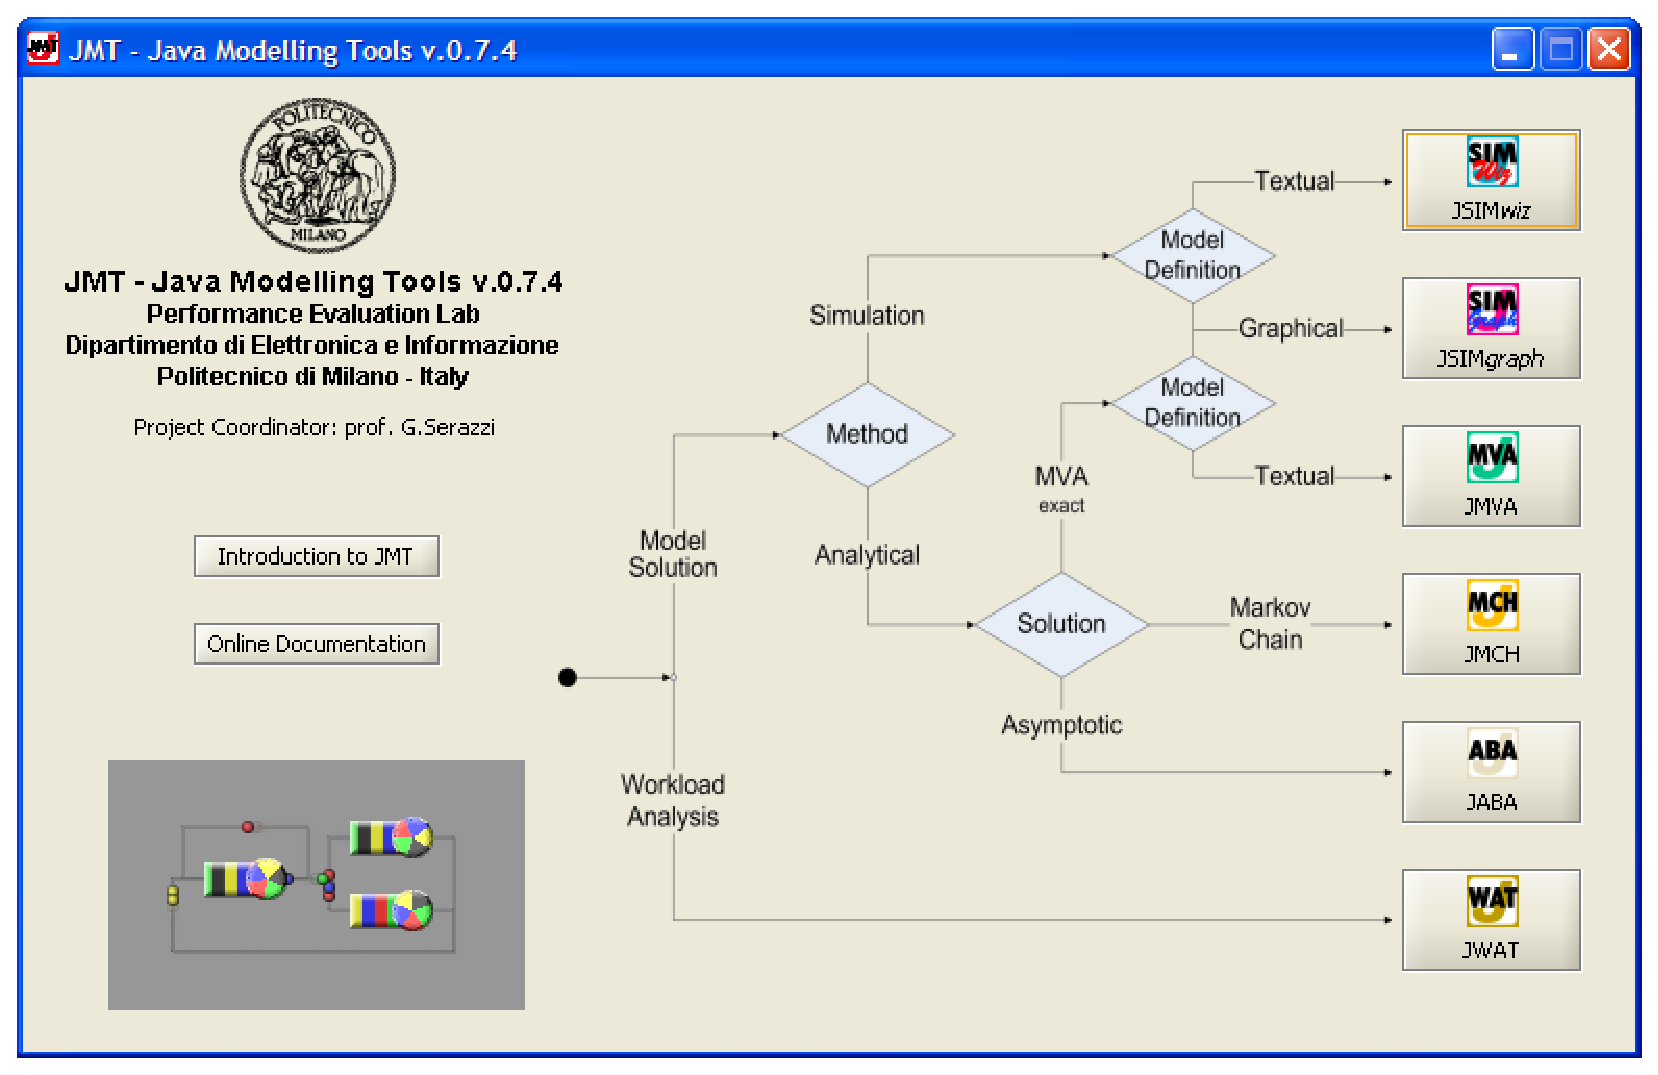
\includegraphics[scale=.5]{img/StartScreen}
    \end{center}
    \caption{The JMT suite Starting Screen}
    \label{fig:startscreen}
\end{figure}

This starting screen is used to select the application of the
suite to be executed by clicking on the corresponding button. The
flow chart should help the user to select the application that
best fits its needs.

In the following chapters the tools will be examined in details
and some examples are given. This manual is intended for the
general user that wants to learn how to interact with JMT.
Advanced users that want to learn details on internal data
structures, computational engines and XML interfaces should refer
to \emph{JMT system manual}.\\
Several other documents related to JMT description and
applications are provided with the suite. Click on \texttt{Online
Documentation} button to access the library. An exercise
book is also available.\\

%
% This document is free; you can redistribute it and/or modify
% it under the terms of the GNU General Public License as published by
% the Free Software Foundation; either version 2 of the License, or
% (at your option) any later version.
%
% This document is distributed in the hope that it will be useful, but
% WITHOUT ANY WARRANTY; without even the implied warranty of
% MERCHANTABILITY or FITNESS FOR A PARTICULAR PURPOSE.  See the GNU
% General Public License for more details.
%
% You should have received a copy of the GNU General Public License
% along with this document; if not, write to the Free Software
% Foundation, Inc., 51 Franklin Street, Fifth Floor, Boston, MA
% 02110-1301, USA.
%
% Author: Bertoli Marco
%
\chapter{JMVA}
\label{cha:jmva}
\section{Overview}
JMVA solves open, closed and mixed product form \cite{BCMP} queueing
networks with the exact MVA algorithm \cite{MVA}. In order to avoid
fluctuations of the solutions when the model contains load dependent
stations, the implemented algorithm is a stabilized version
\cite{AMVA} of the classic MVA algorithm.

Resources may be of two types: \emph{queueing} (either with
\texttt{load independent} or \texttt{load dependent} service times)
and \texttt{delay}. The model is described in alphanumeric way: user
is guided through the definition process by steps of a \emph{wizard}
interface (5 or 6 steps). What-if analyses, where a sequence of model are solved for different
values of parameters, are also possible (see \autoref{sec:jmva:whatif}). A graphical interface to describe the model in a user-friendly environment is also available, see \autoref{cha:jmodel} for details.

\subsection{Starting the alphanumeric MVA solver}
Selecting 
\includegraphics[scale=.5]{img/JMVAIcon} button on the
starting screen, \autoref{fig:jmva:Classes} window shows up.
\begin{figure}[htbp]
    \begin{center}
        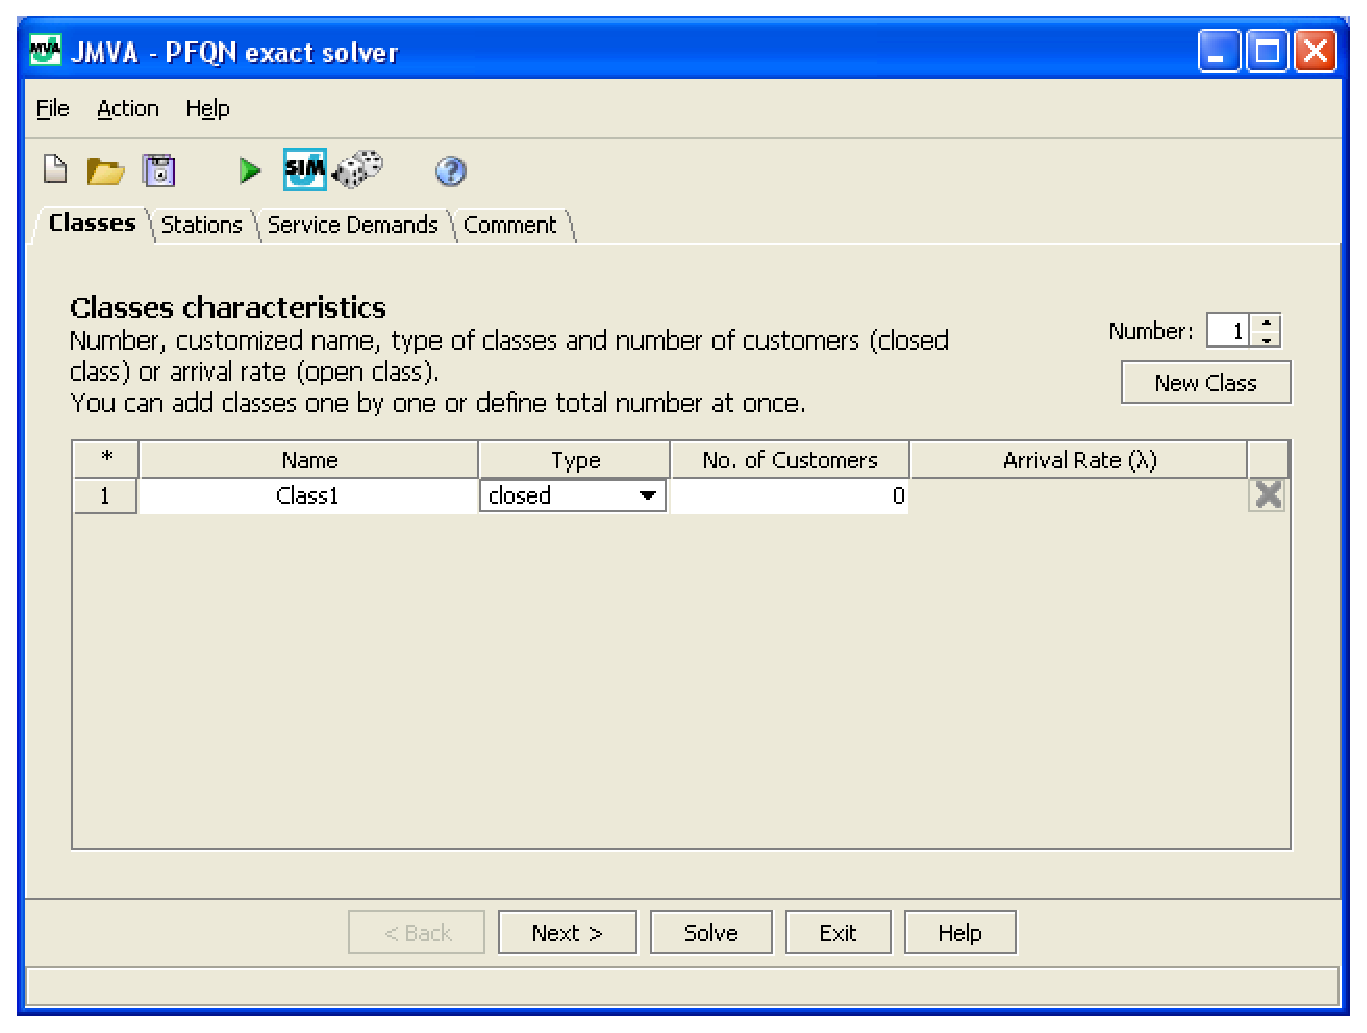
\includegraphics[scale=.5]{img/jmva/classes}
    \end{center}
    \caption{Classes tab}
    \label{fig:jmva:Classes}
\end{figure}
Three main areas are shown:
\begin{description}
\item[Menu :] it is organized into three groups of functions. To use a
menu, click on the menu heading and choose the appropriate option.
For the description of menu entries, see \autoref{sec:jmva:Menu}
\item[Toolbar :] contains some buttons to speed up access to JMVA functions
(e.g. New model, Open, Save\dots See \autoref{sec:jmva:Menu} for
details). If you move the mouse pointer over a button a tooltip will
be shown up.
\item[Page Area :] this is the core of the window. All MVA parameters are grouped in
different tabs. You can modify only a subset of them by selecting
the right tab, as will be shown later.
\end{description}

\section{Model definition}
Models with one or multiple customer classes provide estimates of
performance measures. For a brief description of basic terminology
please refer to \autoref{cha:glossary}.

In the case of single class models, the workload is characterized by
two inputs: the set of service demands, one for each resource, and
the workload intensity. On the other hand, in multiple class models,
a matrix of service demands is requested \cite{Lazowska}.

\subsection{Defining a new model}
To define a new model select toolbar button

\includegraphics[scale=.8]{img/jmva/new} or the \emph{New} command
from \emph{File} menu. The following parameters must be defined:
\begin{enumerate*}
\item \texttt{Classes} with their workload intensities (number of customer
$N$ for closed classes and arrival rate $\lambda$ for open classes)
\item \texttt{Stations} (service centers)
\item \texttt{Service demands} (or Service Times and Visits)
\item Optional short \texttt{Comment}
\end{enumerate*}

The execution of JMVA provides, for each class and each station, the
following performance indices:

\begin{itemize*}
\item Throughput
\item Queue Length
\item Residence Time
\item Utilization
\end{itemize*}

\noindent The following \emph{aggregate} indices are provided:
\begin{itemize*}
\item System Throughput
\item System Response Time
\item Average number of customers in the system
\end{itemize*}

\subsubsection{Input tabs}
As can be seen in \autoref{fig:jmva:Classes}, the parameters that
must be entered in order to define a new model are divided in four
tabs: \texttt{Classes}, \texttt{Stations}, \texttt{Service Demands}
and \texttt{Comment}.

Tabs number can become five, if you click  \emph{Service Times and
Visits} button in \texttt{Service Demands Tab}. As will be discussed
in \autoref{sec:jmva:ServiceDemand}, the \texttt{Service Demands
Tab} will be hidden and it will appear \texttt{Service Times Tab}
and \texttt{Visit Tab}. You can navigate through tabs:
\begin{itemize*}
\item using sequential wizard buttons, if enabled, at the bottom of
the window (\autoref{fig:jmva:Wizardbuttons})
\item using sequential buttons located in menu
\item using the tab selector, clicking on the corresponding
tab (\autoref{fig:jmva:Tabselector})
\end{itemize*}

\begin{figure}[htbp]
    \begin{center}
        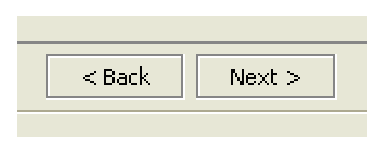
\includegraphics[scale=.5]{img/jmva/wizBut}
    \end{center}
    \caption{Wizard buttons}
    \label{fig:jmva:Wizardbuttons}
\end{figure}

\begin{figure}[htbp]
    \begin{center}
        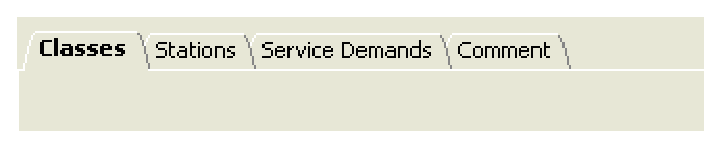
\includegraphics[scale=.5]{img/jmva/tabSel}
    \end{center}
    \caption{Tab selector}
    \label{fig:jmva:Tabselector}
\end{figure}

\subsection{Classes Tab}
An example screenshot of this tab can be seen in
\autoref{fig:jmva:Classes}. This tab allows to characterize customer
classes of the model. Your model will be a single class model if and
only if there will be only one class, closed or open. On the
contrary multiple class models will have at least two classes,
closed and/or open.

The number of classes in the model can be specified in the
corresponding input area, shown in \autoref{fig:jmva:ClassNum} and
can be modified using the keyboard or using the spin controls.

\begin{figure}[htbp]
    \begin{center}
        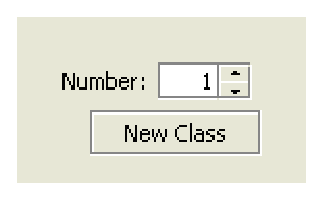
\includegraphics[scale=.5]{img/jmva/classNum}
    \end{center}
    \caption{Number of classes}
    \label{fig:jmva:ClassNum}
\end{figure}

Using the delete button
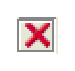
\includegraphics[scale=.6]{img/jmva/x} associated to a specific
class, a class can be removed provided that there will be at least
one class after the deletion. Similar result may be obtained using
spin controls, decreasing classes number; in this case last inserted
class will be removed.

Default class names are \emph{Class1}, \emph{Class2}, \dots
\emph{ClassN}. A model can be personalized by changing this names.

In \autoref{fig:jmva:3Classes} there are three classes of customers,
two closed and one open. The third class has the default name
\emph{Class3} while the other two classes have personalized names,
namely \emph{ClosedClass} and \emph{OpenClass}.

\begin{figure}[htbp]
    \begin{center}
        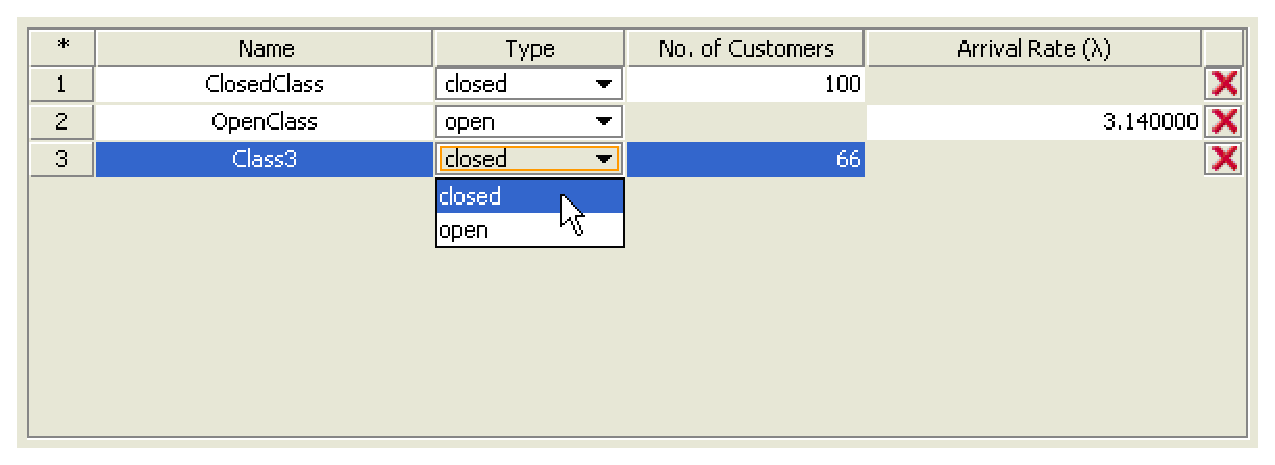
\includegraphics[scale=.5]{img/jmva/3classes}
    \end{center}
    \caption{Defining the classes types}
    \label{fig:jmva:3Classes}
\end{figure}

A class type can be \texttt{Open} or \texttt{Closed}. It is
important to define each class type because a closed class workload
is described by the number of customers in each class and the open
classes workload is described by the customer arrival rate for each
class.

As can be seen in \autoref{fig:jmva:3Classes}, a class type can be
selected in a combo-box. The input boxes \emph{No. of Customers
($N$)} referring to closed classes accept only positive integer
numbers; the input boxes of the \emph{Arrival Rate ($\lambda$)}
referring to open classes, accept positive real numbers
(\autoref{fig:jmva:workload}).

\begin{figure}[htbp]
    \begin{center}
        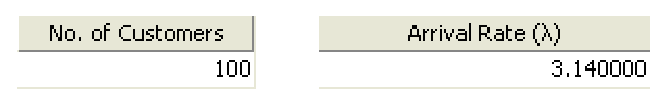
\includegraphics[scale=.5]{img/jmva/NL}
    \end{center}
    \caption{Workload definition of the number of customers of a closed
    class ($N=100$) and the arrival rate of an open class ($\lambda=3.14$)}
    \label{fig:jmva:workload}
\end{figure}

\subsection{Stations Tab}
The number of stations of the model can be specified in the
corresponding input area (\autoref{fig:jmva:stationNum}) and can be
modified using the keyboard or the spin controls.

\begin{figure}[htbp]
    \begin{center}
        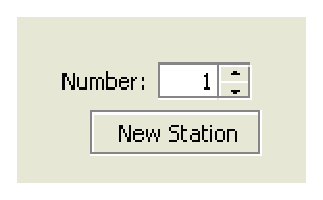
\includegraphics[scale=.5]{img/jmva/stationNum}
    \end{center}
    \caption{Number of stations}
    \label{fig:jmva:stationNum}
\end{figure}

Using the delete button
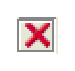
\includegraphics[scale=.6]{img/jmva/x} associated to a specific
station, a station can be removed provided that there will be at
least one station after the deletion. Similar result may be obtained
using spin controls, decreasing stations number; in this case last
inserted station will be removed.

Default station names are \emph{Station1}, \emph{Station2}, \dots
\emph{StationN}. In order to personalize your model, you can change
and give names other than default ones.

In \autoref{fig:jmva:stations} there is only one station with
default name \emph{Station4} and there are three stations with
personalized names: \emph{CPU}, \emph{Disk1} and \emph{Disk2}.

\begin{figure}[htbp]
    \begin{center}
        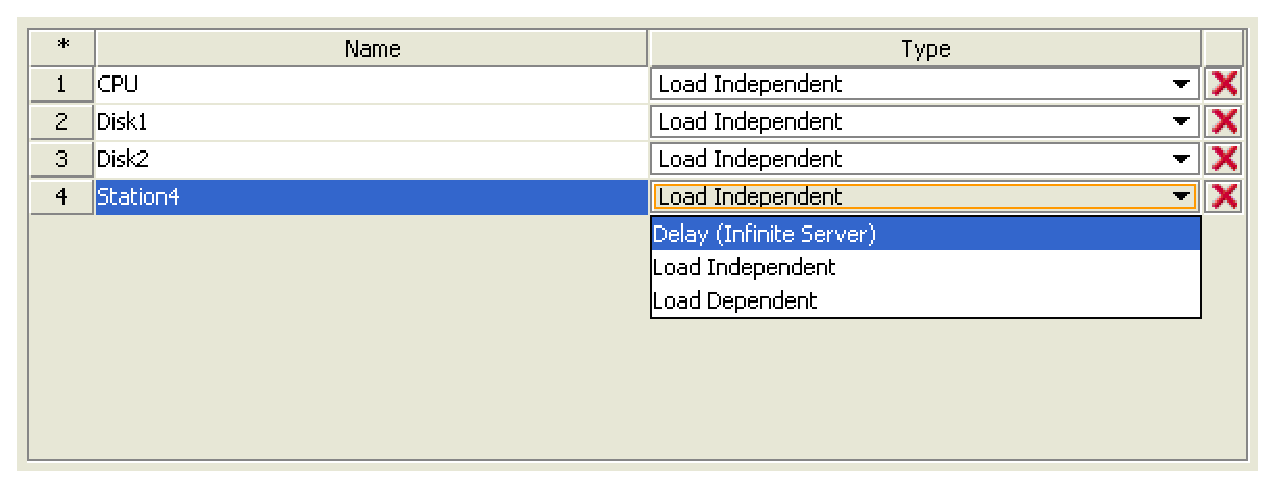
\includegraphics[scale=.5]{img/jmva/4stations}
    \end{center}
    \caption{Defining the stations type}
    \label{fig:jmva:stations}
\end{figure}

A station type can be \texttt{Load Independent}, \texttt{Load
Dependent} or \texttt{Delay}. You can insert in your model a
\texttt{Load Depend} center only if there is a unique closed
class\footnote{Multiclass, open and mixed models with load dependent
stations are not supported yet}; in all other cases the combo-box
will be disabled.

It is important to define each station type because if a station is
\texttt{Load Dependent} a set of service demand - or a set of
service times and the number of visit - must be defined (one service
demand/time for each possible value of queue length inside the
station).

In \autoref{sec:jmva:ServiceDemand} we will explain this concept
with more details.

\subsection{Service Demands, Service Times and Visits Tabs}
\label{sec:jmva:ServiceDemand} Service Demands can be defined in two
ways:
\begin{itemize*}
\item directly, by entering Service Demands ($D_{kc}$)
\item indirectly, by entering Service Times ($S_{kc}$) and Visits ($V_{kc}$)
\end{itemize*}

Service demand $D_{kc}$ is the total service requirement, that is
the average amount of time that a customer of class $c$ spends in
service at station $k$ during one interaction with the system, i.e.
it's complete execution. Service time $S_{kc}$ is the average time
spent by a customer of class $c$ at station $k$ for a single visit
at that station while $V_{kc}$ is the average number of visits at
that resource for each interaction with the system.

Remember that $D_{kc} = V_{kc} * S_{kc}$ so it's simple to compute
service demands matrix starting from service times and visits
matrixes. Inverse calculation is performed with the following
algorithm:
\[
V_{kj} = \left\{
\begin{array}{ccl} 1 & \textrm{if} & D_{kc} > 0 \\
0 & \textrm{if} & D_{kc} = 0 \end{array}\right.
\]
\[
S_{kc} = \left\{ \begin{array}{ccl} D_{kc} & \textrm{if} & D_{kc}
> 0 \\ 0 & \textrm{if} & D_{kc} = 0 \end{array}\right.
\]

\subsubsection{Service Demands Tab}
In this tab you can insert directly Service Demands $D_{kc}$ for
each pair \{station~$k$-class~$c$\} in the model. In
\autoref{fig:jmva:ServiceDemandsTab} a reference screenshot can be
seen: notice that a value for every $D_{kc}$ element of the
$D$-matrix has already been specified because default value assigned
to newly created stations is zero.

\begin{figure}[htbp]
    \begin{center}
        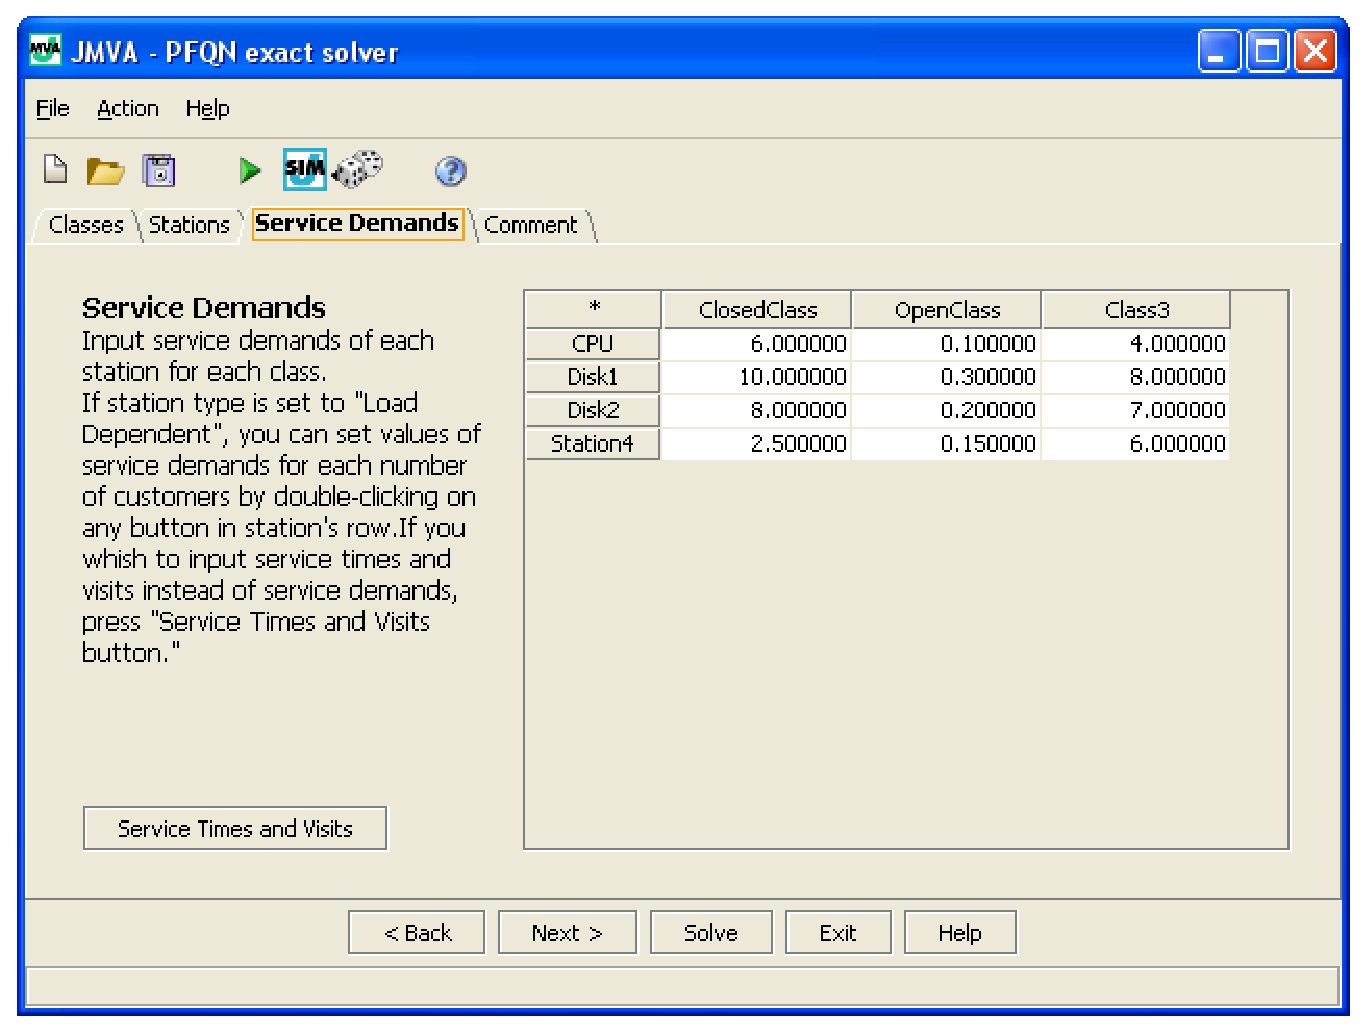
\includegraphics[scale=.5]{img/jmva/serviceDemands}
    \end{center}
    \caption{The Service Demands Tab}
    \label{fig:jmva:ServiceDemandsTab}
\end{figure}

In the example of \autoref{fig:jmva:ServiceDemandsTab}, each job of
type \emph{ClosedClass} requires an average service demand time of 6
sec to \emph{CPU}, 10 sec to \emph{Disk1}, 8 sec to
\emph{Disk2} and 2.5 sec to \emph{Station4}.\\
On the other hand, a job of type \emph{OpenClass} requires on
average 0.1 sec of \emph{CPU} time, 0.3 sec of \emph{Disk1} time,
0.2 sec of \emph{Disk2} time and 0.15 sec of \emph{Station4} time to
be processed by the system.

If the model contains any load dependent station, the behavior of
\autoref{fig:jmva:LD} will be shown.

\begin{figure}[htbp]
    \begin{center}
        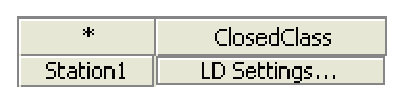
\includegraphics[scale=.5]{img/jmva/ld}
    \end{center}
    \caption{Defining a \emph{load dependent} station service demand}
    \label{fig:jmva:LD}
\end{figure}

By double-clicking on \emph{LD Settings\dots} button a window will
show up and that can be used to insert the values of the service
demands for each possible number of customer inside the station.
That values can be computed by evaluating an analytic function as
shown in \autoref{fig:jmva:LDEdit}. The list of supported operators
and more details are reported in \autoref{sec:jmva:JEP}.

\begin{figure}[htbp]
    \begin{center}
        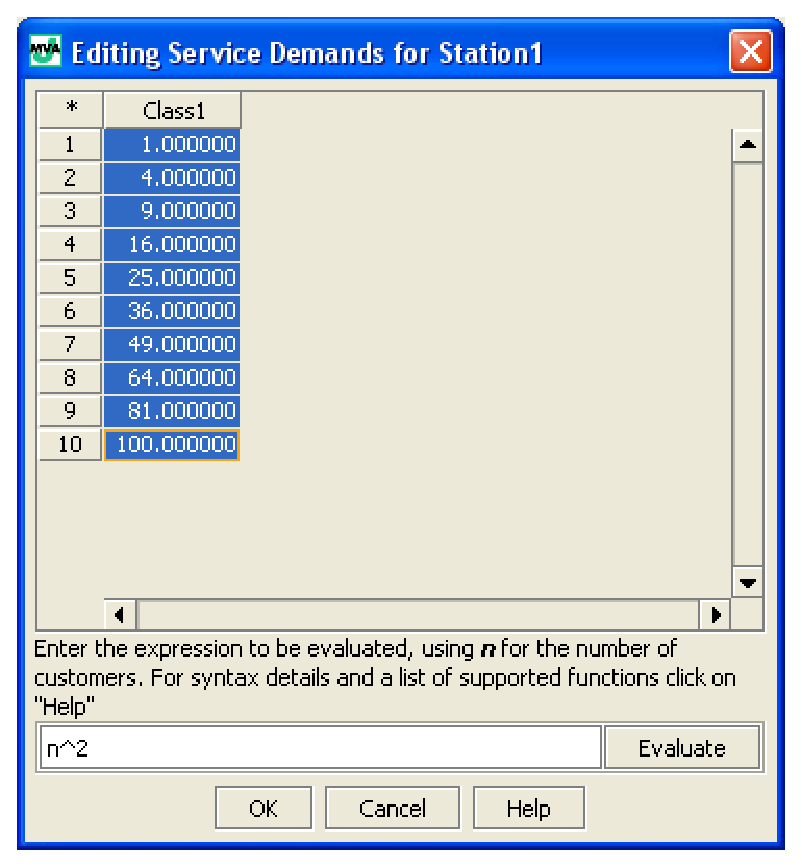
\includegraphics[scale=.5]{img/jmva/ldEdit}
    \end{center}
    \caption{Load Dependent editing window}
    \label{fig:jmva:LDEdit}
\end{figure}

\subsubsection{Service Times and Visits Tabs}
In the former tab you can insert the Service Times $S_{kc}$ for each
pair \{station~$k$-class~$c$\} in the model, in the latter you can
enter the visits number $V_{kc}$ (See \autoref{fig:jmva:visits}).

\begin{figure}[htbp]
    \begin{center}
        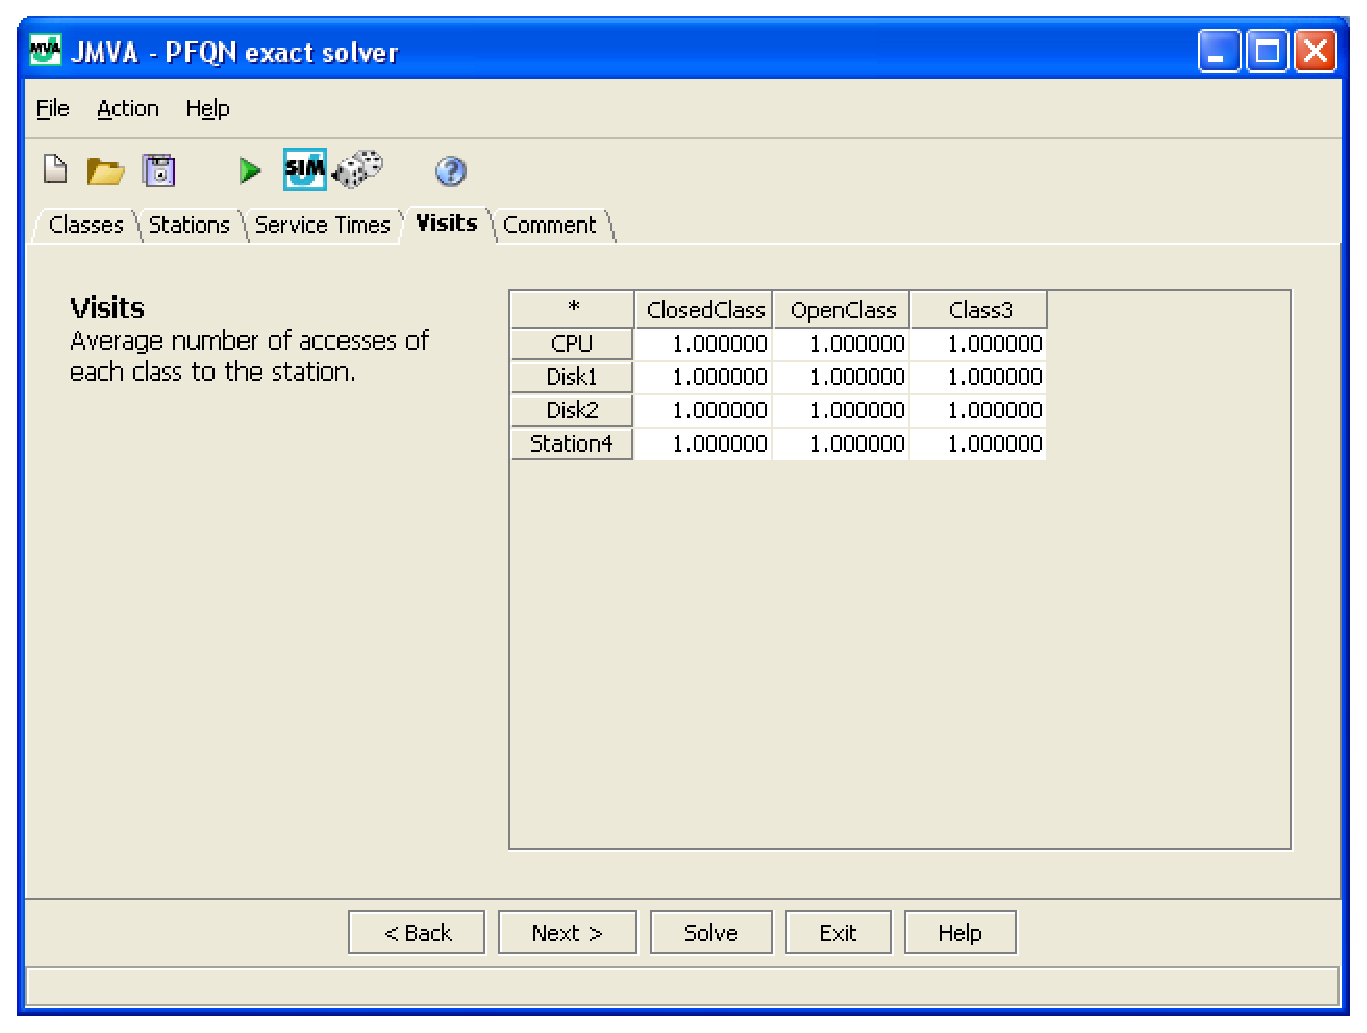
\includegraphics[scale=.5]{img/jmva/visits}
    \end{center}
    \caption{Visits Tab}
    \label{fig:jmva:visits}
\end{figure}

The layout of these tabs is similar to the one of the
\texttt{Service Demand Tab} described in the previous paragraph. The
default value for each element of the Service Times ($S$) matrix is
zero, while it's one for Visits' matrix elements.

In current model contains load dependent stations, the behavior of
\texttt{Service Times Tab} for their parametrization will be
identical to the one described on the previous paragraph for
\texttt{Service Demands Tab}. On the other hand \texttt{Visits Tab}
behavior won't change as load dependency is a property of service
times and not of visits.

\subsection{What-if Tab}
\label{sec:jmva:whatif} This Tab is used to perform a what-if
analysis, i.e. solve multiple models changing the value of a
\texttt{control parameter}. In \autoref{fig:jmva:whatifDisabled} is
shown this panel when what-if analysis is disabled.

\begin{figure}[htbp]
    \begin{center}
        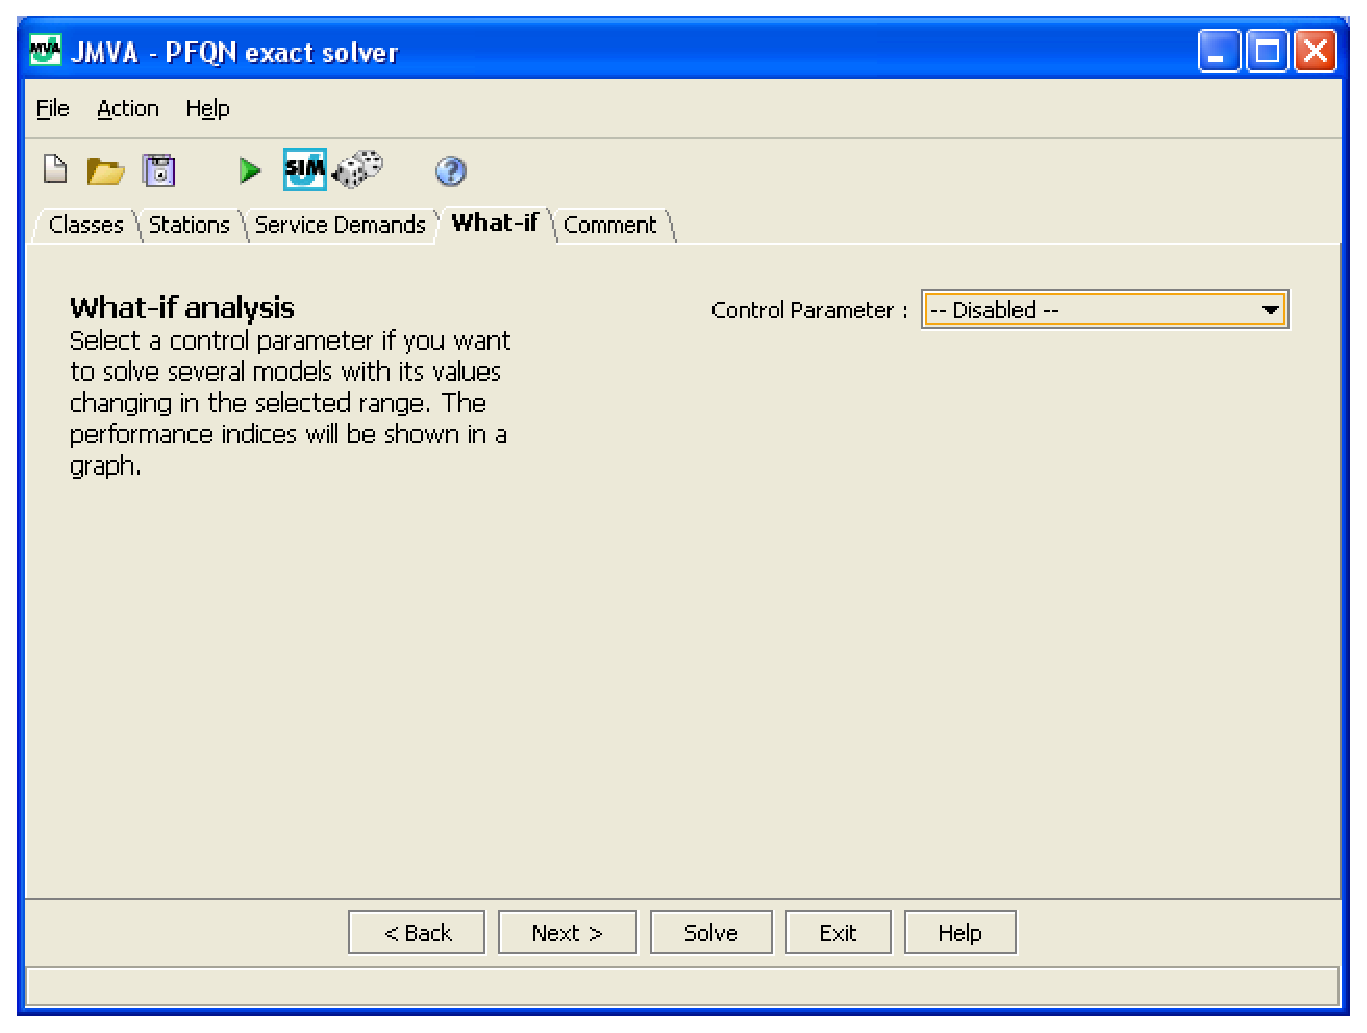
\includegraphics[scale=.5]{img/jmva/whatifDisabled}
    \end{center}
    \caption{What-if Tab - Disabled analysis}
    \label{fig:jmva:whatifDisabled}
\end{figure}

The first parameter to be set is the \texttt{control parameter} i.e.
the parameter that will be changed to solve different models in a
selected range. Five choices are possible:
\begin{description*}
\item[Disabled :] disables what-if analysis, so only a single queueing network
model, specified in the previous steps, will be solved. This is the
\emph{default} option.
\item[Customer Numbers :] different models will be
executed by changing the \texttt{number of customers} of a single
\texttt{closed} class or of every closed class proportionally. This
option is available only when current model has at least one closed
class.
\item[Arrival Rates :] different models will be
executed by changing \texttt{arrival rate} of a single \texttt{open}
class or of every open class proportionally. This option is
available only when current model has at least one open class.
\item[Population Mix :] the total number of customers will be kept
constant, but the population mix (i.e. the ratio between
\texttt{number of customers} of selected closed class $i$ and the
total number of customers in the system $\beta_i = N_i / \sum_k
N_k$). This option is available only when current model has two
closed classes.
\item[Service Demands :] different models will be solved changing
the \texttt{service demand} value of a given station for a given
class or for all classes proportionally. This option is available
only for \texttt{load independent} and \texttt{delay} stations.
\end{description*}

Whenever a control parameter is selected, the window layout will be
changed to allow the selection of a valid range of values for it.
For example in \autoref{fig:jmva:whatifDemands} \texttt{Service
Demands} control parameter was selected. On the bottom of the
window, a riepilogative table is presented: depending on selected
control parameter, that table is used to show the \emph{initial
state} of involved parameters. Every class currently selected for
what-if analysis is shown in red.

\begin{figure}[htbp]
    \begin{center}
        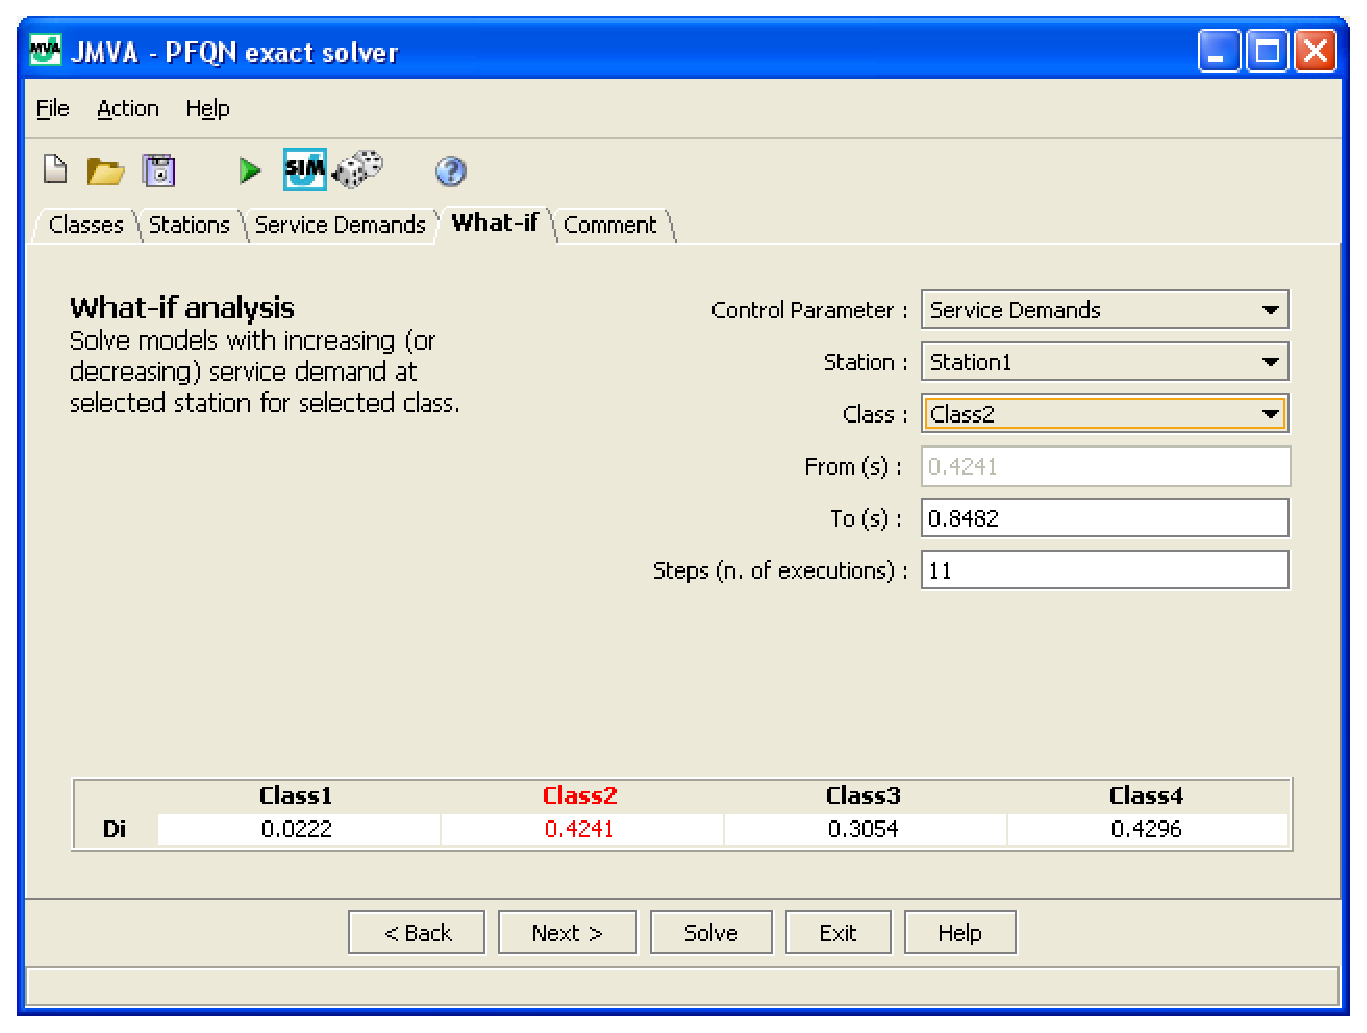
\includegraphics[scale=.5]{img/jmva/whatifDemands}
    \end{center}
    \caption{What-if Tab - Service Demands}
    \label{fig:jmva:whatifDemands}
\end{figure}

A brief description of each field is now presented:
\begin{description*}
\item[Station :] available only with \texttt{Service Demands} control
parameter. This combo box allows to select at which station service
demand values will be modified.
\item[Class :] allow to select for which class the selected
parameter will be changed. A special value, namely \texttt{All
classes proportionally}, is used to modify the control parameter for
each class keeping constant the proportion between different
classes\footnote{for example, in a model with two closed classes
with population vector (2,6), the following models can be executed:
(1,3), (2,6), (3,9), (4, 12), \dots}. This special value is not
available in \texttt{Population Mix} analysis as we are changing the
proportion of jobs between two closed classes.
\item[From :] the initial value of what-if analysis. It was chosen
to leave this value fixed to the initial value specified by the user
in the previous steps to avoid confusions, so this field acts as a
reminder. The only exception is when \texttt{Population Mix} is
changed, in that case it's allowed to modify this value too.
\item[To :] the final value of what-if analysis. Please notice that
this value can be greater or smaller than \texttt{From} value and is
expressed in the same measure unit. Whenever \texttt{All classes
proportionally} option is selected, both \texttt{From} and
\texttt{To} values are expressed as percentages of initial values
(specified in the previous steps and reminded in the table at the
bottom of the panel, see \autoref{fig:jmva:whatifDemands}), in the
other situations they are considered as absolute values for the
chosen parameter.
\item[Steps :] this is chosen number of executions i.e. the number
of different models that will be solved. When control parameter is
\texttt{Customer Numbers} or \texttt{Population Mix}, the model can
be correctly specified only for integer values of population. JMVA
will perform a fast computation to find the maximum allowed number
of executions given current \texttt{From} and \texttt{To} values: if
user specify a value bigger than that, JMVA will use the computed
value.
\end{description*}


\subsection{Comment Tab}
In this Tab, a short - optional - comment about the model can be
inserted; it will be saved with the other model parameters.

\subsection{Expression Evaluator}
\label{sec:jmva:JEP} An expression evaluator is used for the
definition of service demands or service times of a load dependent
station. It allows to specify times as an analytic function of $n$
where $n$ is the number of customer inside the station.

Expression are evaluated using
\emph{JEPLite}\footnote{http://jeplite.sourceforge.net/} (Java Math
Expression Parser enlited) package which supports all operators
enumerated in \autoref{tab:jmva:Operators} and all functions
enumerated in \autoref{tab:jmva:Functions}.

\begin{table}[htbp]
\begin{center}
\begin{tabular}{|c|c|}
Operator & Symbol\\
\hline
Power & $^{\wedge}$\\
Unary Plus, Unary Minus & $+n$, $-n$\\
Modulus & $\%$\\
Division & $/$ \\
Multiplication & $*$\\
Addition, Subtraction & $+$, $-$\\
\hline
\end{tabular}
\end{center}
\caption{List of all supported operators ordered by priority}
\label{tab:jmva:Operators}
\end{table}

\begin{table}[htbp]
\begin{center}
\begin{tabular}{|c|c|}
Function & Symbol\\
\hline
Sine & sin()\\
Cosine & cos()\\
Tangent & tan()\\
Arc Sine & asin()\\
Arc Cosine & acos()\\
Arc Tangent & atan()\\
Hyperbolic Sine & sinh()\\
Hyperbolic Cosine & cosh()\\
Hyperbolic Tangent & tanh()\\
Inverse Hyperbolic Sine & asinh()\\
Inverse Hyperbolic Cosine & acosh()\\
Inverse Hyperbolic Tangent & atanh()\\
Natural Logarithm & ln()\\
Logarithm base 10 & log()\\
Absolute Value / Magnitude & abs()\\
Random number $[0,1]$ & rand()\\
Square Root & sqrt()\\
Sum & sum()\\
\hline
\end{tabular}
\end{center}
\caption{List of supported functions for the load dependent service
times} \label{tab:jmva:Functions}
\end{table}

\subsection{Model Solution}
\label{sec:jmva:solution}Use \texttt{Solve} command to solve the
model. If the model specify a what-if analysis, please refer to
\autoref{sec:jmva:solutionWhatif}. Model results will be shown on a
separate window, like the one of \autoref{fig:jmva:results}.

\begin{figure}[htbp]
    \begin{center}
        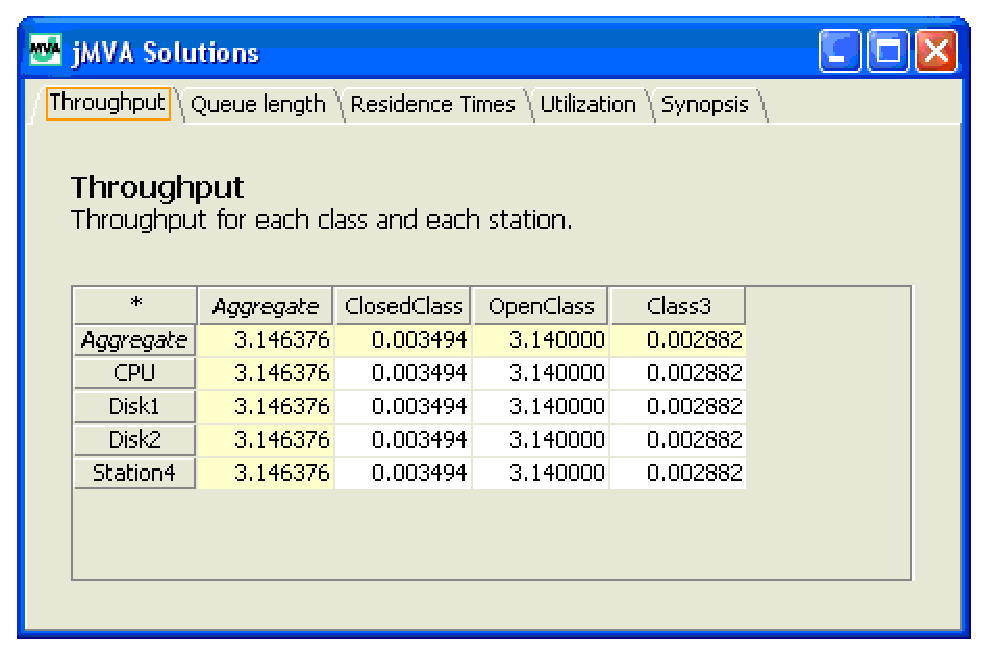
\includegraphics[scale=.5]{img/jmva/results}
    \end{center}
    \caption{Model Solution (Throughput Tab)}
    \label{fig:jmva:results}
\end{figure}

Using the tab selector, all the other computed performance indices
can be seen: Throughput, Queue lengths, Residence Times,
Utilizations and a synopsis panel with schematic report of input
model. Both results and synopsis tab data can be copied to clipboard
with \texttt{CTRL+C} keyboard shortcut.

When open classes are used, the resource saturation control is
performed. For multiple class models, the following inequality must
be satisfied:
\[
{\max_k {\sum_c{\lambda_c * D_{kc}}}} < 1
\]
This inequality ensures that no service center is saturated as a
result of the combined loads of all the classes. Let us consider, as
example, the model with the classes shown in
\autoref{fig:jmva:3Classes} with the D-matrix shown in
\autoref{fig:jmva:ServiceDemandsTab} Since $\lambda = 3.14 < 3.33 =
1 / 0.3 = 1 / D_{max}$ the model is not in saturation and the
\texttt{Solve} command will be executed correctly.

In this example, substituting $D_{\textrm{Disk1-OpenClass}}$ with
values $\geq 1/3.14 \approx 0.318$ will cause the saturation of
resource \emph{Disk1} and the error message of
\autoref{fig:jmva:saturation} will appear.

\begin{figure}[htbp]
    \begin{center}
        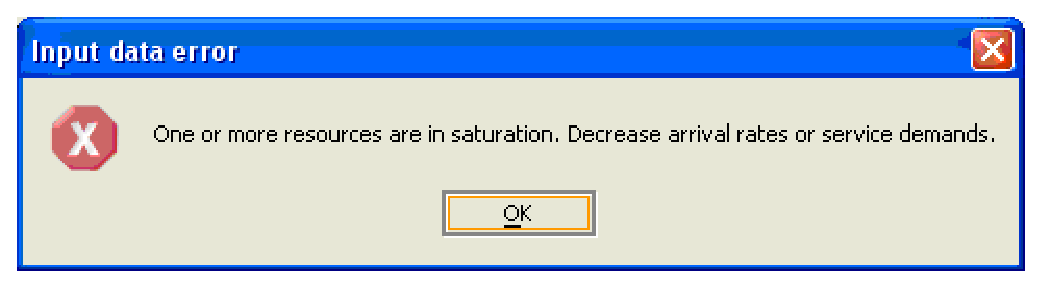
\includegraphics[scale=.5]{img/jmva/saturation}
    \end{center}
    \caption{Input data error message }
    \label{fig:jmva:saturation}
\end{figure}

\subsection{Model Solution - What-if analysis}
\label{sec:jmva:solutionWhatif}Use \texttt{Solve} command to solve
the model. During model solution, a progress window, see
\autoref{fig:jmva:progress}, shows up. It displays the cumulative
number of models currently solved, the total number of models to be
solved and the elapsed time.

\begin{figure}[htbp]
    \begin{center}
        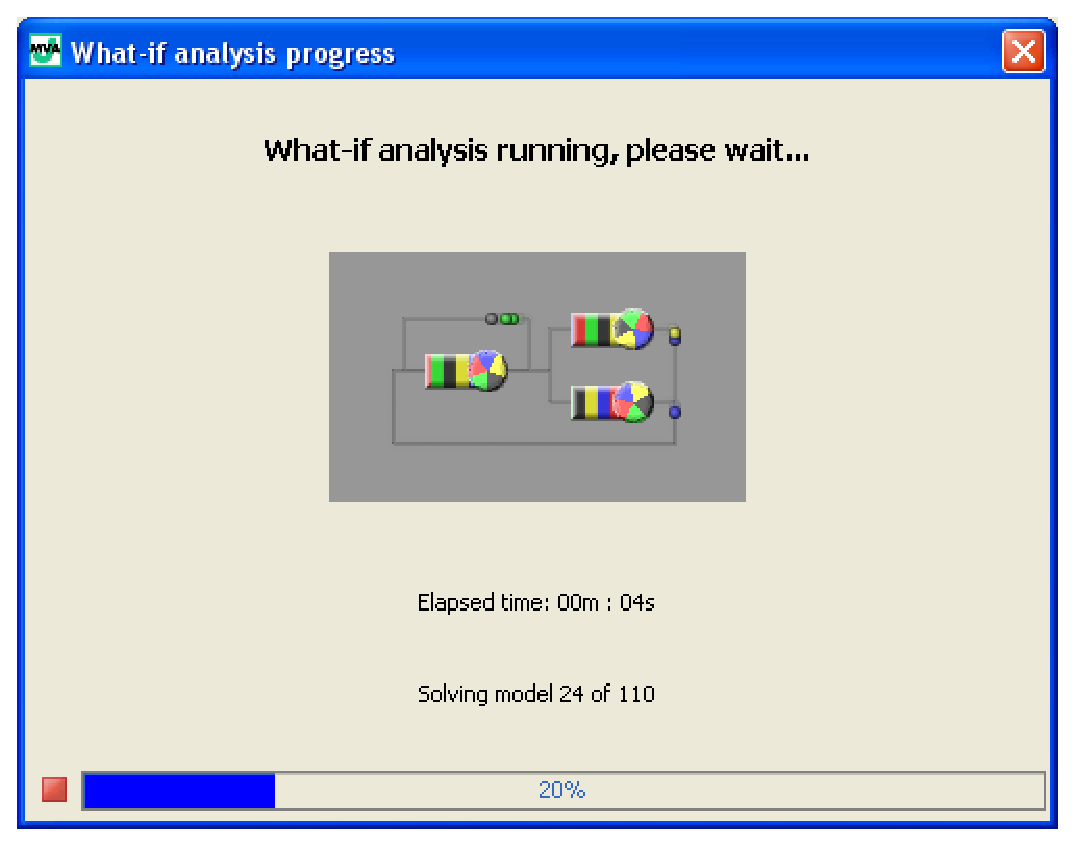
\includegraphics[scale=.5]{img/jmva/progress}
    \end{center}
    \caption{Model Solution progress window}
    \label{fig:jmva:progress}
\end{figure}

At the end of the solution, results will be shown in a separate
window, see \autoref{fig:jmva:graphical}.
\begin{figure}[htbp]
    \begin{center}
        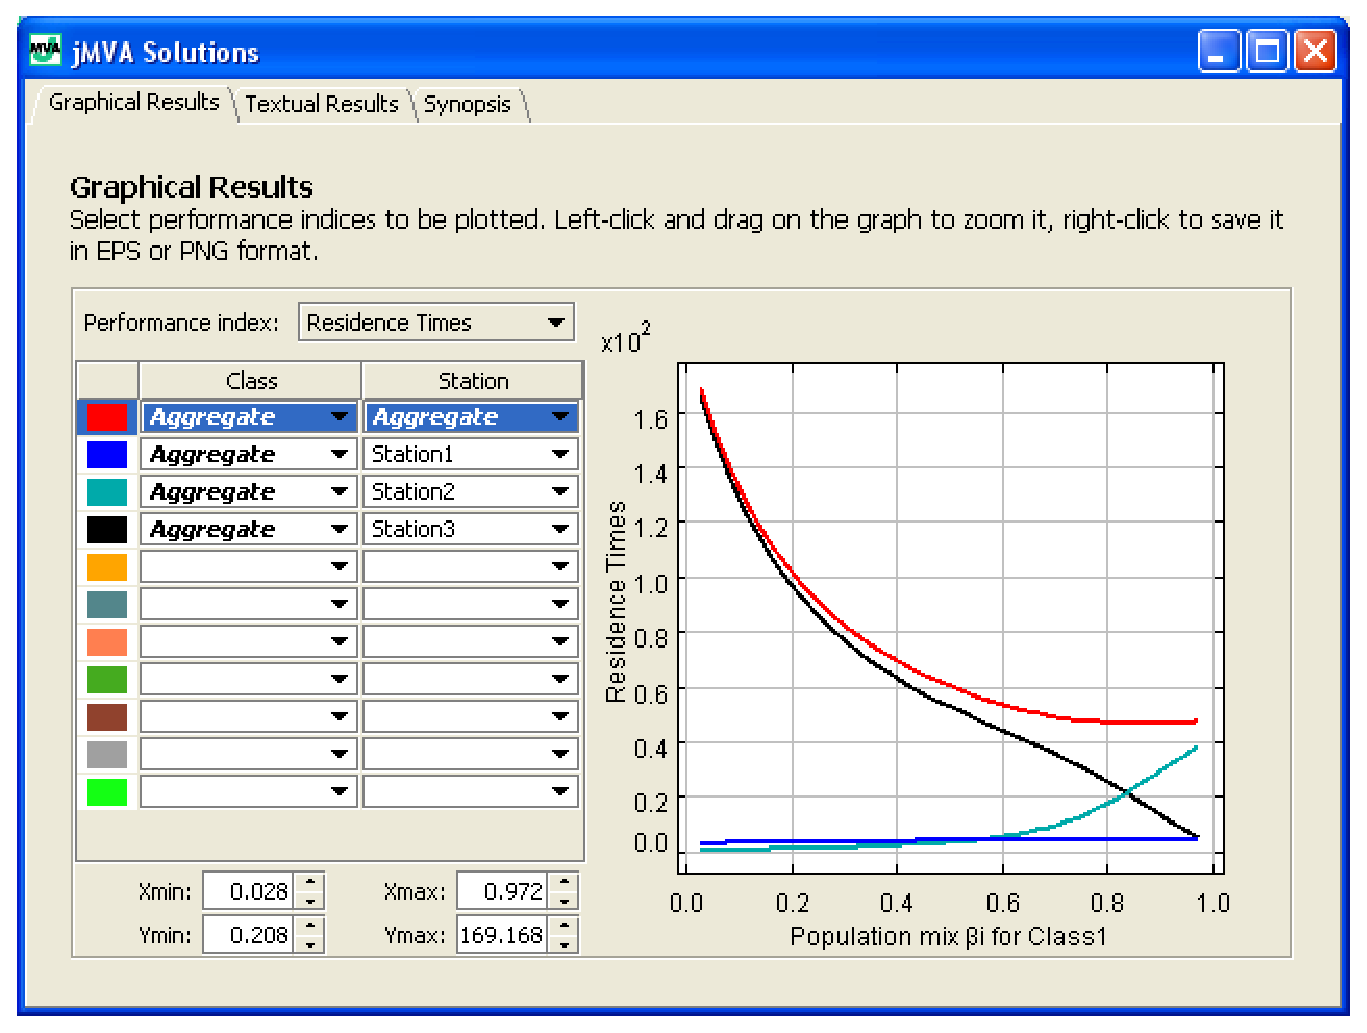
\includegraphics[scale=.5]{img/jmva/Graphical}
    \end{center}
    \caption{Model Solution - Graphical Results Tab}
    \label{fig:jmva:graphical}
\end{figure}
This tab allows to show in a plot the relation between the chosen
control parameter (see \autoref{sec:jmva:whatif}) and the
performance indices computed by the analytic engine.

The combo box \texttt{Performance Index} allows to select the
performance index to be plotted in the graph, while in the table
below, users can select the resource and the class considered.
\begin{itemize*}
\item The first column is fixed and lists all available colors to be
used in the graph.
\item The second column, named \texttt{Class}, is used to select the
class considered in the graph. The special value \texttt{Aggregate}
is used for the aggregate measure for all classes. If input model is
single-class, the class is selected by default for each row.
\item The final column, named \texttt{Station}, is used to select the
station considered in the graph. The special value
\texttt{Aggregate} is used for the aggregate measure for the entire
network. Note that the \texttt{Aggregate} value is not valid when
the \texttt{Utilization} performance index is selected.
\end{itemize*}

In addition to the \emph{center} performance indices (i.e.
\texttt{Throughput}, \texttt{Queue length}, \texttt{Residence
Times}, \texttt{Utilization}), three \emph{system} performance
indices are provided  in the \texttt{Performance Index} combo box
(\texttt{System Response Time}, \texttt{System Throughput},
\texttt{Number of Customers}). This \emph{system} indices can be
easily obtained by selecting the special \texttt{Aggregate} value
for both \texttt{Class} and \texttt{Station} columns of the
corresponding center indices (see \autoref{cha:glossary} for the
definition of the performance indices), but they were provided here
as a \emph{shortcut}. As we are referring to aggregate measures, the
selection of reference class and station is not significant and, in
this case, the table in the left of \autoref{fig:jmva:graphical}
will not be shown.

On the bottom-left corner of the window, users can modify minimum
and maximum value of both X and Y axis of the plot. JMVA is designed
to automatically best-fit the plot in the window but this controls
allow the user to specify a custom range or zoom on the plot.
Another fast method to perform a zoom operation is to left-click and
drag a rectangle on the graphic window (see
\autoref{fig:jmva:zoomDrag}) or right-click on it and select
\texttt{Zoom in} or \texttt{Zoom out} options. To automatically
reset the best-fit scale users can right-click on the graphic window
and select \texttt{Original view} option.

\begin{figure}[htbp]
    \begin{center}
        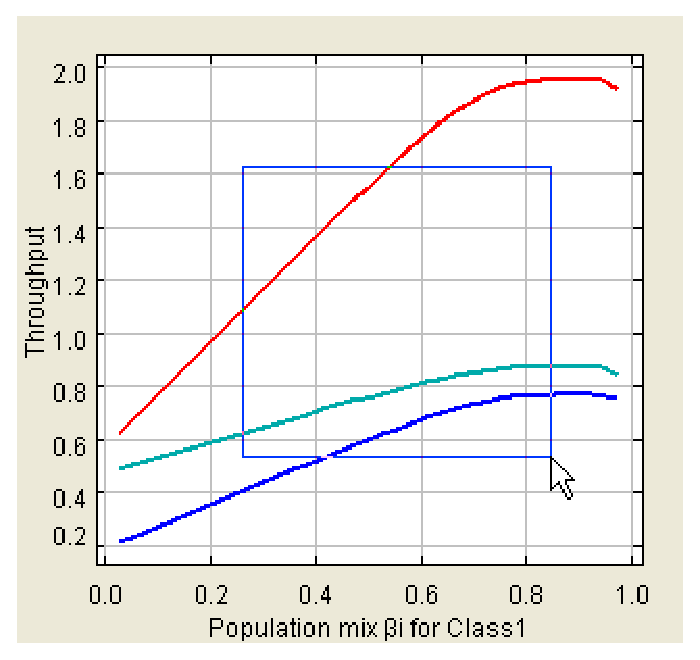
\includegraphics[scale=.5]{img/jmva/whatIfDrag}
    \end{center}
    \caption{Zoom operation on the plot}
    \label{fig:jmva:zoomDrag}
\end{figure}

The graphic window allows to export plots as image to be included in
documents and presentations. To save current graph as image,
right-click on the graphic and select \texttt{Save as\dots} option.
A dialog will be shown to request the name of the file and the
format. Currently supported format are Portable Network Graphics -
PNG - (raster) and Encapsulated PostScript - EPS - (vectorial,
currently only black and white).

The second tab of the solution window, shown in
\autoref{fig:jmva:textualResults}, is used to display the solutions
of each execution of the analytic algorithm.

\begin{figure}[htbp]
    \begin{center}
        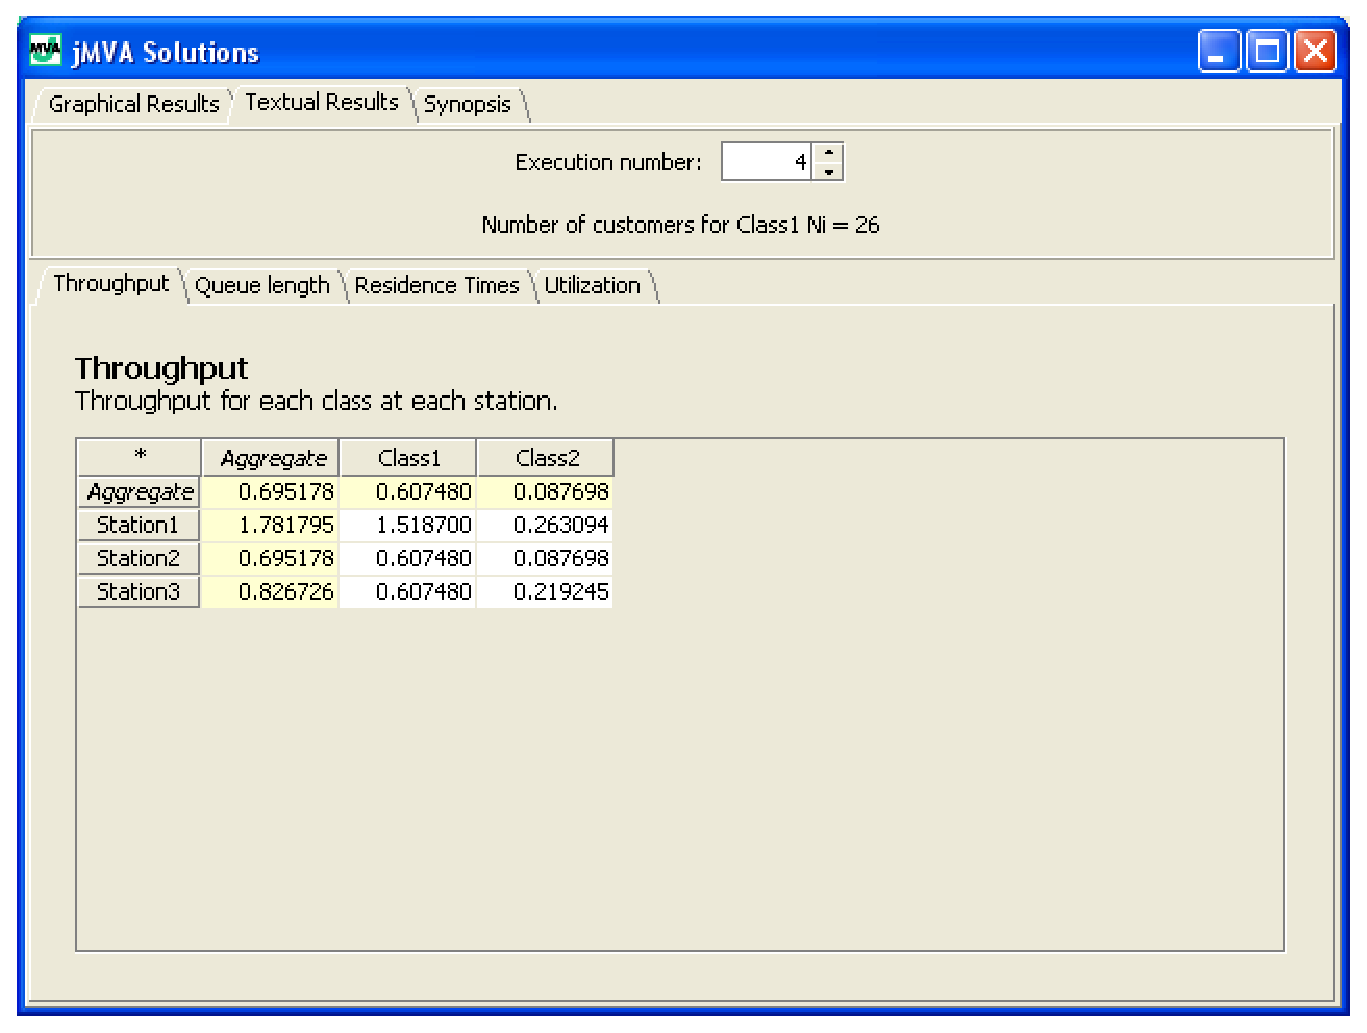
\includegraphics[scale=.5]{img/jmva/textualResults}
    \end{center}
    \caption{Model Solution - Textual Results Tab}
    \label{fig:jmva:textualResults}
\end{figure}

This Tab has the same structure of the results window without
What-if analysis (described in \autoref{sec:jmva:solution}) but
allows to select the execution to be shown in the field
\texttt{Execution Number}. By entering requested execution number in
the spinner, or using the \emph{up} and \emph{down} arrows, user can
cycle between all the computed performance indices for each
execution. Just below the spinner, a label gives information on the
value of the control parameter for the currently selected execution.

\subsection{Modification of a model}
To modify system parameters return to the main window and enter new
data. After the modifications, if you use \texttt{Solve} command, a
new window with model result will show. You can \texttt{save} this
new model with the previous name - overwriting the previous one - or
\texttt{save} it with a different name or in a different directory.

\section{Menu entries}
\label{sec:jmva:Menu}
\subsection{File}
\subsubsection{New}
Use this command in order to create a new JMVA model.

\noindent
\begin{tabular}{ll}
Shortcut on Toolbar: & 
\includegraphics[scale=.8]{img/jmva/new}\\
Accelerator Key: & CTRL+N
\end{tabular}

\subsubsection{Open}
Use this command to open an existing model. You can only open one
model at time, to edit two or more models start more than one
instance of JMVA. If current model was modified since its creation
or last save action, a popup window will be shown for confirmation.

It's possible to open not only models saved with JMVA (*.jmva), but
also with other programs of the suite (for example JABA *.jaba, JSIM
*.jsim and JMODEL *.jmodel). Whenever a foreign data file is opened, a
conversion is performed and error/warnings occurred during
conversion will be reported in a window.

Models are stored in XML format, see \emph{JMT system manual} for a
detailed description.

\noindent
\begin{tabular}{ll}
Shortcut on Toolbar: & 
\includegraphics[scale=.8]{img/jmva/open}\\
Accelerator Key: & CTRL+O
\end{tabular}

\subsubsection{Save}
Use this command in order to save the active document with its
current name in the selected directory.

When you save a document for the first time, JMVA displays the Save
As dialog box so you can rename your document. If you save a model
after its resolution, results are stored with model definition data.

\noindent
\begin{tabular}{ll}
Shortcut on Toolbar: & 
\includegraphics[scale=.8]{img/jmva/save}\\
Accelerator Key: & CTRL+S
\end{tabular}

\subsubsection{Exit}
Use this command in order to end a JMVA session. You can also use
the Close command on the application Control menu. If current model
was modified since its creation or last save action, a popup window
will be shown for confirmation.

\noindent
\begin{tabular}{ll}
\\
Accelerator Key: & CTRL+Q
\end{tabular}

\subsection{Action}
\subsubsection{Solve}
Use this command when model description is terminated and you want
to start the solution of the model. At the end of the process the
window in \autoref{fig:jmva:results} will popup.

\noindent
\begin{tabular}{ll}
Shortcut on Toolbar: & 
\includegraphics[scale=.8]{img/jmva/solve}\\
Accelerator Key: & CTRL+L
\end{tabular}

\subsubsection{Randomize}
Use this command in order to insert random values into Service
Demands - or Service Times - table. Generated values are
automatically adjusted to avoid saturation of resources.

\noindent
\begin{tabular}{ll}
Shortcut on Toolbar: & 
\includegraphics[scale=.8]{img/jmva/randomize}\\
Accelerator Key: & CTRL+R
\end{tabular}

\subsubsection{Import in JSIM}
This command will import current model into JSIM to solve it using
simulator. A simple parallel topology is derived from number of
visits at each station and generated model is equivalent to original
one.

\noindent
\begin{tabular}{ll}
Shortcut on Toolbar: & 
\includegraphics[scale=.8]{img/jmva/toJSIM}\\
Accelerator Key: & CTRL+G
\end{tabular}

\subsection{Help}
\subsubsection{JMVA Help}
Use this command to display application help. From the initial
window, you can jump to step-by-step instructions that show how use
JMVA and consult various types of reference information.

Once you open Help, you can click the Content button whenever you
want to return to initial help window.

\noindent
\begin{tabular}{ll}
Shortcut on Toolbar: & 
\includegraphics[scale=.8]{img/jmva/help}\\
Accelerator Key: & CTRL+Q
\end{tabular}

\subsubsection{About}
Use it in order to display information about JMVA version and
credits.

\section{Examples}
In this section we will describe some examples of model
parametrization and solution using MVA exact solver. Step-by-step
instructions are provided in five examples:
\begin{enumerate*}
\item A single class closed model with three load independent stations and a delay service
center (\autoref{sec:jmva:example1})
\item A multiclass open model with two classes and three load independent
stations (\autoref{sec:jmva:example2})
\item A single class closed model with a load dependent station and
a delay (\autoref{sec:jmva:example3})
\item A multiclass mixed model with three stations (\autoref{sec:jmva:example4})
\item A multiclass closed model where a what-if analysis is used to find optimal
Population Mix values (\autoref{sec:jmva:example5})
\end{enumerate*}


\subsection{Example 1 - A model with a single closed class}
\label{sec:jmva:example1} Solve the single class model specified in
\autoref{fig:jmva:Example1topology}.
\begin{figure}[htbp]
    \begin{center}
        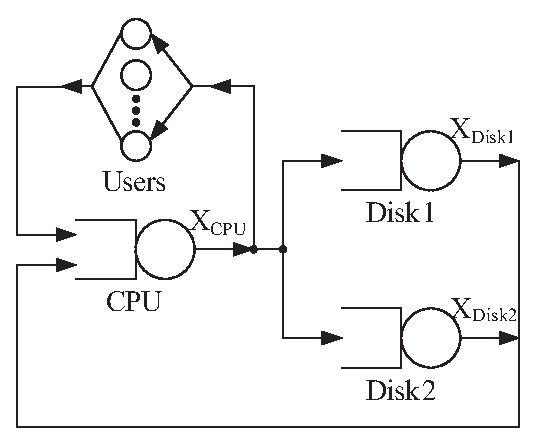
\includegraphics[scale=.65]{img/jmva/example1}
    \end{center}
    \caption{Example 1 - network topology}
    \label{fig:jmva:Example1topology}
\end{figure}
The customer class, named \emph{ClosedClass} has a population of $N
= 3$ customers.

There are four stations, three are of load independent type (named
\emph{CPU}, \emph{Disk1} and \emph{Disk2}) and one is of delay type
(named \emph{Users}). \emph{Users} delay station represents user's
\emph{think time} ($Z = 16$ s) between interaction with the system.
Service times and visits for stations are reported in
\autoref{tab:jmva:example1ServTimes}.

\begin{table}[htbp]
\begin{center}
\begin{tabular}{c|r|r|r|r|}
& \multicolumn{1}{c|}{CPU} & \multicolumn{1}{c|}{Disk1} & \multicolumn{1}{c|}{Disk2} & \multicolumn{1}{c|}{Users}\\
\hline
Service Times [s] & $0.006$ & $0.038$ & $0.030$ & $16.000$\\
Visits & $101.000$ & $60.000$ & $40.000$ & $1.000$\\
\hline
\end{tabular}
\end{center}
\caption{Example 1 - service times and visits}
\label{tab:jmva:example1ServTimes}
\end{table}

\subsubsection{Step 1 - Classes Tab}
\begin{itemize*}
\item use New command to create a new jMVA document
\item by default, you have already a \texttt{Closed} class
\item if you like, substitute default \emph{Class1} name with a customized
one (\emph{ClosedClass} in our example)
\item complete the table with workload intensity (number of customers). Remember that
intensity of a closed class N must be a positive integer number; in
this case, 3
\end{itemize*}

At the end of this step, the \texttt{Classes Tab} should look like
\autoref{fig:jmva:example1Classes}.

\begin{figure}[htbp]
    \begin{center}
        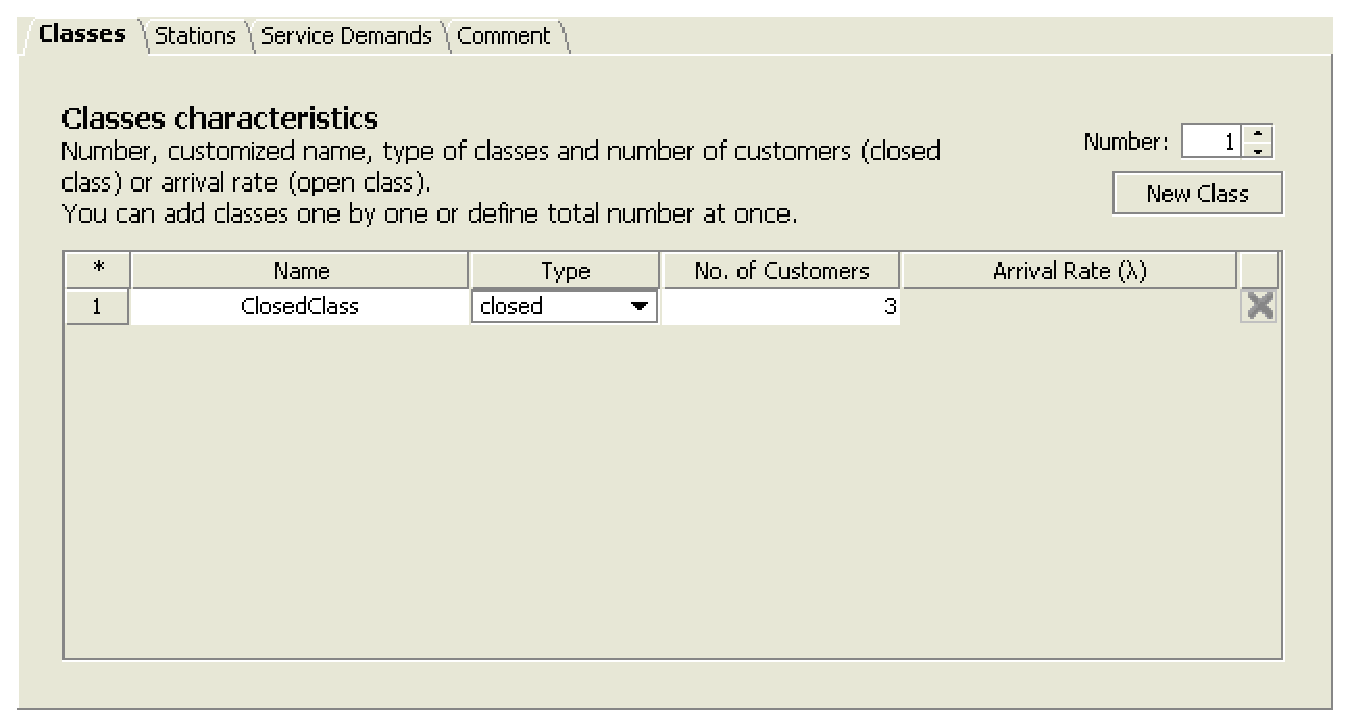
\includegraphics[scale=.5]{img/jmva/example1Class}
    \end{center}
    \caption{Example 1 - input data (Classes Tab)}
    \label{fig:jmva:example1Classes}
\end{figure}

\subsubsection{Step 2 - Stations Tab}
\begin{itemize*}
\item use \texttt{Next $>$} command to switch to \texttt{Stations Tab}
\item digit number 4 into stations number textbox or select number
4 using spin controls or push \emph{New Station} button three times.
Now your model has four \texttt{Load Independent} stations with a
default name
\item if you want you can change station names. Substitute \emph{CPU} for
default name \emph{Station1}, substitute \emph{Disk1} for default
name \emph{Station2}, substitute \emph{Disk2} for default name
\emph{Station3} and substitute \emph{Users} for default name
\emph{Station4}
\item change the type of last inserted station; \emph{Users} station is a
\texttt{Delay (Infinite Server)}
\end{itemize*}

At the end of this step, the \texttt{Stations Tab} should look like
\autoref{fig:jmva:example1Stations}.

\begin{figure}[htbp]
    \begin{center}
        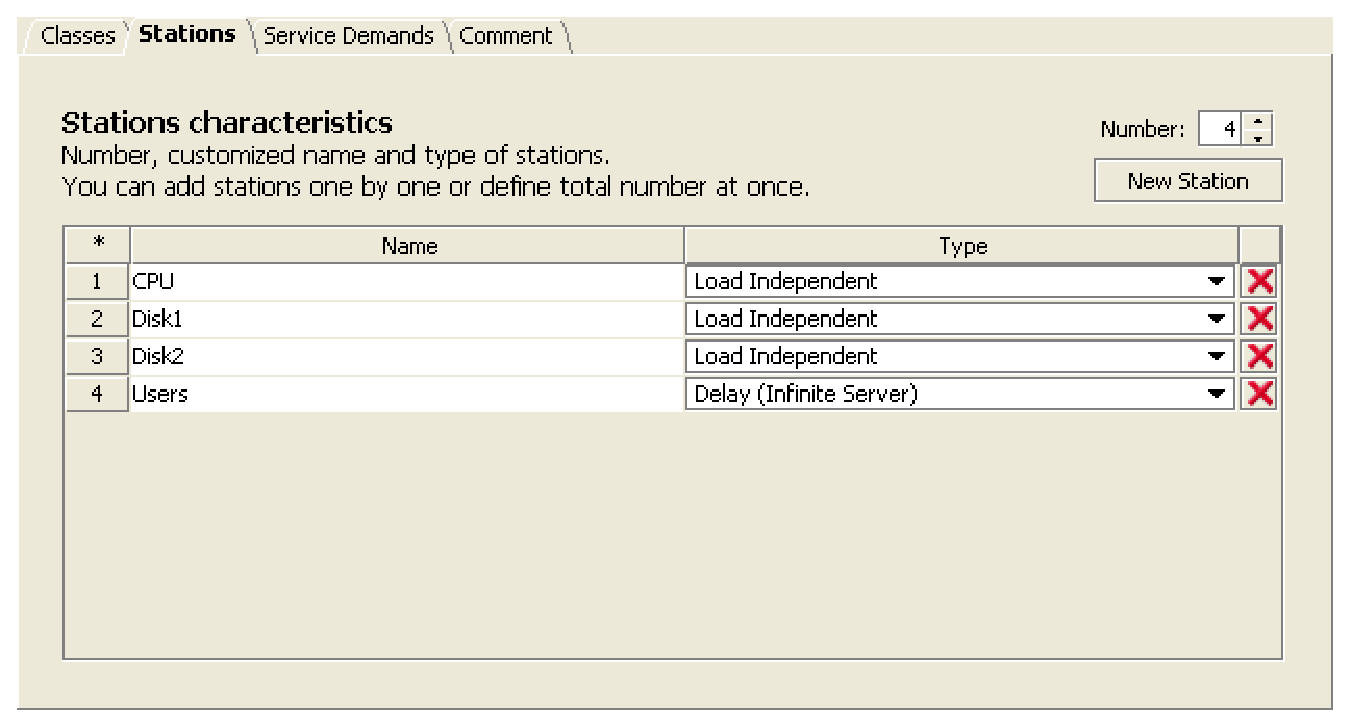
\includegraphics[scale=.5]{img/jmva/example1Stations}
    \end{center}
    \caption{Example 1 - input data (Stations Tab)}
    \label{fig:jmva:example1Stations}
\end{figure}

\subsubsection{Step 3 - Service Times and Visits Tabs}
\begin{itemize*}
\item use \texttt{Next $>$} command to switch to \texttt{Service Demands Tab}
\item press \emph{Service Time and Visit} button as you don't know
the Service Demands of the three stations: in this case Service
Times and number of Visits should be typed. After button pressure,
the \texttt{Service Demands Tab} will be hidden and \texttt{Service
times Tab} and \texttt{Visit Tab} will appear
\item you can input all Service Times in the table.
Remember that Service Time of the \emph{Users} station, of delay
type, is \emph{think time} $Z$, in this case $16$ s
\end{itemize*}

At this point, the \texttt{Service Times Tab} should look like
\autoref{fig:jmva:example1Service}.

\begin{figure}[htbp]
    \begin{center}
        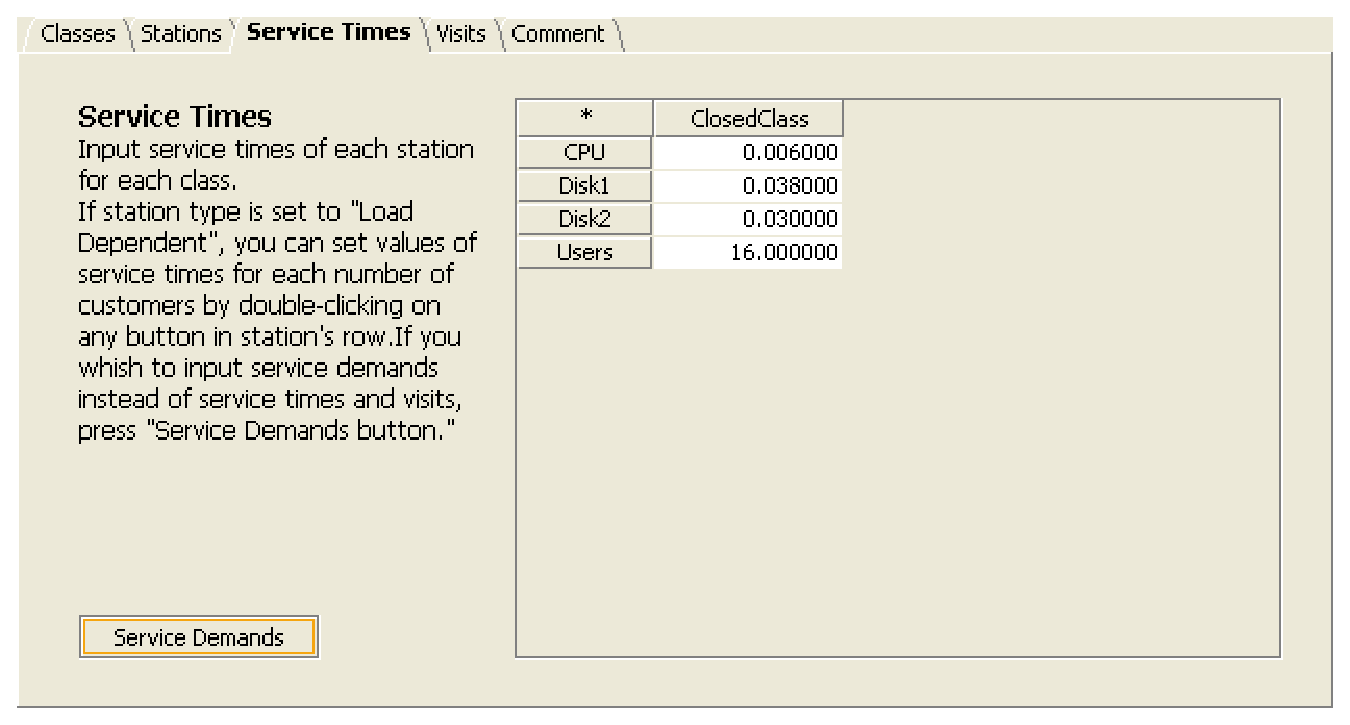
\includegraphics[scale=.5]{img/jmva/example1Service}
    \end{center}
    \caption{Example 1 - input data (Service Times Tab)}
    \label{fig:jmva:example1Service}
\end{figure}

\begin{itemize*}
\item use \texttt{Next $>$} command to switch to \texttt{Visits Tab}
\item input numbers of visits for all centers in the
table. In this case the number of visits of the \emph{Users}, the
infinite server station, is equal to 1 since a customer at the end
of an interaction with the system visits this station.
\end{itemize*}

At the end of this step, the \texttt{Visits Tab} looks like
\autoref{fig:jmva:example1Visits}.

\begin{figure}[htbp]
    \begin{center}
        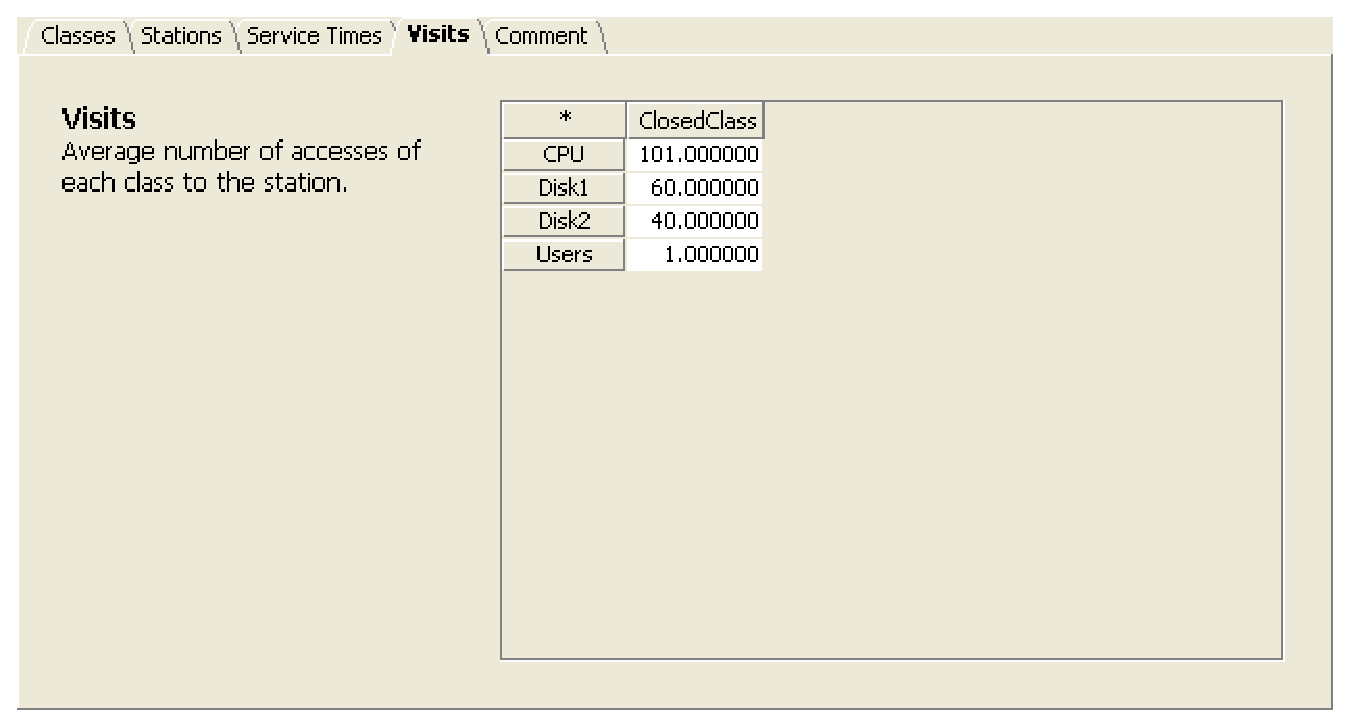
\includegraphics[scale=.5]{img/jmva/example1Visits}
    \end{center}
    \caption{Example 1 - input data (Visits Tab)}
    \label{fig:jmva:example1Visits}
\end{figure}

\subsubsection{Step 4 - Model Resolution}

Use \texttt{Solve} command to start the solution of the input model.
Model results will be displayed in a new window like the one of
\autoref{fig:jmva:example1Throughput}.

\begin{figure}[htbp]
    \begin{center}
        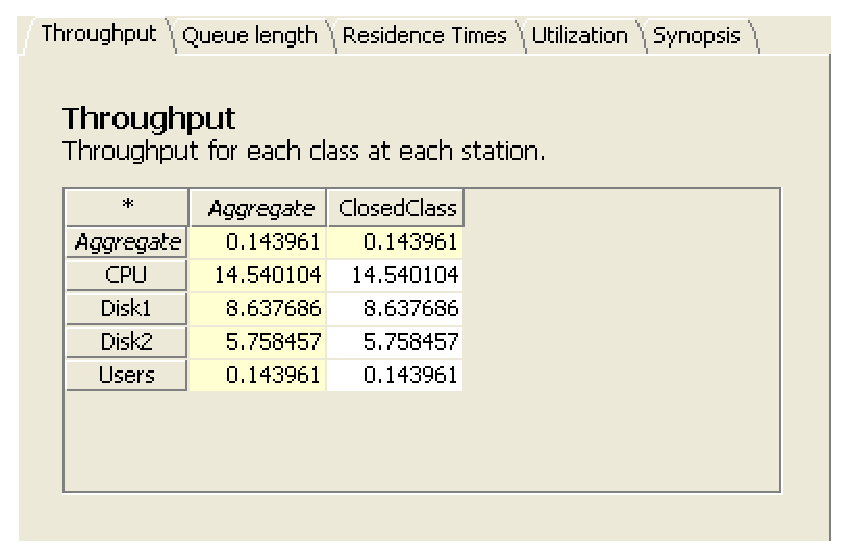
\includegraphics[scale=.5]{img/jmva/example1throughput}
    \end{center}
    \caption{Example 1 - output data (Throughput Tab)}
    \label{fig:jmva:example1Throughput}
\end{figure}

Since we are considering a single-class model, all results in the
column \emph{Aggregate} correspond to the results in the
\emph{ClosedClass} column.

JMVA computes Residence Times $W_k$, Throughputs $X_k$, Queue
lengths $Q_k$ and Utilizations $U_k$ for all stations. The algorithm
begins with the known solution for the network with zero customers,
and iterates on $N$ that, in this example, is three. Note that the
aggregate \emph{Residence Time} is the \emph{System Response Time}
measure and the aggregate \emph{Queue Length} is the average number
of customers in the system.

Using tab selector, you can change tab and see Queue length,
Residence Times, Utilizations and a synopsis panel with a schematic
report of the model (\autoref{fig:jmva:example1results}).

\begin{figure}[htbp]
    \begin{center}
        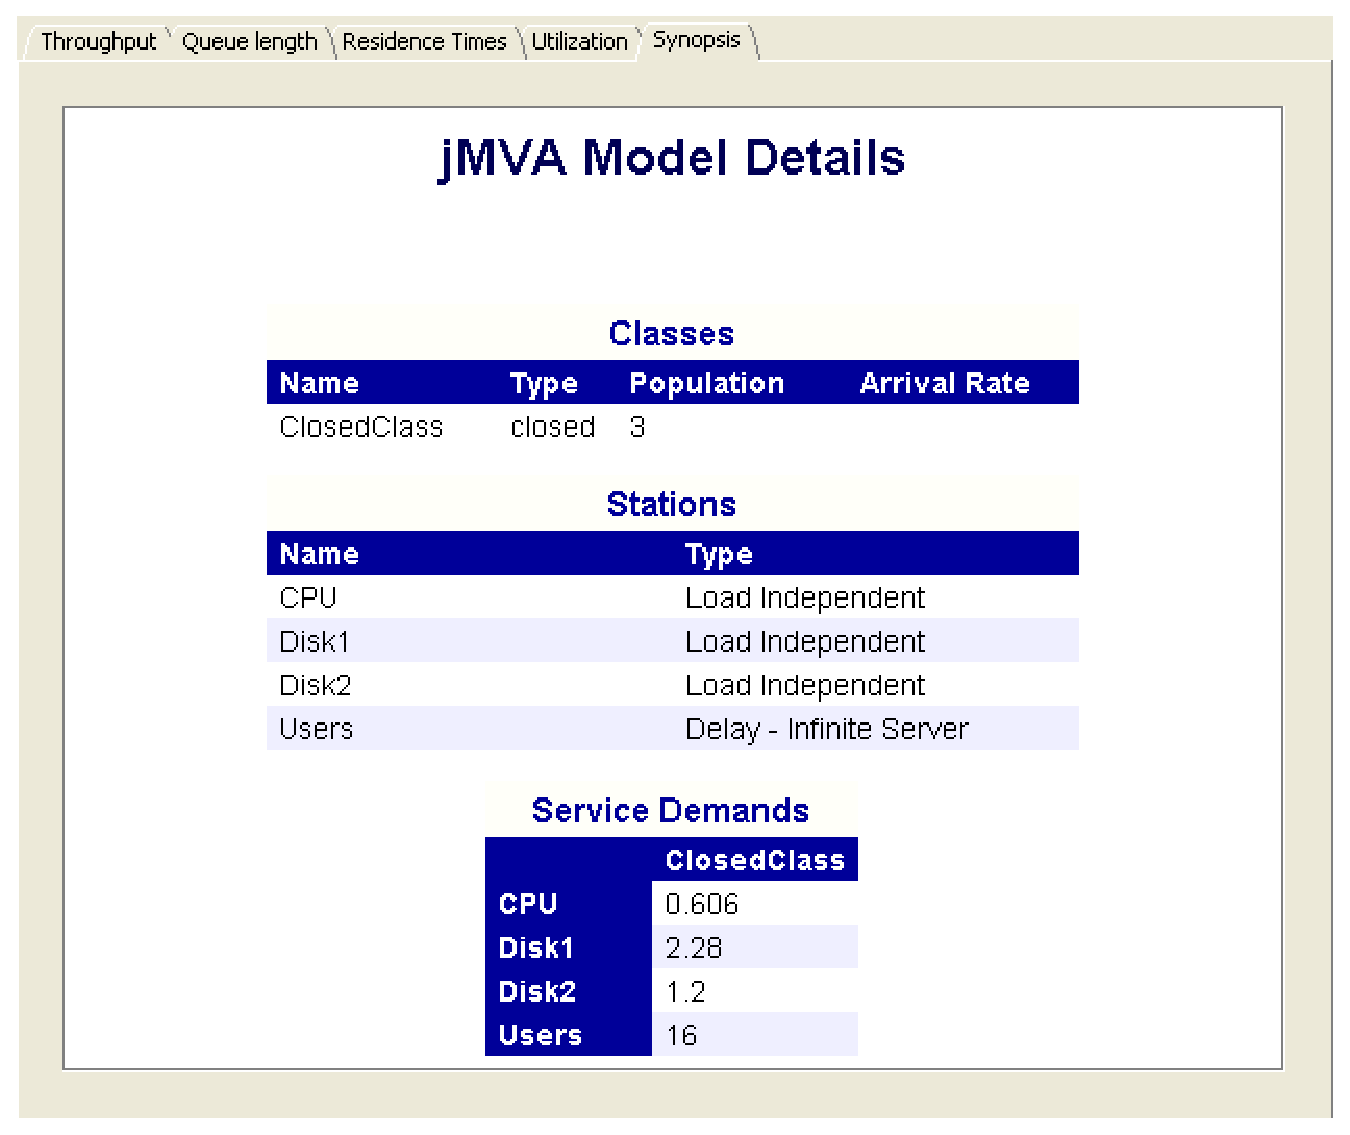
\includegraphics[scale=.5]{img/jmva/example1results}
    \end{center}
    \caption{Example 1 - output data (Synopsis Tab)}
    \label{fig:jmva:example1results}
\end{figure}

The computed performance indices are shown in
\autoref{tab:jmva:example1results}.

\begin{table}[htbp]
\begin{center}
\begin{tabular}{c|r|r|r|r|r|}
& \multicolumn{1}{c|}{Aggregate} & \multicolumn{1}{c|}{CPU} & \multicolumn{1}{c|}{Disk1} & \multicolumn{1}{c|}{Disk2} & \multicolumn{1}{c|}{Users}\\
\hline
Throughput [job/s]& $0.144$ & $14.540$ & $8.637$ & $5.758$ & $0.144$\\
Queue Length [job]& $3.000$ & $0.193$ & $0.410$ & $0.194$ & $2.303$\\
Residence Time [s]& $20.839$ & $0.643$ & $2.847$ & $1.349$ & $16.000$\\
Utilization & \multicolumn{1}{c|}{-} & $0.087$ & $0.328$ & $0.172$ & $2.303$\\
\hline
\end{tabular}
\end{center}
\caption{Example 1 - model outputs} \label{tab:jmva:example1results}
\end{table}


\subsection{Example 2 - A model with two open classes}
\label{sec:jmva:example2} Solve the multiclass open model specified
in \autoref{fig:jmva:Example2topology}.
\begin{figure}[htbp]
    \begin{center}
        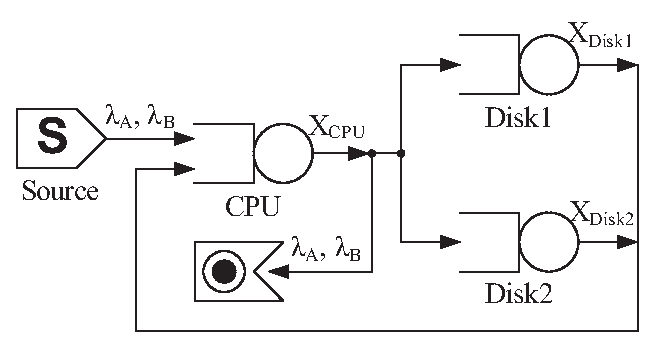
\includegraphics[scale=.65]{img/jmva/example2}
    \end{center}
    \caption{Example 2 - network topology}
    \label{fig:jmva:Example2topology}
\end{figure}
The model is characterized by two open classes $A$ and $B$ with
arrival rate (the workload intensity $\lambda$) respectively of
$\lambda_A = 0.15$ job/s and $\lambda_B=0.32$ job/s. There are three
stations of load independent type, identified with names \emph{CPU},
\emph{Disk1} and \emph{Disk2}. Service times and visits for stations
are shown in \autoref{tab:jmva:example2ServTimes} and
\autoref{tab:jmva:example2Visits}.

\begin{table}[htbp]
\begin{center}
\begin{tabular}{c|r|r|r|r|}
& \multicolumn{1}{c|}{CPU} & \multicolumn{1}{c|}{Disk1} & \multicolumn{1}{c|}{Disk2} \\
\hline
Class $A$ [s]& $0.006$ & $0.038$ & $0.030$ \\
Class $B$ [s]& $0.014$ & $0.062$ & $0.080$ \\
\hline
\end{tabular}
\end{center}
\caption{Example 2 - service times}
\label{tab:jmva:example2ServTimes}
\end{table}

\begin{table}[htbp]
\begin{center}
\begin{tabular}{c|r|r|r|r|}
& \multicolumn{1}{c|}{CPU} & \multicolumn{1}{c|}{Disk1} & \multicolumn{1}{c|}{Disk2} \\
\hline
Class $A$ & $101.0$ & $60.0$ & $40.0$ \\
Class $B$ & $44.0$ & $16.0$ & $27.0$ \\
\hline
\end{tabular}
\end{center}
\caption{Example 2 - number of visits}
\label{tab:jmva:example2Visits}
\end{table}

Since this model is similar to the network of
\autoref{fig:jmva:Example1topology} solved in
\autoref{sec:jmva:example1}, we will show how to easily create it
from a saved copy of Example~1:
\begin{enumerate*}
    \item Open the saved instance of Example~1 model
    \item Go to \texttt{Classes Tab}, change \emph{ClosedClass} name
    to \emph{A}, change its type to \texttt{Open} and set its arrival
    rate to $\lambda_A = 0.15$ job/s.
    \item Click on \emph{New Class} button, sets name of new class to
    \emph{B}, change its type to \texttt{Open} and set its arrival
    rate to $\lambda_B = 0.32$ job/s.
    \item Go to \texttt{Stations Ta}b and remove \emph{Users} delay
    center.
    \item Go to \texttt{Service Times Tab} and sets service times for
    Class $B$ according to \autoref{tab:jmva:example2ServTimes}.
    \item Go to \texttt{Visits Tab} and sets visits for
    Class $B$ according to \autoref{tab:jmva:example2Visits}.
    \item Select \texttt{Solve} action.
\end{enumerate*}

The \texttt{Synopsis Tab} with a schematic report of the model
created is shown on \autoref{fig:jmva:example2results}, while the
computed performance indices of this model are shown in
\autoref{tab:jmva:example2results}.

\begin{figure}[htbp]
    \begin{center}
        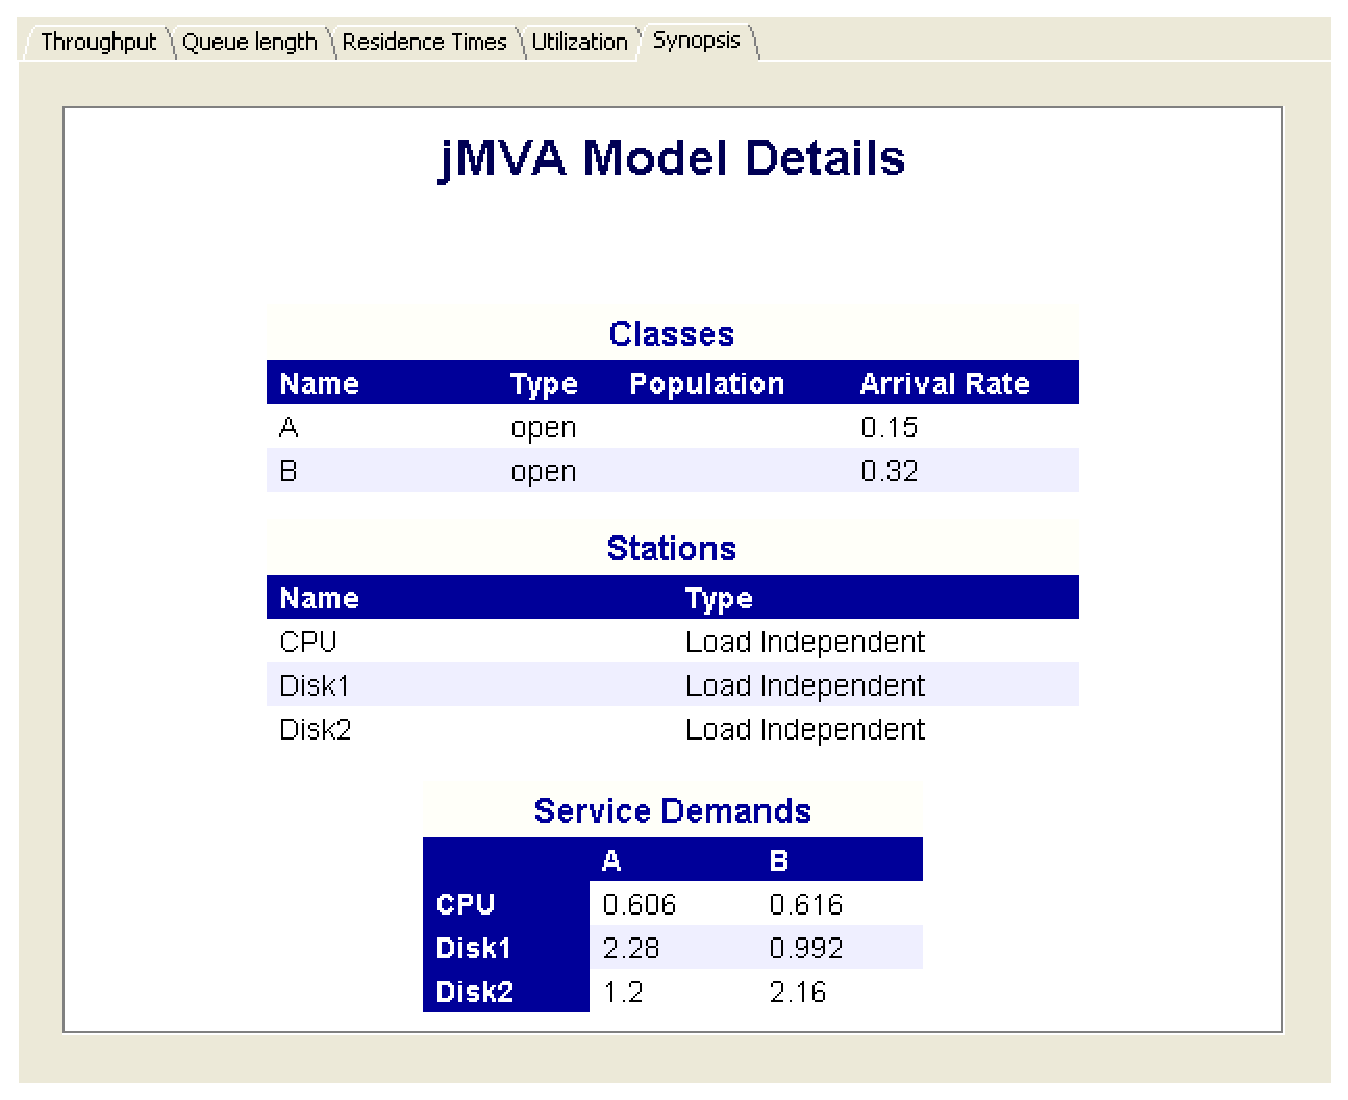
\includegraphics[scale=.5]{img/jmva/example2results}
    \end{center}
    \caption{Example 2 - output data (Synopsis Tab)}
    \label{fig:jmva:example2results}
\end{figure}

\begin{table}[htbp]
\begin{center}
\begin{tabular}{c|r|r|r|r|}
&\multicolumn{4}{c|}{Class $A$}\\
& \multicolumn{1}{c|}{Aggregate} & \multicolumn{1}{c|}{CPU} & \multicolumn{1}{c|}{Disk1} & \multicolumn{1}{c|}{Disk2}\\
\hline Throughput [job/s]& $0.150$ & $15.150$ & $9.000$ & $6.000$\\
Queue Length [job]& $2.529$ & $0.128$ & $1.004$ & $1.398$\\
Residence Time [s]& $16.863$ & $0.851$ & $6.695$ & $9.317$\\
Utilization & \multicolumn{1}{c|}{-} & $0.091$ & $0.342$ & $0.180$\\
\hline \multicolumn{5}{c}{ }\\
\multicolumn{5}{c}{ }\\
&\multicolumn{4}{c|}{Class $B$}\\
& \multicolumn{1}{c|}{Aggregate} & \multicolumn{1}{c|}{CPU} & \multicolumn{1}{c|}{Disk1} & \multicolumn{1}{c|}{Disk2}\\
\hline Throughput [job/s]& $0.320$ & $14.080$ & $5.120$ & $8.640$\\
Queue Length [job]& $6.575$ & $0.277$ & $0.932$ & $5.366$\\
Residence Time [s]& $20.548$ & $0.865$ & $2.913$ & $16.770$\\
Utilization & \multicolumn{1}{c|}{-} & $0.197$ & $0.317$ & $0.691$\\
\hline
\end{tabular}

\end{center}
\caption{Example 2 - model outputs} \label{tab:jmva:example2results}
\end{table}

\subsection{Example 3 - A model with a load dependent station}
\label{sec:jmva:example3} The network is shown in
\autoref{fig:jmva:Example3topology}.
\begin{figure}[htbp]
    \begin{center}
        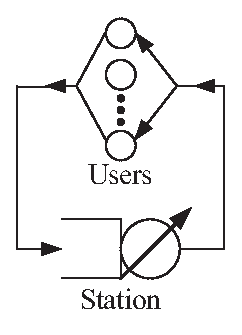
\includegraphics[scale=.65]{img/jmva/example3}
    \end{center}
    \caption{Example 3 - network topology}
    \label{fig:jmva:Example3topology}
\end{figure}
It comprises only two stations: one is of delay type (named
\emph{Users}) and the other is a load dependent station (named
\emph{Station}). This model has one closed class only with $N=8$
customers. The user's \emph{think time} is $Z = 21$ s, while the
service demands for the load dependent \emph{Station}, shown in
\autoref{tab:jmva:example3ServDemands}, are function of $n$: number
of customers in the station ($D(n) = n + 1/n$).

\begin{table}[htbp]
\begin{center}
\begin{tabular}{c|c|c|c|c|c|c|c|c|}
$n$ & $1$ & $2$ & $3$ & $4$ & $5$ & $6$ & $7$ & $8$\\
\hline
$D(n)$ [s] & $2.00$ & $2.50$ & $3.33$ & $4.25$ & $5.20$ & $6.17$ & $7.14$ & $8.13$ \\
\hline
\end{tabular}
\end{center}
\caption{Example 3 - service demands for \emph{Station}, a
load-dependent service center} \label{tab:jmva:example3ServDemands}
\end{table}

\subsubsection{Step 1 - Classes Tab}

The instructions that are the same given in Step 1 of
\autoref{sec:jmva:example1}; in this case $N$ must be 8.

\subsubsection{Step 2 - Stations Tab}

The instructions are given in Step 2 of \autoref{sec:jmva:example1};
in this case the model has two stations: a Load Dependent station
and a Delay Center.

\subsubsection{Step 3 - Service Demands Tab}

\begin{enumerate*}
\item use \texttt{Next $>$} command to switch to \texttt{Service Demands Tab}
\item double-click on cell with text \emph{LD Setting\dots}
to open the editor of load dependent service demands in a separate
window, shown in \autoref{fig:jmva:example3ldBefore}.
\item it is not mandatory to insert all values one-by-one. You can
click or drag to select cells, enter the expression $n + 1/n$ into
the textbox at the bottom of the window and click the
\emph{Evaluate} button.
\item at the end of this phase, editor window looks like
\autoref{fig:jmva:example3ldAfter}. Now you may press \emph{OK}
button to confirm changes and return to JMVA main window.
\end{enumerate*}

\begin{figure}[htbp]
    \begin{center}
        \includegraphics[scale=.5]{img/jmva/example3ldBefore}
    \end{center}
    \caption{Example 3 - editor for the description of service
    demands for a load dependent station corresponding to the different number of
    customers before the parametrization}
    \label{fig:jmva:example3ldBefore}
\end{figure}

\begin{figure}[htbp]
    \begin{center}
        \includegraphics[scale=.5]{img/jmva/example3ldAfter}
    \end{center}
    \caption{Example 3 - editor for the description of service
    demands for a load dependent station. In this case an arithmetic function
    has been defined: $S(n)=n+1/n$}
    \label{fig:jmva:example3ldAfter}
\end{figure}

\subsubsection{Step 4 - Model Resolution}

Use \texttt{Solve} command to resolve the model, results are shown
in \autoref{tab:jmva:example4results}.

\begin{table}[htbp]
\begin{center}
\begin{tabular}{c|r|r|r|r|r|}
& \multicolumn{1}{c|}{Aggregate} & \multicolumn{1}{c|}{Station} & \multicolumn{1}{c|}{Users}\\
\hline
Throughput [job/s] & $0.234$ & $0.234$ & $0.234$ \\
Queue Length [job]& $8.000$ & $3.080$ & $4.920$ \\
Residence Time [s]& $34.149$ & $13.149$ & $21.000$ \\
Utilization & \multicolumn{1}{c|}{-} & $0.810$ & $0.973$ \\
\hline
\end{tabular}
\end{center}
\caption{Example 4 - model outputs} \label{tab:jmva:example4results}
\end{table}

\subsection{Example 4 - A model with one open and one closed class}
\label{sec:jmva:example4}

The mixed queueing network model is shown in
\autoref{fig:jmva:Example4topology}.
\begin{figure}[htbp]
    \begin{center}
        \includegraphics[scale=.65]{img/jmva/example4}
    \end{center}
    \caption{Example 4 - network topology}
    \label{fig:jmva:Example4topology}
\end{figure}
Workload intensities: the open class has an arrival rate $\lambda =
1$ job/s, the closed class has a customers number $N = 57$. Service
demands are shown in \autoref{tab:jmva:example4ServDemands}.

\begin{table}[htbp]
\begin{center}
\begin{tabular}{c|r|r|r|r|}
& \multicolumn{1}{c|}{Station1} & \multicolumn{1}{c|}{Station2} & \multicolumn{1}{c|}{Station3} \\
\hline
OpenClass [s]& $0.5$ & $0.8$ & $0.6$ \\
ClosedClass [s]& $10.0$ & $4.0$ & $8.0$ \\
\hline
\end{tabular}
\end{center}
\caption{Example 4 - service demands}
\label{tab:jmva:example4ServDemands}
\end{table}

\subsubsection{Step 1 - Classes Tab}

Follow the instructions of Step~1 in the previous examples; the
\texttt{Classes Tab} is shown in \autoref{fig:jmva:example4Class}.

\begin{figure}[htbp]
    \begin{center}
        \includegraphics[scale=.5]{img/jmva/example4Class}
    \end{center}
    \caption{Example 4 - Class Tab}
    \label{fig:jmva:example4Class}
\end{figure}

\subsubsection{Step 2 - Stations Tab}

Follow the instructions of Step~2 in the previous examples; in this
case the model has three Load Independent stations (see
\autoref{fig:jmva:example4Stations}).

\begin{figure}[htbp]
    \begin{center}
        \includegraphics[scale=.5]{img/jmva/example4Stations}
    \end{center}
    \caption{Example 4 - Stations Tab}
    \label{fig:jmva:example4Stations}
\end{figure}

\subsubsection{Step 3 - Service Demands Tab}

Follow the instructions of Step~3 in the previous examples and
define service demands for both classes as illustrated in
\autoref{tab:jmva:example4ServDemands} (see
\autoref{fig:jmva:example4Services}).

\begin{figure}[htbp]
    \begin{center}
        \includegraphics[scale=.5]{img/jmva/example4Services}
    \end{center}
    \caption{Example 4 - Service Demands Tab}
    \label{fig:jmva:example4Services}
\end{figure}

\subsubsection{Step 4 - Model Solution}
Use \texttt{Solve} command. Results can be verified by computing the
\emph{equivalent model}, where the open class ``slows down'' the
closed class by subtracting utilization to it:

\begin{eqnarray*}
D_{1}^{eq}&=&\frac{D_{1,ClosedClass}}{1- \lambda * D_{1,OpenClass}} = 20 s\\
D_{2}^{eq}&=&\frac{D_{2,ClosedClass}}{1- \lambda * D_{2,OpenClass}} = 20 s\\
D_{3}^{eq}&=&\frac{D_{3,ClosedClass}}{1- \lambda * D_{3,OpenClass}} = 20 s\\
\end{eqnarray*}

MVA algorithm is used to solve the equivalent closed model. The
number of customers of the closed class is $57$, and the exact MVA
technique should require the solution of other $56$ models with
smaller population. In this particular case, the formula used to
compute the throughput can be simplified because the Service Demands
are all equals:

\begin{eqnarray*}
X^{eq}(N)&=&\frac{N}{\sum_{k=1}^{3} D_{k}^{eq} + \sum_{k=1}^{3}
\left[D_{k}^{eq}*Q_{k}^{eq}(N-1)\right]}\\
&=&\frac{N}{60 + 20*\sum_{k=1}^{3}
Q_{k}^{eq}(N-1)}\\
&=&\frac{N}{60 + 20*(N-1)}\\
\\
\\
X^{eq}(57)&=&0.048305 \textrm{ job/s}
\end{eqnarray*}

So the throughput measure for the closed class is $X_{ClosedClass} =
X^{eq} = 0.048305$ job/s while the throughput for the open class
coincide with its arrival rate $X_{OpenClass} = \lambda$. As visits
were not specified, they have been considered equal to one: that's
why throughput is equal at each station for each class (see
\autoref{fig:jmva:example4Throughput}), i.e. the solved model
consists of 3 stations that are sequentially connected with
feedback.

\begin{figure}[htbp]
    \begin{center}
        \includegraphics[scale=.5]{img/jmva/example4Throughput}
    \end{center}
    \caption{Example 4 - throughput}
    \label{fig:jmva:example4Throughput}
\end{figure}

Queue lenghts can be computed with the following formulas:
\begin{eqnarray*}
Q_{k,ClosedClass}(N)&=&Q_k^{eq}(N)\\
Q_{k,OpenClass}(N)&=&\frac{\lambda*D_{k,OpenClass}*\left[1+Q_{k,ClosedClass}(N)\right]}{1-\lambda*D_{k,OpenClass}}
\end{eqnarray*}

And the results will be equal to the ones shown in
\autoref{fig:jmva:example4Queue}.

\begin{figure}[htbp]
    \begin{center}
        \includegraphics[scale=.5]{img/jmva/example4Queue}
    \end{center}
    \caption{Example 4 - queue lengths}
    \label{fig:jmva:example4Queue}
\end{figure}

\subsection{Example 5 - Find optimal Population Mix values}
\label{sec:jmva:example5} Perform a what-if analysis to find the
value of population mix that will maximize \texttt{System
Throughput} and minimize \texttt{System Response Time} in the model
shown in \autoref{fig:jmva:Example5topology}.
\begin{figure}[htbp]
    \begin{center}
        \includegraphics[scale=.65]{img/jmva/example5}
    \end{center}
    \caption{Example 5 - network topology}
    \label{fig:jmva:Example5topology}
\end{figure}
This model has two closed classes (named \emph{Class1} and
\emph{Class2}) with a total population of $N=20$ and three load
independent stations (named \emph{Station1}, \emph{Station2} and
\emph{Station3}) with the service demands shown in
\autoref{tab:jmva:example5ServDemands}.

\begin{table}[htbp]
\begin{center}
\begin{tabular}{c|r|r|r|r|}
& \multicolumn{1}{c|}{Station1} & \multicolumn{1}{c|}{Station2} & \multicolumn{1}{c|}{Station3} \\
\hline
Class1 [s]& $1.0$ & $5.0$ & $1.0$ \\
Class2 [s]& $5.0$ & $1.0$ & $5.0$ \\
\hline
\end{tabular}
\end{center}
\caption{Example 5 - service demands}
\label{tab:jmva:example5ServDemands}
\end{table}

\subsubsection{Step 1 - Classes Tab}

Follow the instructions of Step~1 in the previous examples; as we
will change population mix, initial allocation of the $N=20$ jobs is
irrelevant. For example we can allocate $N_1=10$ jobs to
\emph{Class1} and $N_2=10$ jobs to \emph{Class2}. The
\texttt{Classes Tab} is shown in \autoref{fig:jmva:example5Class}.

\begin{figure}[htbp]
    \begin{center}
        \includegraphics[scale=.5]{img/jmva/example5Class}
    \end{center}
    \caption{Example 5 - Class Tab}
    \label{fig:jmva:example5Class}
\end{figure}

\subsubsection{Step 2 - Stations Tab}

Follow the instructions of Step~2 in the previous examples; in this
case the model has three Load Independent stations (see
\autoref{fig:jmva:example5Stations}).

\begin{figure}[htbp]
    \begin{center}
        \includegraphics[scale=.5]{img/jmva/example5Stations}
    \end{center}
    \caption{Example 5 - Stations Tab}
    \label{fig:jmva:example5Stations}
\end{figure}

\subsubsection{Step 3 - Service Demands Tab}

Follow the instructions of Step~3 in the previous examples and
define service demands for both classes as illustrated in
\autoref{tab:jmva:example5ServDemands} (see
\autoref{fig:jmva:example5Services}).

\begin{figure}[htbp]
    \begin{center}
        \includegraphics[scale=.5]{img/jmva/example5Services}
    \end{center}
    \caption{Example 5 - Service Demands Tab}
    \label{fig:jmva:example5Services}
\end{figure}

\subsubsection{Step 4 - What-if Tab}
\begin{enumerate*}
    \item use \texttt{Next $>$} command to switch to \texttt{What-if Tab}
    \item Select \texttt{Population Mix} as a \emph{control parameter} of
    the analysis in the combo box, several fields will be shown below.
    \item \emph{Class1} is already selected, by default, as reference class for the what-if
    analysis. This means that $\beta_i$ values in \texttt{From} and
    \texttt{To} fields are referred to \emph{Class1}.
    \item By default, JMVA suggests the minimum allowed value of $\beta_1$
    in the \texttt{From} field and its the maximum value in the \texttt{To}
    field\footnote{Since it is requested that one class has at least one job and customer
    number must be integer, the minimum value is $1 / N$ and the maximum value is $(N-1)/N$.}.
    Since we want to find the optimal value in the entire
    interval, we leave this unchanged.
    \item we want to perform the maximum number of allowed
    executions, so we enter a big number in the \texttt{Steps} field ($100$ for
    example). JMVA will automatically calculate the maximum number
    of allowed executions provided that number of customers for each
    class must be an integer and will report $19$.
\end{enumerate*}
At the end of this phase, the What-if Tab will look like
\autoref{fig:jmva:example5Whatif}.

\begin{figure}[htbp]
    \begin{center}
        \includegraphics[scale=.5]{img/jmva/example5Whatif}
    \end{center}
    \caption{Example 5 - What-if Tab}
    \label{fig:jmva:example5Whatif}
\end{figure}


\subsubsection{Step 5 - Model Solution}
Use \texttt{Solve} command. In the \texttt{Graphical Results Tab}
select \texttt{System Response Time} and \texttt{System Throughput}
as \emph{Performance Index}
(\autoref{fig:jmva:example5SystemResponse} and
\autoref{fig:jmva:example5SystemThroughput}). Zooming on the plot,
allows to identify the maximum value of System Throughput ($0.32$
job/s) and the minimum value of System Response Time ($62.50$ s).
They both corresponds to the execution with population mix $\beta_1
= 0.40$ for \emph{Class1}, which means that the optimal population
values are $N_1 = 8$ and $N_2 = 12$.

\begin{figure}[htbp]
    \begin{center}
        \includegraphics[scale=.5]{img/jmva/example5SystemResponse}
    \end{center}
    \caption{Example 5 - System Response Time}
    \label{fig:jmva:example5SystemResponse}
\end{figure}

\begin{figure}[htbp]
    \begin{center}
        \includegraphics[scale=.5]{img/jmva/example5SystemThroughput}
    \end{center}
    \caption{Example 5 - System Throughput}
    \label{fig:jmva:example5SystemThroughput}
\end{figure}

%
% This document is free; you can redistribute it and/or modify
% it under the terms of the GNU General Public License as published by
% the Free Software Foundation; either version 2 of the License, or
% (at your option) any later version.
%
% This document is distributed in the hope that it will be useful, but
% WITHOUT ANY WARRANTY; without even the implied warranty of
% MERCHANTABILITY or FITNESS FOR A PARTICULAR PURPOSE.  See the GNU
% General Public License for more details.
%
% You should have received a copy of the GNU General Public License
% along with this document; if not, write to the Free Software
% Foundation, Inc., 51 Franklin Street, Fifth Floor, Boston, MA
% 02110-1301, USA.
%
% Author: Bertoli Marco
%
\chapter{JSIM}
\label{cha:jsim}
\section{Overview}
JSIM analyzes open, closed and mixed queueing networks using a discrete-event simulator \cite{DESimulation}. A sequence of \emph{wizard} windows helps specifying network properties. The simulation engine supports several probability distributions for characterizing service and inter-arrival times, e.g., exponential, hyperexponential, uniform, Erlang and Pareto. Random number generation is based on the Mersenne twister engine \cite{Mersenne}. It is also possible to reproduce a given sequence of random numbers, in order to simulate real workloads from collected
log files. Load-dependent strategies using arbitrary functions of the current queue-length can be specified.

JSIM supports state-independent routing strategies, e.g., Markovian or round robin, as well as state-dependent strategies, e.g., routing to the server with minimum utilization, or
with the shortest response time, or with minimum queue length.

Performance indices like throughputs, utilizations, response times, residence times, queue-lengths are evaluated. The simulation engine supports several extended features
not allowed in product-form models, namely, finite capacity regions (i.e., blocking), fork-join servers, and priority classes. Finite capacity regions may include either shared
or class-specific population constraints. 

The analysis of simulation results employs on-line transient detection techniques based on spectral analysis \cite{Spectral}. What-if analysis, where a sequence of simulations is run for different
values of parameters, are also possible.

\subsection{Starting the alphanumeric simulator}
Selecting \includegraphics[scale=.5]{img/JSIMIcon} button on the
starting screen, \autoref{fig:jsim:Classes} window shows up.
\begin{figure}[htb]
    \begin{center}
        \includegraphics[width=300pt]{img/jsim/classes}
    \end{center}
    \caption{Classes Panel}
    \label{fig:jsim:Classes}
\end{figure}
Each JSIM panel is organized to be compliant with a given layout, shown in \autoref{fig:jsim:panellayout}, 
\begin{figure}[tb]
    \begin{center}
        \includegraphics[width=300pt]{img/jsim/panelLayout}
    \end{center}
    \caption{Layout of JSIM panels}
    \label{fig:jsim:panellayout}
\end{figure}
where the following main areas can be identified:


%
% This document is free; you can redistribute it and/or modify
% it under the terms of the GNU General Public License as published by
% the Free Software Foundation; either version 2 of the License, or
% (at your option) any later version.
%
% This document is distributed in the hope that it will be useful, but
% WITHOUT ANY WARRANTY; without even the implied warranty of
% MERCHANTABILITY or FITNESS FOR A PARTICULAR PURPOSE.  See the GNU
% General Public License for more details.
%
% You should have received a copy of the GNU General Public License
% along with this document; if not, write to the Free Software
% Foundation, Inc., 51 Franklin Street, Fifth Floor, Boston, MA
% 02110-1301, USA.
%
% Author: Carlo Gimondi
%
\chapter{JABA (Asymptotic Bound Analysis)}
\label{cha:jaba}
\section{Overview}
Product-form queueing network models are used for modelling the
performance of many type of systems, from large computing
infrastructures to distributed applications. The complexity of
modern systems makes the application of exact solution techniques,
such as the convolution algorithm or the MVA, prohibitively
expensive in terms of computational resource requirements. Also
approximate solution techniques become less accurate or more
expensive with the growing complexity of the models. The
alternative is represented by \emph{asymptotic} techniques that
can efficiently determine asymptotic values for several
performance indices such as throughput, response time and queue
lengths. The asymptotic techniques are particularly useful in
tuning studies where one needs to evaluate the performance gains
of different tuning alternatives. The key to determine the
asymptotic performances is the knowledge of the queueing center(s)
with the highest utilization, i.e. the \emph{bottleneck
station(s)}. Multiclass models can exhibit multiple simultaneous
bottlenecks depending of the population mix. While identifying the
bottleneck stations under a single-class workload is a
well-established practice, no simple methodology for multiclass
models has yet been found. JABA provides such a technique, called
Polyhedral Analysis, using convex polytopes based approach
presented in \cite{polytopes}.

Among the no-bottleneck station, we distinguish two different
centers: \emph{dominated} and \emph{masked-off} stations. This
distinction is important since the \emph{masked-off} stations,
despite having lower utilization than the bottleneck center(s),
may still exhibit the largest queue-length and hence the highest
response times. \emph{Dominated} stations, instead, typically play
a marginal role in determining system performance, and have always
the smallest utilization and queue-lengths.


\subsection{Starting the alphanumeric JABA solver}
Selecting \includegraphics[scale=.5]{img/JABAIcon} button on the
starting screen, \autoref{fig:jaba:Classes} the JABA window shows up.
\begin{figure}[htbp]
    \begin{center}
        \includegraphics[scale=.5]{img/jaba/classes}
    \end{center}
    \caption{Classes tab}
    \label{fig:jaba:Classes}
\end{figure}

Three main areas are shown:
\begin{description*}
\item[Menu :] it is organized into three groups of functions. To use a
menu, click on the menu heading and choose the appropriate option.
For the description of menu entries, see \autoref{sec:jaba:Menu}
\item[Toolbar :] contains some buttons to speed up access to JABA functions
(e.g. New model, Open, Save\dots See \autoref{sec:jaba:Menu} for
details). If you move the mouse pointer over a button a tooltip will
be shown up.
\item[Page Area :] this is the core of the window. All JABA parameters are grouped in
different tabs. You can modify only a subset of them by selecting
the proper tab, as will be shown later.
\end{description*}

\section{Model definition}
Models with two or three customer classes provide estimates of wich stations are potential bottleneck.
For a brief description of basic terminology please refer to \autoref{cha:glossary}.

The workload is characterized for each station by the service
demands of every customer class.
Al least JABA works with 2 classes of custumers therefore a matrix of
service demands is required \cite{Lazowska}.

\subsection{Defining a new model}
To define a new model select toolbar button
\includegraphics[scale=.8]{img/jaba/new} or the \emph{New} command
from \emph{File} menu. The following parameters must be defined:
\begin{enumerate*}
\item \texttt{Classes}
\item \texttt{Stations} (service centers)
\item \texttt{Service demands} (or Service Times and Visits)
\item Optional short \texttt{Comment}
\end{enumerate*}

The execution of JABA produces the following graph:

\begin{itemize*}
\item Saturation Sector - Graphics
\item Convex Hull - Graphics
\end{itemize*}

\noindent And a textual report about the saturation sectors:
\begin{itemize*}
\item Saturation Sectors - Text
\end{itemize*}

\subsubsection{Input tabs}
As shown in \autoref{fig:jaba:Classes}, the parameters that
must be entered in order to define a new model are divided in four
tabs: \texttt{Classes}, \texttt{Stations}, \texttt{Service Demands}
and \texttt{Comment}.

The number of tabs become five, if you click  \emph{Service Times and
Visits} button in \texttt{Service Demands Tab}. As will be discussed
in \autoref{sec:jaba:ServiceDemand}, the \texttt{Service Demands
Tab} will be hidden and it will appear \texttt{Service Times Tab}
and \texttt{Visit Tab}. You can navigate across tabs:
\begin{itemize*}
\item using sequential wizard buttons, if enabled, at the bottom of
the window (\autoref{fig:jaba:Wizardbuttons})
\item using sequential buttons located in menu
\item using the tab selector, clicking on the corresponding
tab (\autoref{fig:jaba:Tabselector})
\end{itemize*}

\begin{figure}[htbp]
    \begin{center}
        \includegraphics[scale=.5]{img/jaba/wizBut}
    \end{center}
    \caption{Wizard buttons}
    \label{fig:jaba:Wizardbuttons}
\end{figure}

\begin{figure}[htbp]
    \begin{center}
        \includegraphics[scale=.5]{img/jaba/tabSel}
    \end{center}
    \caption{Tab selector}
    \label{fig:jaba:Tabselector}
\end{figure}

\subsection{Classes Tab}
An example screenshot of this tab can be seen in
\autoref{fig:jaba:Classes}. This tab allows to set the number of custumer classes.
It's possible to set two or three clesses.

The number of classes in the model can be specified in the
corresponding input area, shown in \autoref{fig:jaba:ClassNum} and
can be modified using the keyboard or the spin controls.
\begin{figure}[htbp]
    \begin{center}
        \includegraphics[scale=.5]{img/jaba/classNum}
    \end{center}
    \caption{Number of classes}
    \label{fig:jaba:ClassNum}
\end{figure}

Using the delete button
\includegraphics[scale=.6]{img/jaba/x} associated to a specific
class, a class can be removed provided that there will be at least
one class after the deletion. Similar result may be obtained using
spin controls, decreasing classes number; in this case last inserted
class will be removed.

Default class names are \emph{Class1}, \emph{Class2}, \dots
\emph{ClassN}. The model can be personalized by changing these names.

\subsection{Stations Tab}
The number of stations of the model can be specified in the
corresponding input area (\autoref{fig:jaba:stationNum}) and can be
modified using the keyboard or the spin controls.

\begin{figure}[htbp]
    \begin{center}
        \includegraphics[scale=.5]{img/jaba/stationNum}
    \end{center}
    \caption{Number of stations}
    \label{fig:jaba:stationNum}
\end{figure}

Using the delete button
\includegraphics[scale=.6]{img/jaba/x} associated to a specific
station, a station can be removed provided that there will be at
least one station after the deletion. Similar result may be obtained decreasing stations number using spin controls; in this case last inserted station will be removed.

Default station names are \emph{Station1}, \emph{Station2}, \dots
\emph{StationN}. In order to personalize your model, you can change
and give names other than default ones.

In \autoref{fig:jaba:stations} there is only one station with
default name \emph{Station4} and there are three stations with
personalized names: \emph{CPU}, \emph{Disk1} and \emph{Disk2}.

\begin{figure}[htbp]
    \begin{center}
        \includegraphics[scale=.5]{img/jaba/4stations}
    \end{center}
    \caption{Defining the stations name}
    \label{fig:jaba:stations}
\end{figure}


\subsection{Service Demands, Service Times and Visits Tabs}
\label{sec:jaba:ServiceDemand} Service Demands can be defined in two
ways:
\begin{itemize*}
\item directly, by entering Service Demands ($D_{kc}$)
\item indirectly, by entering Service Times ($S_{kc}$) and Visits ($V_{kc}$)
\end{itemize*}

Service demand $D_{kc}$ is the total service requirement, that is
the average amount of time that a customer of class $c$ spends in
service at station $k$ during one interaction with the system, i.e.
it's complete execution. Service time $S_{kc}$ is the average time
spent by a customer of class $c$ at station $k$ for a single visit
at that station while $V_{kc}$ is the average number of visits at
that resource for each interaction with the system.

Remember that $D_{kc} = V_{kc} * S_{kc}$ so it's simple to compute
service demands matrix starting from service times and visits
matrixes. Inverse calculation is performed with the following
algorithm:
\[
V_{kj} = \left\{
\begin{array}{ccl} 1 & \textrm{if} & D_{kc} > 0 \\
0 & \textrm{if} & D_{kc} = 0 \end{array}\right.
\]
\[
S_{kc} = \left\{ \begin{array}{ccl} D_{kc} & \textrm{if} & D_{kc}
> 0 \\ 0 & \textrm{if} & D_{kc} = 0 \end{array}\right.
\]

\subsubsection{Service Demands Tab}
In this tab you can insert directly Service Demands $D_{kc}$ for
each pair \{station~$k$-class~$c$\} in the model. \autoref{fig:jaba:ServiceDemandsTab} shown a reference screenshot can be seen: notice that a value for every $D_{kc}$ element of the $D$-matrix has already been specified because the default value assigned to newly created stations is zero.
\begin{figure}[htbp]
    \begin{center}
        \includegraphics[scale=.5]{img/jaba/serviceDemands}
    \end{center}
    \caption{The Service Demands Tab}
    \label{fig:jaba:ServiceDemandsTab}
\end{figure}

In \autoref{fig:jaba:ServiceDemandsTab}, each job of \emph{Class1} requires an average service demand time of 6
sec to \emph{CPU}, 16.53 sec to \emph{Disk1}, 8 sec to
\emph{Disk2} and 9.75 sec to \emph{Station4}.\\

\subsubsection{Service Times and Visits Tabs}
In the former tab you can insert the Service Times $S_{kc}$ for each
pair \{station~$k$-class~$c$\} in the model, in the latter you can
enter the visits number $V_{kc}$ (See \autoref{fig:jaba:visits}).
\begin{figure}[htbp]
    \begin{center}
        \includegraphics[scale=.5]{img/jaba/visits}
    \end{center}
    \caption{Visits Tab}
    \label{fig:jaba:visits}
\end{figure}

The layout of these tabs is similar to the one of the
\texttt{Service Demand Tab} described in the previous paragraph. The
default value for each element of the Service Times ($S$) matrix is
zero, while it's one for Visits' matrix elements.


\subsection{Comment Tab}
In this Tab, a short - optional - comment about the model can be
inserted; it will be saved with the other model parameters.


\subsection{Saturaction Sector - Graphic}
\label{sec:jaba:saturationSectorGraphic}

Using the \texttt{Solve} command the Saturaction Sector graphic appears.

\subsubsection{Two Classes graphic}

We indicate a certain mix population with the couple (N1,N2) where N1 is the percentage of the customers belong to class1 and N2 is the percentage of the customers of class2. Because the sum of N1 and N2 must be 100$\%$ we will only consider N1 (N2 can be calculated subtrahend N1 at 100). In the hypothesis that the number of customers in the system is constant (and high) it is possible to find an interval [N1 to N1'] where the same two stations are bottleneck.
We define this interval saturation sector and its extremity switching points that are the value in with the station change from non-bottleneck to bottleneck or viceversa.

It is possible to represent a saturation sector and the switching points using a bidimentional graphic \autoref{fig:jaba:saturationSector}.
\begin{figure}[htbp]
    \begin{center}
        \includegraphics[scale=.5]{img/jaba/saturationSector}
    \end{center}
    \caption{Saturation Sector Graphic}
    \label{fig:jaba:saturationSector}
\end{figure}

In this example we can observe that \emph{Disk1} is a bottleneck for a mix population
among (0;1) and (0.499,0.501). At the point (0.499,0.501) color switches from green to blue because
this point is a switching point. In fact for a mix population from (0.499,0.501) to (0.757,0.243)
\emph{Disk1} and \emph{Disk2} are both bottleneck. After the point (0.757,0.243), that is a swiching
point too, only \emph{Disk2} is a bottleneck.


\subsubsection{Three Classes graphic}

Suppose we can split the customers of our system in 3 class of customers, a specific population mix could be represented by a point whose coordinates are the percentage of customers of a specific class.
on a triangle that has the vertex in the points (1,0,0), (0,1,0) e (0,0,1). The triangle area represent every possible population mix. So we can divide the triangle in different sub-areas and each area
rapresent a population mix range where one, two or more stations are bottleneck at the same time.
It is clearly understandable that we have no more a switching point (such as in the two classes graph)
but a switching segment.
\begin{figure}[htbp]
    \begin{center}
        \includegraphics[scale=.5]{img/jaba/saturationSector3Class}
    \end{center}
    \caption{Saturation Sector Graphic}
    \label{fig:jaba:saturationSector3Class}
\end{figure}

In this example \autoref{fig:jaba:saturationSector3Class} we can observe a big area,on the top of the triangle, that rapresents the range of mix population where \emph{Station4} is a bottleneck. In the center of the triangle there is a little red area that rapresent the range of mix population where \emph{Disk1}, \emph{Disk2} and \emph{Station4} are all bottleneck.

This graph is useful for understanding what station begin bottlenek and when but it is not simple to recornize the exat value of the swiching segment. In order to obtain the exact value select the ``Saturation Sector - Text'' tab \autoref{sec:jaba:saturationSectorText}.



\subsection{Convex Hull - Graphic}
\label{sec:jaba:convexHullGraphic}

Using the \texttt{Solve} command and selecting the ``Convex Hull - Graphic''
tab the Convex Hull graphic is show.

\subsubsection{Overview}
The Convex Hull graphic implements the polyhedral analysis technique.
The polyhedral analysis technique implemented in JABA is limited to queueing networks with customers grouped in two classes. The points in the graph are obtained from the service demand matrix as follows. Each station corresponds to a point on the graph whose co-ordinates are represented by the service demand of the two customer classes. For example, a queue with service demands 10 sec for class 1, and 15 sec for class 2 is represented as a point with coordinates (10,15).  Then JABA builds the convex hull of this set of points, that is the smallest convex set containing all the points.

The distinction of queues among the different types of bottleneck and non-bottleneck classes can be immediately operated from the knowledge of the convex hull using the following rules:
\begin{itemize}
    \item All \emph{potential bottlenecks} lie on the boundary of the convex polytope.
    \item All \emph{dominated} station are interior points P of the convex polytope such that there is at least one point Q whose co-ordinates are all higher or equal in value than those of P;
    \item All non-dominated stations in the interior of the convex polytope are \emph{masked-off} stations.
The application of these rules is described below in the case study.
\end{itemize}
\begin{figure}[htbp]
    \begin{center}
        \includegraphics[scale=.5]{img/jaba/convexHull}
    \end{center}
    \caption{Convex Hull Graphic}
    \label{fig:jaba:convexHull}
\end{figure}

>From this plot,\autoref{fig:jaba:convexHull} we can see that \emph{Disk1} and \emph{Disk2} (depicted in red) lie on the boundary of the convex hull, thus are potential bottlenecks. \emph{CPU} (green) is instead a dominated non-bottleneck station, since  it is dominated by \emph{Sation4} and \emph{Disk1}. \emph{Sation4} (blue) is also in the interior of the convex hull, but it is a non-bottleneck station as there is no other point with all coordinates greater than those of \emph{Sation4} so it is a masked-off station.

\subsubsection{Determining points coordinates}

In order to gain exact information about the coordinates of a point it is sufficient to click, using the left button of the mouse, on the point and additional information will appear after the point's name. If the clicked point is a dominated one, then it will be possible to see by which point (there could be more than one) it is dominated.
\begin{figure}[htbp]
    \begin{center}
        \includegraphics[scale=.8]{img/jaba/convexHullCoordinate}
    \end{center}
    \caption{Convex Hull Graphic while CPU is selected}
    \label{fig:jaba:convexHullCoordinate}
\end{figure}

\subsubsection{Determining heavy-load throughputs and bottlenecks under a certain workload mix}

Clicking (left button) on the line that it connects two bottleneck stations you can obtain information about the saturation sector  such as the interval of mix population that make possible the bottleneck and also the throughput of the two classes.
\begin{figure}[htbp]
    \begin{center}
        \includegraphics[scale=.8]{img/jaba/convexHullSaturationSector}
    \end{center}
    \caption{Convex Hull Graphic while saturation sector is selected}
    \label{fig:jaba:convexHullSaturationSector}
\end{figure}

\subsubsection{Move a station to another point}
\label{sec:jaba:convexHullDrag}
Now suppose  that we have to analyze the upgrade of the station \emph{Station4}, the new \emph{Station4} will have half demand for both the customer's classes compared to the old one. In order to do this we can change the value in the demand's table of JABA or click on the point (left button) and drag it in the new position.
\begin{figure}[htbp]
    \begin{center}
        \includegraphics[scale=.7]{img/jaba/convexHullDragPoint}
    \end{center}
    \caption{Convex Hull Graphic while is dragging a point}
    \label{fig:jaba:convexHullDragPoint}
\end{figure}

While dragging the point temporary co-ordinates are shown and when the point is released all data are update and a new graph is created.

\subsubsection{Identify a point's label in a crowded area}
It is possible that a area of the graph could be crowded of points whose names are difficult to read as showed in  thefollowing graph \autoref{fig:jaba:convexHullaCrowded}.
\begin{figure}[htbp]
    \begin{center}
        \includegraphics[scale=.5]{img/jaba/convexHullCrowded}
    \end{center}
    \caption{Convex Hull Graphic whith a crowded area}
    \label{fig:jaba:convexHullaCrowded}
\end{figure}

It is difficult to understand - or simply read - which of the dominated point the label belongs to; at first we can try to change the zoom, we can therefore zooming in by a double click on the mouse's left button or zooming out by a double click on the mouse's right button.
If the zooming is no enough we can try filtering the zone and freeing only some points. In order to filter the area is enough to select it keeping the mouse's left button pressed. The background of the selected area will become grey, points will become dark grey and their labels will disappear.
\begin{figure}[htbp]
    \begin{center}
        \includegraphics[scale=.5]{img/jaba/convexHullFiltered}
    \end{center}
    \caption{Convex Hull Graphic whith a filtered area}
    \label{fig:jaba:convexHullaFiltered}
\end{figure}

Now we try to reduce the filtered area adding some free area; to do that we select the area that we wish to free keeping the mouse's right button pressed. In the following example we have set the tallest point free.
\begin{figure}[htbp]
    \begin{center}
        \includegraphics[scale=.5]{img/jaba/convexHullFree}
    \end{center}
    \caption{Convex Hull Graphic whith a filtered area}
    \label{fig:jaba:convexHullaFree}
\end{figure}

Only the name of the station that is in the free area is showed.


\subsection{Saturation Sector - Text}
\label{sec:jaba:saturationSectorText}
It's a simple report about the saturation sector, for each saturation sector you can find:
\begin{itemize}
\item The station that are bottleneck
\item The switching point or the switching segment bound points.
\end{itemize}
This tab could be helpful in the Saturation Sector graphic of three classes of costumers.\autoref{sec:jaba:saturationSectorGraphic}



\subsection{Modification of a model}
To modify system parameters return to the main window and enter new
data or moving a station in Convex Hull - graphic tab (see \autoref{sec:jaba:convexHullGraphic}).
After the modifications, if you use \texttt{Solve} command, the
new graphs will show. You can \texttt{save} this
new model with the previous name - overwriting the previous one - or
\texttt{save} it with a different name or in a different directory.

\section{Menu entries}
\label{sec:jaba:Menu}
\subsection{File}
\subsubsection{New}
Use this command in order to create a new JABA model.

\noindent
\begin{tabular}{ll}
Shortcut on Toolbar: & \includegraphics[scale=.8]{img/jaba/new}\\
Accelerator Key: & CTRL+N
\end{tabular}

\subsubsection{Open}
Use this command to open an existing model. You can only open one
model at time, to edit two or more models start more than one
instance of JABA. If current model was modified since its creation
or last save action, a popup window will be shown for confirmation.

It's possible to open not only models saved with JABA (*.jaba), but
also with other programs of the suite (for example JMVA *.jmva, JSIM
*.jsim and JMODEL *.jmodel). Whenever a foreign data file is opened, a
conversion is performed and error/warnings occurred during
conversion will be reported in a window.

Models are stored in XML format, see \emph{JMT system manual} for a
detailed description.

\noindent
\begin{tabular}{ll}
Shortcut on Toolbar: & \includegraphics[scale=.8]{img/jaba/open}\\
Accelerator Key: & CTRL+O
\end{tabular}

\subsubsection{Save}
Use this command in order to save the active document with its
current name in the selected directory.

When you save a document for the first time, JABA displays the Save
As dialog box so you can rename your document. If you save a model
after its resolution, results are stored with model definition data.

\noindent
\begin{tabular}{ll}
Shortcut on Toolbar: & \includegraphics[scale=.8]{img/jaba/save}\\
Accelerator Key: & CTRL+S
\end{tabular}

\subsubsection{Exit}
Use this command in order to end a JABA session. You can also use
the Close command on the application Control menu. If current model
was modified since its creation or last save action, a popup window
will be shown for confirmation.

\noindent
\begin{tabular}{ll}
\\
Accelerator Key: & CTRL+Q
\end{tabular}

\subsection{Action}
\subsubsection{Solve}
Use this command when model description is terminated and you want
to start the solution of the model. At the end of the process the
Saturation Sector - Graphic \autoref{sec:jaba:saturationSectorGraphic} will show.

\noindent
\begin{tabular}{ll}
Shortcut on Toolbar: & \includegraphics[scale=.8]{img/jaba/solve}\\
Accelerator Key: & CTRL+L
\end{tabular}

\subsubsection{Randomize}
Use this command in order to insert random values into Service
Demands - or Service Times - table.

\noindent
\begin{tabular}{ll}
Shortcut on Toolbar: & \includegraphics[scale=.8]{img/jaba/randomize}\\
Accelerator Key: & CTRL+R
\end{tabular}


\subsection{Help}
\subsubsection{JABA Help}
Not still avaiable.

\section{Examples}
In this section we will describe some examples of model
parametrization and solution using JABA exact solver. Step-by-step
instructions are provided in two examples:
\begin{enumerate*}
\item A two class model
(\autoref{sec:jaba:example1})
\item A three class model
(\autoref{sec:jaba:example2})
\end{enumerate*}

\subsection{Example 1 - A two class model}
\label{sec:jaba:example1} Solve the two class model specified in
\autoref{fig:jaba:Example1topology}.
\begin{figure}[htbp]
    \begin{center}
        \includegraphics[scale=.35]{img/jaba/example1}
    \end{center}
    \caption{Example 1 - network topology}
    \label{fig:jaba:Example1topology}
\end{figure}

There are three stations (named
\emph{CPU}, \emph{Disk1} and \emph{Disk2}).
Service demands for each station are reported in
\autoref{tab:jaba:example1ServDemand}.

\begin{table}[htbp]
\begin{center}
\begin{tabular}{c|r|r|r|}
& \multicolumn{1}{c|}{CPU} & \multicolumn{1}{c|}{Disk1} & \multicolumn{1}{c|}{Disk2} \\
\hline
FirstClass & $2.60$ & $7.02$ & $4.81$ \\
SecondClass & $7.02$ & $4.51$ & $5.70$ \\
\hline
\end{tabular}
\end{center}
\caption{Example 1 - service demand}
\label{tab:jaba:example1ServDemand}
\end{table}

\subsubsection{Step 1 - Classes Tab}
\begin{itemize*}
\item use New command to create a new JABA document
\item by default, you have already two classes
\item if you like, substitute default \emph{Class1} and \emph{Class2} name with a customized
one (\emph{FirstClass} and \emph{SecondClass} in our example)
\end{itemize*}

At the end of this step, the \texttt{Classes Tab} should look like
\autoref{fig:jaba:example1Classes}.

\begin{figure}[htbp]
    \begin{center}
        \includegraphics[scale=.7]{img/jaba/example1Class}
    \end{center}
    \caption{Example 1 - input data (Classes Tab)}
    \label{fig:jaba:example1Classes}
\end{figure}

\subsubsection{Step 2 - Stations Tab}
\begin{itemize*}
\item use \texttt{Next $>$} command to switch to \texttt{Stations Tab}
\item digit number 3 into stations number textbox or select number
3 using spin controls or push \emph{New Station} button twice.
Now your model has three stations with a default name
\item if you want you can change station names. Substitute \emph{CPU} for
default name \emph{Station1}, substitute \emph{Disk1} for default
name \emph{Station2}, substitute \emph{Disk2} for default name
\emph{Station3}
\end{itemize*}

At the end of this step, the \texttt{Stations Tab} should look like
\autoref{fig:jaba:example1Stations}.

\begin{figure}[htbp]
    \begin{center}
        \includegraphics[scale=.7]{img/jaba/example1Stations}
    \end{center}
    \caption{Example 1 - input data (Stations Tab)}
    \label{fig:jaba:example1Stations}
\end{figure}

\subsubsection{Step 3 - Service Demand Tabs}
\begin{itemize*}
\item use \texttt{Next $>$} command to switch to \texttt{Service Demands Tab}
\item you can input all Demands in the table.
\item press \emph{Service Time and Visit} button if you don't know
the Service Demands of the three stations. After button pressure,
the \texttt{Service Demands Tab} will be hidden and \texttt{Service
times Tab} and \texttt{Visit Tab} will appear. Now Service
Times and number of Visits should be typed.
\end{itemize*}

At this point, the \texttt{Service Demands Tab} should look like
\autoref{fig:jaba:example1ServiceDemand}.

\begin{figure}[htbp]
    \begin{center}
        \includegraphics[scale=.75]{img/jaba/example1ServiceDemand}
    \end{center}
    \caption{Example 1 - input data (Service Demand Tab)}
    \label{fig:jaba:example1ServiceDemand}
\end{figure}


\subsubsection{Step 4 - Saturation Sectors - Graphics}


Use \texttt{Solve} command to start the solution of input model.
In the \textit{Saturation Sector - Grlaphic Tab} will be displayed a graphic like the one of
\autoref{fig:jaba:example1SatSector}.

\begin{figure}[htbp]
    \begin{center}
        \includegraphics[scale=.5]{img/jaba/example1SatSector}
    \end{center}
    \caption{Example 1 - Saturation Sectors Graphics}
    \label{fig:jaba:example1SatSector}
\end{figure}

This graphic show the range of mix population where two or more stations are both bottleneck.
In this example \textit{Disk1} and \textit{Disk2} are both bottleneck when \textit{FirstClass} is among
\textit{0.545 - 0.689} and \textit{SecondClass} is among \textit{0.311 - 0.455}

\subsubsection{Step 5 - Convex Hull - Graphics}
Using \texttt{Next $>$} command to switch to \texttt{Convex Hull - Graphics} and a graphic like \autoref{fig:jaba:example1ConvexHull} will be shown.

\begin{figure}[htbp]
    \begin{center}
        \includegraphics[scale=.6]{img/jaba/example1ConvexHull}
    \end{center}
    \caption{Example 1 - Convex Hull - Graphics}
    \label{fig:jaba:example1ConvexHull}
\end{figure}

This graphic implements the polyhedra analysis technique. The points on this graphic represent the stations. Dominated stations are green, masked-off ones are blue and bottlenek ones are red. If you click on a station, additional information will be shown, otherwise you can drag a station and see what will change in your model.

\subsubsection{Step 6 - Saturation Sectors - Text}

If you use \texttt{Next $>$} command again you will see the \textit{Saturation Sectors - Text}, a simple textual report about the Saturation Sectors.


\subsection{Example 2 - A three class model}
\label{sec:jaba:example2} Solve the multiclass open model specified
in \autoref{fig:jaba:Example2topology}.
\begin{figure}[htbp]
    \begin{center}
        \includegraphics[scale=.35]{img/jaba/example2}
    \end{center}
    \caption{Example 2 - network topology}
    \label{fig:jaba:Example2topology}
\end{figure}
The model is characterized by three $A$ , $B$ and $C$.
There are three
stations, identified with names \emph{CPU},
\emph{Disk1} and \emph{Disk2}. Service times and visits for stations
are shown in \autoref{tab:jaba:example2ServTimes} and \autoref{tab:jaba:example2Visits}.

\begin{table}[htbp]
\begin{center}
\begin{tabular}{c|r|r|r|r|r|}
& \multicolumn{1}{c|}{CPU} & \multicolumn{1}{c|}{Disk1} & \multicolumn{1}{c|}{Disk2} \\
\hline
Class $A$ [s]& $0.01$ & $0.38$ & $0.30$ \\
Class $B$ [s]& $0.02$ & $0.62$ & $0.80$ \\
Class $C$ [s]& $0.09$ & $0.42$ & $0.50$ \\
\hline
\end{tabular}
\end{center}
\caption{Example 2 - service times}
\label{tab:jaba:example2ServTimes}
\end{table}

\begin{table}[htbp]
\begin{center}
\begin{tabular}{c|r|r|r|r|r|}
& \multicolumn{1}{c|}{CPU} & \multicolumn{1}{c|}{Disk1} & \multicolumn{1}{c|}{Disk2} \\
\hline
Class $A$ & $101.0$ & $60.0$ & $40.0$ \\
Class $B$ & $44.0$ & $16.0$ & $27.0$ \\
Class $C$ & $63.0$ & $21.0$ & $35.0$ \\
\hline
\end{tabular}
\end{center}
\caption{Example 2 - number of visits}
\label{tab:jaba:example2Visits}
\end{table}


\subsubsection{Step 1 - Classes Tab}
It is the same procedure of the Example 1 (\autoref{sec:jaba:example1}). You have only to add one more class.
\subsubsection{Step 2 - Stations Tab}
It is the same procedure of the Example 1 (\autoref{sec:jaba:example1}).
\subsubsection{Step 3 - Service Times and Visits Tabs}
\begin{itemize*}
\item use \texttt{Next $>$} command to switch to \texttt{Service Demands Tab}
\item press \emph{Service Time and Visit} button if you don't know
the Service Demands of the three stations, Now Service
Times and number of Visits should be typed. After button pressure,
the \texttt{Service Demands Tab} will be hidden and \texttt{Service
times Tab} and \texttt{Visit Tab} will appear
\item you can input all Service Times in the table.
\end{itemize*}

At this point, the \texttt{Service Times Tab} should look like
\autoref{fig:jaba:example2Service}.

\begin{figure}[htbp]
    \begin{center}
        \includegraphics[scale=.70]{img/jaba/example2Service}
    \end{center}
    \caption{Example 2 - input data (Service Times Tab)}
    \label{fig:jaba:example2Service}
\end{figure}

\begin{itemize*}
\item use \texttt{Next $>$} command to switch to \texttt{Visits Tab}
\item input number of visits for each center in the
table.
\end{itemize*}

At the end of this step, the \texttt{Visits Tab} looks like
\autoref{fig:jaba:example2Visits}.

\begin{figure}[htbp]
    \begin{center}
        \includegraphics[scale=.8]{img/jaba/example2Visits}
    \end{center}
    \caption{Example 2 - input data (Visits Tab)}
    \label{fig:jaba:example2Visits}
\end{figure}


\subsubsection{Step 4 - Saturation Sectors - Graphics}


Use \texttt{Solve} command to start the solution of the input model.
In the \textit{Saturation Sector - Graphic Tab} will be displayed a graphic like the one of
\autoref{fig:jaba:example2SatSector}.

\begin{figure}[htbp]
    \begin{center}
        \includegraphics[scale=.75]{img/jaba/example2SatSector}
    \end{center}
    \caption{Example 2 - Saturation Sectors Graphics}
    \label{fig:jaba:example2SatSector}
\end{figure}

This graphic show the range of mix population where two or more stations are both bottleneck.
For example the orange area is a renge of mix population in which \textit{Disk1} and \textit{Disk2} are both bottlenek.

\subsubsection{Step 5 - Saturation Sectors - Text}

If you use \texttt{Next $>$} command again you will see the
\textit{Saturation Sectors - Text}, a simple textual report about
the Saturation Sectors.

\chapter{JWAT - Workload Analyzer Tool}
\label{cha:usrman} A computer system can be viewed as a set of
hardware and software resources that are used in a time-variant
fashion by the processing requests generated by the user. During
any given time interval, the users submit their processing
requests to the systems by inputting sets of programs, data,
commands, requests for web sites or file downloads, etc. All this
input requests are usually designated by the collective term of
$workload$. Every time the value of a system or network
performance index is given, the workload under which that values
obtained must be reported or, at any rate, known, since
performance cannot be expressed by quantities independent of the
system's workload. Thus, no evaluation problem can be adequately
solved if the workloads to be processed by the systems or
transmitted over a network are not specified.\\
The quantitative description of a workload's characteristics is
commonly called {\it workload characterization}. A
characterization is usually done in terms of workload parameters
that can affect system behavior and are defined in a form suitable
for a desired use. Thus, a workload is characterized correctly if,
and only if, its result is a set of quantitative parameters
selected according to the goals of the characterization operation.
Workload characterization is fundamentally important in all
performance evaluation studies and is indispensable for designing
useful workload models.\\
A workload may be regarded as a set of vectors in a space with a
number of dimensions equal to the number of the workload
parameters used to describe each element considered. Since the
amount of resulting data is generally considerable, their analysis
for the purpose of identifying groups of components with similar
characteristics will have to be performed by statistical
techniques that can handle multidimensional samples, that is,
techniques that deal with multiple factors.

The JWAT tool is based on the application of a set of statistical
techniques oriented towards the characterization of log data
representing resource utilizations, traffic of requests, user web
paths, etc. Its application provides the input data for the models
to be used in all types of performance evaluation studies.

The main window of  JWAT (\autoref{fig:jwat_start_screen}) is
opened pressing the
\includegraphics[scale=.15]{img/jwat/Manual/JWATIcon.eps} button
in the JMT suite main window.
\begin{figure}[htbp]
    \begin{center}
        \includegraphics[scale=.6]{img/jwat/Manual/jwat_start_screen.eps}
    \end{center}
    \caption{Main window of JWAT - Workload Analyzer Tool}
    \label{fig:jwat_start_screen}
\end{figure}
Through this window, it is possible to select one of the three
main components of JWAT:

\begin{description}
\item \includegraphics[scale=.2]{img/jwat/TrafficIcon.eps}
\textbf{Traffic Analysis:} Characterization of the arrival traffic
of requests analyzing the timestamp in a log file and deriving the
parameters that refer to the burstiness of requests

\item \includegraphics[scale=.15]{img/jwat/WorkLoadIcon.eps}
\textbf{Workload Analysis:} Characterization of the workload of a
system through the analysis of the log files applying a clustering
algorithm (k-Means or Fuzzy k-Means) and other statistical
techniques. The input data can be loaded directly from standard
log files (e.g., Apache log files, IIS) or from files with any
format described by the users. Several graphical representations
of the results are also provided for their statistical comparison
(histograms, pie-charts, dispersion matrix, QQ-Plot, QQ-Plot
matrix, scatter plots, ...).

\item \includegraphics[scale=.3]{img/jwat/PathIcon.eps} \textbf{Path
Analysis:} The navigation paths followed by the users of a web
site allow the identification of the access paths that should be
considered as representatives of the workload analyzed.
\end{description}

\newpage


\section{Workload analysis}
\label{cha:usrman:wla} To perform a workload analysis press the
button
\includegraphics[scale=.18]{img/jwat/Manual/WorkLoadIcon.eps}
 of the JWAT window and the
window of \autoref{fig:wl_start_screen} will be opened.
\begin{figure}[htbp]
    \begin{center}
        \includegraphics[scale=.5]{img/jwat/Manual/WLStartScreen.eps}
    \end{center}
    \caption{Main window for the Workload analysis}
    \label{fig:wl_start_screen}
\end{figure}
This application help the user to perform in the proper sequence
the various steps of the workload characterization from the data
loading to the statistical analysis, to the results visualization
and to their evaluation. The main components of the workload
analysis window are:
\begin{itemize}
\item \emph{Men�}: three groups of functions are available: File,
Action, Help.
%(\autoref{fig:menu_toolbar}).
To utilize the menu select the desired option. For the description
of menu options see Section \autoref{sec:usrman:desc_menu}. \item
\emph{Toolbar}: several buttons are available
%(\autoref{fig:menu_toolbar})
to facilitate and to speed up the access to the functions (e.g,
New input file, Help ... see Section \autoref{sec:usrman:desc_menu}).
When the cursor is over a button tooltips appear.
\begin{figure}[htbp]
    \begin{center}
        \includegraphics[scale=.5]{img/jwat/Manual/menu_toolbar.eps}
    \end{center}
    \caption{Men� and application toolbar}
    \label{fig:menu_toolbar}
\end{figure}
\item \emph{Tabbed pane}: It concerns the main functions of the
application. All the operations that can be performed on the input
data are shown in four navigable tabs: input, statistics,
clustering, clustering information (\autoref{fig:tabs_all}).
\begin{figure}[htbp]
    \begin{center}
        \includegraphics[scale=.5]{img/jwat/Manual/tabs_all.eps}
    \end{center}
    \caption{Tabs selector}
    \label{fig:tabs_all}
\end{figure}
\item \emph{Navigation buttons}: used for navigate between panels.
The buttons are enabled and disabled automatically depending on
the operations to be performed in the actual step (\autoref{fig:nav_button_menu}).
\begin{figure}[htbp]
    \begin{center}
        \includegraphics[scale=.5]{img/jwat/Manual/nav_button_menu.eps}
    \end{center}
    \caption{Navigation buttons}
    \label{fig:nav_button_menu}
\end{figure}
\end{itemize}
In the following sections the utilization of the panels  will be
described in detail together with the available options.


\subsection{A workload characterization study}
In this section  the main operations to be performed in a workload
characterization study are described. The definition of the {\it
workload basic components}, that is, the identification of the
smallest level of detail that is to be considered and of the set
of variables to be used for their description, is among the first
operations to be performed. Depending on the intended use of the
study, as workload basic components one may select interactive
commands, database queries and updates, web site requests, web
downloads, programs, scripts, servlets, applets, traffic
intensity, source level instructions, etc. In the following we
will refer to a workload basic component as an {\em observation}
(i.e., an item in the input file) and to the parameters that
describe each component as {\em variables}.
\begin{enumerate}
\item The first step consists of the selection of the file
containing the data that are to be considered as input, of the
variables to load and of their format (see Section~\ref{sec:usrman:sel_def_format}). Let us remark that each
observation may be described in the input file by $n$ variables
but that the number of variables that are considered in the actual
statistical analysis may be less than $n$. It is also possible to
decrease the number of observations of the original input file
(decrease its size) that will be loaded (considered) in the
characterization study. Several filtering criteria for the
construction of a sample of data are available: random selection
of a given number of observations, selection of the observations
that belong to a given interval of their sequence number. At the
end of the data loading a panel describing the errors found in the
data is shown. A user may decide to stop the analysis and verify
the input data or may continue with the following steps.

\item Computation and visualization for each variable of the
descriptive statistics univariate and bivariate, of the frequency
graphs, of the scatter plots, and of the QQ-plot compared to a
normal or exponential distribution (Section~\ref{cha:usrman:stat}).\\
It is important to observe that usually the variables are
expressed in nonhomogeneous units. To make them comparable a
\emph{scale change} must be performed. The following statistical
analysis of the original data, especially of the histograms of
their parameters, allows us to determine when it would be useful
to apply to them a logarithmic or another transformation. Very
often the density functions of some variables are highly
positively skewed and have high values of kurtosis too. Applying a
logarithmic transformation of highly skewed variable densities it
is possible to avoid or to reduce correlations among means and
variances of the clusters that will be identified. Several {\em
transformations} may be applied to the numeric variables
(attention, {\em ONLY} to the numeric variables)
.\\
A {\em sample} may be extracted from input file by using different
criteria. The distributions of two variables may be compared
through QQ-plots and scatter plots selected in the corresponding
matrix. \item Selection of the clustering algorithm to apply and
of the variables to be considered in the cluster analysis (see
Section~\ref{cha:usrman:kmean}). The basic idea is to partition
the given set of observations into classes of components having
homogeneous characteristics. Among the various clustering
algorithms the most commonly applied to workload characterization
problems belong to the non-hierarchical k-means family. The
algorithm produces a number of classes ranging from 1 to $k$,
where $k$ is a parameter that must be specified by the user. The
observations are assigned to a class so that the sum of the
distances between all the elements and the centroid of the class
is minimized. A set of representative components will then be
selected from the classes according to some extraction criteria
(usually the centroids of the clusters) and used in the
construction of the workload model. \item A panel is available for
the visualization of the results of the clustering analysis.
Several graphics and tables are reported in order to describe the
clusters composition and the goodness of a partition. Scatter
plots are available for all the variables considered (see Section~\ref{cha:usrman:rkmean}).
\end{enumerate}
\subsection{Input definition}
The panel for the description of the input data 
(\autoref{fig:wl_start_screen}) is a very important one since it allows
the selection of the input file that contains the data to be
analyzed and the description of their structure. In such a way we
may take into consideration the log files generated by different
systems and tools. The format definition structure of the input
file is described in detail in Section
\autoref{sec:usrman:es_def_form}.
\subsubsection{Input file selection}
\label{cha:usrman:selinp} To select the input file use the panel
shown in 
 \autoref{fig:input_browse}. The \emph{Browse...} option for the selection of the
 input file is available (\autoref{fig:input_browse}).
 Once a file has been selected its name is added to the list of the files available for
 following analyses.
\begin{figure}[htbp]
\begin{center}
        \includegraphics[scale=.5]{img/jwat/Manual/input_browse.eps}
    \end{center}
    \caption{Panel for the selection of the input file}
    \label{fig:input_browse}
\end{figure}
A panel showing the number of observations loaded and the file
name will automatically appears (\autoref{fig:file_information}).
\begin{figure}[htbp]
\begin{center}
        \includegraphics[scale=.7]{img/jwat/Manual/file_information.eps}
    \end{center}
    \caption{Panel with information about the selected file}
    \label{fig:file_information}
\end{figure}
\subsubsection{Format definition}
\label{sec:usrman:sel_def_format} The next operation consists of
the definition of the data format. The format of the input data is
required by the application:
\begin{itemize}
\item to recognize the number of variables that belongs to each
observation \item to recognize the type (string, numeric or data)
of each variable \item to the right interpretation of the meaning
of each data element that belong to a single observation. For the
definition of the elements regular expressions Perl5 (Section
\autoref{sec:usrman:es_def_form}) are used. The defined formats are
stored in a library and can be browsed and reused.
 \item to select a subset of the variables of the observations that are in the original input file.
\end{itemize}
We will describe a very simple example of the format definition of
an '\emph{observation}, i.e., a single element in the input log
file. The considered log file contains several data, e.g., IP
client address that submits the request for a resource to a web
server, request timestamp,  etc...) that are called
\emph{variables}.

After the selection of the input file, the format definition table
is empty, see \autoref{fig:wl_start_screen}, since no
information regarding current format has already been defined.

Two types of format definition are available:
\begin{itemize}
\item Manual, that consists of the definition of the format of
each single variable through relative table and relative commands
\item Automatic, that load one of the predefined standard formats
previously defined and loaded in files \emph{`.jwatformat'}.
\end{itemize}
\subsubsection{Manual definition}
\label{sec:usrman:sel_def_format:man} At the beginning, the
correct number of variables of each observation in the log file is
to be set (use the spinner \emph{`Number'}). By using the
`\emph{New var}' button a new variable is added  to the format
table. The same result is obtained using the spinner
\emph{`Number'} at the right top of the table (see \autoref{fig:manual_format}).

To remove one or more variables by a format table we can utilize:
\begin{itemize}
\item the button
\includegraphics[scale=.8]{img/jwat/Manual/del_button.eps}
at the end of each row of the table. The result is the deletion of
the concerning variable \item turned arrow towards the bottom of
the spinner. The result is the deletion of the last variable of
the table \item the right button of the mouse on a single selected
variable, or on a set, to delete them from the format table
(\autoref{fig:mouse_del_var}).
\end{itemize}
%\begin{figure}[htbp]
%\begin{center}
%        \includegraphics[scale=.5]{img/jwat/Manual/single_row.eps}
%    \end{center}
%    \caption{Format table row}
%    \label{fig:single_row}
%\end{figure}
\begin{figure}[htbp]
\begin{center}
        \includegraphics[scale=.5]{img/jwat/Manual/manual_format.eps}
    \end{center}
    \caption{Format table}
    \label{fig:manual_format}
\end{figure}
\begin{figure}[htbp]
\begin{center}
        \includegraphics[scale=.5]{img/jwat/Manual/mouse_del_var.eps}
    \end{center}
    \caption{Deletion of selected variables}
    \label{fig:mouse_del_var}
\end{figure}
Once the correct number of variables in a observation is defined
the next step is their description. The columns of the format
table have the following meaning:
\begin{itemize}
\item \emph{Name:} as default, to each new added variable it is
assigned the standard name \emph{Variable X}. In order to
facilitate the analysis of the results it is recommended to change
these names with new ones related with the meaning of the
variables. \item \emph{Type:} it identifies the type of the
variable. Possible choices are \emph{number, string} and
\emph{data}. The type definition is fundamental for the right
interpretation of the results. \item \emph{Selection:} it allows
to specify which of the variables of the observations registered
in the input file will be effectively loaded. In any case, it is
necessary to define all the variables of each observation, also if
some of them will not be selected for the statistical analysis.
\item \emph{Comment:} it is allowed to add a string of comment to
each variable. \item \emph{Delimiter [Sep]:} it identifies the
character used (if it exists) in the input file to delimit the
field identified by the current variable. For example in the
Apache server log file the variable "timestamp" is contained
within square brackets. \item \emph{Regular Expression :}
definition of regular expression (Perl 5) that defines the
variable. For example in case of IP variables a possible regular
expression is:
`\emph{$\backslash$d+$\backslash$.$\backslash$d+$\backslash$.$\backslash$d+$\backslash$.$\backslash$d+}'.
\item \emph{Delete:} the corresponding variable will be deleted.
\end{itemize}

In order to help the users for each of the types the tool sets
automatically some of the fields (delimiter of field and regular
expression) supplying standard settings as shown in 
\autoref{fig:manual_format} where for for the type \emph{string} it is
proposed '' as delimiter and $\backslash$w+ as regular expression.

A format definition may be saved by using the `\emph{Save format}'
button so that it may reused in the future.
\subsubsection{Format loading}
If a standard log file (Apache, IIS) is used it is possible to
load the corresponding format by using the combobox in the panel
of \autoref{fig:file_format}.
\begin{figure}[htbp]
\begin{center}
        \includegraphics[scale=.5]{img/jwat/Manual/file_format.eps}
    \end{center}
    \caption{Panel for the loading of standard and previously saved format}
    \label{fig:file_format}
\end{figure}\\
For example, by selecting the option ``Apache log file format'',
the format definition table of 
\autoref{fig:input_table_format_apache} is automatically loaded.
\begin{figure}[htbp]
\begin{center}
    \includegraphics[scale=.5]{img/jwat/Manual/input_table_format_apache.eps}
\end{center}
    \caption{Format definition table}
    \label{fig:input_table_format_apache}
\end{figure}
At this point, the user can select through the format table
selection field the subset of variables to load.
\subsubsection{Methods for extracting a sample}
\label{cha:usrman:sampmet}In order to process the data from real
log files, that usually are constituted by a very large number of
observations (e.g., several Gigabytes), by a cluster algorithm
with a reasonable amount of processing time and storage
dimensions, the size of the original data set has to be reduced.
Thus, only a sample drawn from the original set of data is often
submitted as input to the clustering algorithm.

After the definition of the data format it is possible through the
panel \emph{Workload sampling method} of 
\autoref{fig:sampling_methods}
\begin{figure}[htbp]
\begin{center}
    \includegraphics[scale=.5]{img/jwat/Manual/sampling_methods.eps}
\end{center}
    \caption{Extraction criteria for the sample construction}
    \label{fig:sampling_methods}
\end{figure}
 to select one of the following
extraction criteria:
\begin{itemize}

\item \emph{Complete file:} all the observations of the input file
are considered. \item \emph{Random:} the number of observations to
be loaded should be specified in the panel of
Fig.\autoref{fig:sampling_methods_random}.
\begin{figure}[htbp]
\begin{center}
        \includegraphics[scale=.5]{img/jwat/Manual/sampling_methods_random.eps}
    \end{center}
    \caption{Random method for the construction of a sample}
    \label{fig:sampling_methods_random}
\end{figure}
\item \emph{Interval:} the panel of 
\autoref{fig:sampling_methods_interval} that requires to specify the
interval of observations (according to their id numbers) to load
will be shown.
\begin{figure}[htbp]
\begin{center}
        \includegraphics[scale=.5]{img/jwat/Manual/sampling_methods_interval.eps}
    \end{center}
    \caption{Interval method options}
    \label{fig:sampling_methods_interval}
\end{figure}
\end{itemize}

\subsubsection{Loading of log file}
\label{cha:usrman:load} After the definition of the input file the
loading of the selected observations will be started. After
pressing the `\emph{LOAD}' button (\autoref{fig:load_button})
 the loading window of \autoref{fig:load_panel} will be opened.
The percentage of loading completion, the number of processed
observations and the number of
 observations discarded because not consistent with the
specified format are shown.
\begin{figure}[htbp]
\begin{center}
    \includegraphics[scale=.5]{img/jwat/Manual/load_button.eps}
\end{center}
    \caption{Button for the loading of the input data.}
    \label{fig:load_button}
\end{figure}
\begin{figure}[htbp]
\begin{center}
    \includegraphics[scale=.5]{img/jwat/Manual/load_panel.eps}
\end{center}
    \caption{Window showing the loading progress}
    \label{fig:load_panel}
\end{figure}
At the end of the load a window summarizing the total number of
observations loaded and the total number of observations loaded
correctly (\autoref{fig:load_complete}) is shown.
\begin{figure}[htbp]
\begin{center}
    \includegraphics[scale=.5]{img/jwat/Manual/load_complete.eps}
\end{center}
    \caption{Loading phase results}
    \label{fig:load_complete}
\end{figure}
It is possible to visualize the log file that contains the
description of the errors found during the loading operation
(\autoref{fig:error_log}).
\begin{figure}[htbp]
\begin{center}
    \includegraphics[scale=.5]{img/jwat/Manual/error_log.eps}
\end{center}
    \caption{Example of error log in the loading phase}
    \label{fig:error_log}
\end{figure}
The error messages that are contained in the log file are:
\begin{itemize}
\item \emph{Error in row xx : Element y is wrong}: (if you defined
separators) the element corresponding to the variable \emph{y},
for the row \emph{xx}, does not correspond to the defined regular
expression. \item \emph{Error in row xx : Line does not match
format (element y not found)}: The element corresponding to the
variable \emph{y} is not present in the row (observation)
\emph{xx} of the input file. \item \emph{Error in row xx : Too
many fields} : the row \emph{xx} contains elements in excess
compared to the defined format. This may indicate with high
probability that the format definition described by the user is
not correct for the considered observation.
\end{itemize}
\subsection{Data processing}
A tabs substructure (\autoref{fig:stat_tabs}) shows the groups
of the various statistics available:
\begin{description}
\item[Univariate: ] descriptive statistics, graphs and
transformations. \item[Sample construction: ] methods of sample
construction and data filtering. \item[Bivariate: ] bivariate
statistics. \item[QQ-plot matrix: ] QQ-plots of the variables for
comparison with normal and exponential distributions \item[Scatter
plot matrix: ] Scatter plots of all the variables.
\end{description}
\begin{figure}[htbp]
\begin{center}
    \includegraphics[scale=.5]{img/jwat/Manual/stat_tabs.eps}
\end{center}
    \caption{Tabs structure for the processing of the data}
    \label{fig:stat_tabs}
\end{figure}
\subsubsection{Statistics}
\label{cha:usrman:stat} The univariate and bivariate panels show
respectively several statistical indexes concerning each variable
of the observations (\autoref{fig:univ_stats}) and the
correlation coefficients of the variables (\autoref{fig:biv_stats}).
\begin{figure}[htbp]
\begin{center}
    \includegraphics[scale=.5]{img/jwat/Manual/univ_stats.eps}
\end{center}
    \caption{Descriptive statistics of the variables}
    \label{fig:univ_stats}
\end{figure}
\begin{figure}[htbp]
\begin{center}
    \includegraphics[scale=.5]{img/jwat/Manual/biv_stats.eps}
\end{center}
    \caption{Correlation coefficients of the variables}
    \label{fig:biv_stats}
\end{figure}\\
The univariate panel shows also the following two types of graphs:
\begin{itemize}
\item a histogram, or frequency graph, preview for each variable,
that can be magnified with a double click on the preview (\autoref{fig:histogram}).
\begin{figure}[htbp]
\begin{center}
    \includegraphics[scale=.5]{img/jwat/Manual/histogram.eps}
\end{center}
    \caption{Histogram, or frequency graph, of the variable "Bytes transferred"}
    \label{fig:histogram}
\end{figure}
\item a preview of the QQ-plot graph of the variable quantiles
compared with the normal distribution quantiles with the same
average and variance or the exponential distribution with the same
average. Also this preview can be magnified with a double click
(\autoref{fig:qqplot_prev}).
\end{itemize}
\begin{figure}[htbp]
\begin{center}
    \includegraphics[scale=.5]{img/jwat/Manual/qqplot_prev.eps}
\end{center}
    \caption{QQ-plot preview for the comparison of a given distribution
    with an exponential or a normal ones.}
    \label{fig:qqplot_prev}
\end{figure}
Both magnified graphs can be saved in \emph{eps} (Encapsulated
PostScript) and \emph{png} (Portable Network Graphics) formats.

\subsubsection{Transformations and sample extraction}
\label{cha:usrman:tras} The panel of univariate statistics allows
also to perform some variables transformations. To apply a
transformation select the variable in the table of 
\autoref{fig:univ_stats}; if it is of a numeric type the panel of
\autoref{fig:transf_panel} that allows the selection of the
type of transformation (logarithmic, min-max and standard
deviation)  will be shown and press the `\emph{Apply
transformation}' button. It is possible to undo the last
transformation by pressing the `\emph{Undo transformation}'
button. The list of the variables with the transformations applied
is reported in the table. If the selected variable is not numeric,
the following message is shown: \emph{``This variable could not be
transformed since it is not numeric''}.
\begin{figure}[htbp]
\begin{center}
    \includegraphics[scale=.5]{img/jwat/Manual/transf_panel.eps}
\end{center}
    \caption{Selection of the transformation to apply to the original data}
    \label{fig:transf_panel}
\end{figure}

To extract a sample from the original input file press on tab
\emph{`Sample construction'}. The panel of
\autoref{fig:filters_list} shows the possible criteria that can be
applied to the loaded variables that depends on the selected
method and on the type of the variables.
\begin{figure}[htbp]
\begin{center}
    \includegraphics[scale=.5]{img/jwat/Manual/filters_list.eps}
\end{center}
    \caption{Sampling extraction criteria that can be applied on the selected variables}
    \label{fig:filters_list}
\end{figure}

\begin{itemize}
\item \emph{Random} and \emph{Obsev. \# interval} methods are
similar to those available in input window and allow to select
randomly \emph{n} observations from the input file or to extract
the observations whose numerical identifiers are included into the
interval defined by the user.

\item \emph{Trimming :} the outliers, i.e., those values of a
variable that are too distant from the other values of the same
variable, may distort the transformation and the statistical
analysis by causing the other observations to be assigned too much
or too little weight should be removed.  To filter a variable
distribution (trimming operation) the percentiles that should be
removed can be specified (\autoref{fig:trimming}).
\begin{figure}[htbp]
\begin{center}
    \includegraphics[scale=.5]{img/jwat/Manual/trimming.eps}
\end{center}
    \caption{Filter of the percentiles of a variable (trimming of the distribution)}
    \label{fig:trimming}
\end{figure}

\item \emph{Interval} operation applies a filter on a variable's
values. Depending on the type of the variable different options
panels will be shown. If the selected variable is \emph{numeric}
the panel is similar to that of \autoref{fig:num_filter}: the
minimum and maximum values of the variable should be specified. If
the selected variable is of \emph{data} type the panel is similar
to that of \autoref{fig:time_filter}: the dates of start and
end of observations should be specified. If the variable is of
\emph{string} type, it is possible to specify a substring that has
to be contained in the selected observations.
\begin{figure}[htbp]
\begin{center}
    \includegraphics[scale=.5]{img/jwat/Manual/num_filter.eps}
\end{center}
    \caption{Filter on the values of a numeric variable}
    \label{fig:num_filter}
\end{figure}
\begin{figure}[htbp]
\begin{center}
    \includegraphics[scale=.5]{img/jwat/Manual/time_filter.eps}
\end{center}
    \caption{Filter on the values of a data variable}
    \label{fig:time_filter}
\end{figure}
\end{itemize}
The operation of \emph{`Undo sampling'} is available.
\subsubsection{Graphs}
\label{cha:usrman:grap} The last two panels of the statistics tab
concern a preview of QQ-plot graphs and of scatter plots for all
the variables, respectively. Both allow to save graphs in the most
common formats(\emph{.png, .eps}). Previews can be magnified with
a left double click of the mouse. Several functions are available
for the graphs: portions zoom, points dimension, by clicking the
right button of the mouse on a graph various formats are available
for export the graph as image.
%\begin{multicols}{2}
\begin{figure}[htbp]
    \begin{center}
        \includegraphics[scale=.6]{img/jwat/Manual/qqplot_matrix.eps}
        \ \\
        \ \\
        \caption{QQ-plot matrix for the comparison of the distributions
        of two variables}
        \label{fig:qqplot_matrix}
    \end{center}
\end{figure}
%\columnbreak
\begin{figure}[htbp]
    \begin{center}
        \includegraphics[scale=.6]{img/jwat/Manual/scatter_matrix.eps}
        \ \\
        \ \\
        \caption{Scatter matrix}
        \label{fig:scatter_matrix}
    \end{center}
\end{figure}
%\end{multicols}
\subsection{Clustering algorithms}
The next step of the characterization process is the choice of the
clustering algorithm to be used ad of the options available. Two
clustering algorithms are actually implemented in the tool
(k-Means and Fuzzy k-Means), see \autoref{fig:cluster_lists}.
Depending on the selected algorithm, in the right panel of tab the
available options are listed.

The execution of a clustering algorithm will start when the
buttons `\emph{Solve}' or
\includegraphics[scale=.5]{img/jwat/Manual/Sim.eps} are pressed.
During the execution, the window of \autoref{fig:clust_load}
that report the progress state and allows to interrupt the
execution is shown.
\begin{figure}[htbp]
\begin{center}
    \includegraphics[scale=.5]{img/jwat/Manual/cluster_lists.eps}
\end{center}
    \caption{Clustering algorithm used and variables selected that will be
    considered in the analysis.}
    \label{fig:cluster_lists}
\end{figure}
\begin{figure}[htbp]
\begin{center}
    \includegraphics[scale=.5]{img/jwat/Manual/clust_load.eps}
\end{center}
    \caption{Clustering progress panel}
    \label{fig:clust_load}
\end{figure}
\subsubsection{K-Means algorithm}
\label{cha:usrman:kmean} The non-hierarchical k-Means algorithm
implemented in the tool requires the specification of the
following parameters, \autoref{fig:kmeans_options}:
\begin{itemize}
\item \emph{the maximum number k of clusters} that the algorithm
has to produce. Note that the algorithm produces the results for
all partitions from 1 to $k$ clusters \item \emph{the maximum
number of iterations} to perform in order to find the optimal
partition. The initial subdivision into $k$ clusters is
iteratively improved by shifting, based on the selected criterion
(in this case the Euclidean distance), the elements of a cluster
to another and computing after each assignment the new center of
mass of the clusters. The optimum configuration is obtained when
points can no longer be reassigned. The selected value is an upper
limit of the number of interactions for each partition.
Experiences suggest the value of 4 interactions as a reasonable
choice: the results are obtained in a short time and are enough
accurate. To obtain more accurate results higher values should be
used, this involves a higher computation time \item \emph{the
transformation type} to apply to selected variables (if needed).
Transformations of the values are applied before the execution of
the algorithm and at the end of the execution the results can be
transformed back to their original values. The transformation of
the values is often required since the variables are usually
expressed in different units and their ranges are very different.
Since the algorithm uses the Euclidean distance function as
comparison metric to determine if an observation belongs to a
cluster, the results could be not reliable if the values differ of
one or more order of magnitude.
\end{itemize}
\begin{figure}[htbp]
\begin{center}
    \includegraphics[scale=.5]{img/jwat/Manual/kmeans_options.eps}
\end{center}
    \caption{Parameters of the clustering algorithm k-Means}
    \label{fig:kmeans_options}
\end{figure}
\subsubsection{Fuzzy k-Means algorithm}
\label{cha:usrman:fuzzy} The fuzzy k-Means algorithm implemented
in the tool requires the following parameters,
\autoref{fig:fuzzy_options}:
\begin{itemize}
\item \emph{the maximum number k of clusters} that the algorithm
has to produce. The results for all the partitions from two to the
selected maximum value will be provided. The higher is this value
the higher is the execution time of the algorithm \item \emph{the
maximum number of iterations} to perform in order to find the
optimal partition. Four is a suggested value. See the comments
reported above for the K-means algorithm.  \item \emph{the
fuzziness level} to apply during the algorithm execution. It is
the value used by algorithm to determine the fuzziness degree of
final solution. It ranges from 2 to 100 \item \emph{the
transformation type} to apply to selected variables (if needed).
See the comments reported above for the K-means algorithm.
\end{itemize}
\begin{figure}[htbp]
\begin{center}
    \includegraphics[scale=.5]{img/jwat/Manual/fuzzy_options.eps}
\end{center}
    \caption{Parameters of the clustering algorithm Fuzzy k-Means}
    \label{fig:fuzzy_options}
\end{figure}
\subsection{The results of a clustering execution}
At the end of the execution of a clustering algorithm the tab that
allows the analysis of the results is shown. The main panel shows
the table in \autoref{fig:list_clustering} that contains the
algorithm(s) executed and the maximum number of clusters
identified. It is possible to delete the results of an execution
by clicking the button
\includegraphics[scale=.8]{img/jwat/Manual/del_button.eps}
in the last column.
\begin{figure}[htbp]
\begin{center}
    \includegraphics[scale=.5]{img/jwat/Manual/list_clustering.eps}
\end{center}
    \caption{List of executed clustering algorithms }
    \label{fig:list_clustering}
\end{figure}

Depending on the selected clustering algorithm different results
panels are shown in the results table.
\subsubsection{K-Means algorithm results}
\label{cha:usrman:rkmean} When the $k-Means$ algorithm results are
selected, a table reporting the indices concerning the goodness of
the partitions is
shown, \autoref{fig:kmeans_list}.\\
To estimate the optimal number $k$ of clusters in which the given
set of observations will be subdivided two indicators of the
goodness of a partition are used. For each variable the
\emph{Overall Mean Square Ratio, OMSR}, i.e., a measure of the
reduction of within-cluster variance between partitions in $k$ and
in $k+1$ clusters, and the \emph{ratio} of the variance among the
clusters and the within-cluster variance have been used. Large
values of the $OMSR$ justify increasing the number of clusters
from $k$ to $k+1$. An optimal partition should also be
characterized by values greater than 1 of the \emph{ratio}s of the
variances among the clusters and within the clusters for each
variable.

A visual indication of the goodness of a partition is given with
the icons
\includegraphics[scale=.25]{img/jwat/Manual/Measure_ok.eps} and
\includegraphics[scale=.25]{img/jwat/Manual/Measure_fail.eps}
representing good and bad results respectively. The values of OMSR
and of the \emph{ratio} are also reported in the table.

By selecting one of the rows of the table in 
\autoref{fig:kmeans_list} the panel is updated and in the right side a
tabs structure concerning the visualization of the results is
shown. Three main panels are available (\autoref{fig:kmenas_c_info}):
\begin{figure}[htbp]
\begin{center}
    \includegraphics[scale=.5]{img/jwat/Manual/kmeans_list.eps}
\end{center}
    \caption{Indicators of the goodness of a partition
    (\emph{Overall Mean Square Ratio} and \emph{ratio} indices)
    for the K-Means algorithm}
    \label{fig:kmeans_list}
\end{figure}
\begin{itemize}
\item \emph{Clustering Info: }It shows some statistical
information concerning the clusters. For each cluster the number
of its components and its weight with respect to the total
population are reported. Pie-charts are also used to visualize
these data. The panel at the bottom shows for each variable the
distribution (in \%) of its values among the clusters.
\begin{figure}[htbp]
\begin{center}
    \includegraphics[scale=.5]{img/jwat/Manual/kmenas_c_info.eps}
\end{center}
    \caption{Characterization of the clusters}
    \label{fig:kmenas_c_info}
\end{figure}
\item \emph{Clusters Info: }It shows statistics concerning the
clusters (\autoref{fig:kmeans_cg_info}). Besides the classic
descriptive univariate statistics, the \emph{ISC}, that indicates
which variables have been used for the clustering, and the
\emph{center} values, that refer to the centroid coordinates of
each cluster, are reported. The panel at the bottom shows a
preview (it can be magnified by a left double click of the mouse)
of the graph concerning the comparisons of the distributions of
the variables used in each cluster. It is also possible to
visualize the list of observations that belong to a cluster
through the \emph{`Show Observations'} button (attention! this
operation may requires several minutes).
\begin{figure}[htbp]
\begin{center}
    \includegraphics[scale=.5]{img/jwat/Manual/kmeans_cg_info.eps}
\end{center}
    \caption{Descriptive statistics of the clusters obtained with the k-means
    algorithm and their visual
    characterization through the dispersion matrix}
    \label{fig:kmeans_cg_info}
\end{figure}
\item \emph{Dispersion Matrix:} this panel shows the matrix of all
the possible variable \emph{vs} variable scatter plots (\autoref{fig:kmean_8_matrix}). These graphs allows a visual
interpretation of the compositions of the clusters since the
observations are represented with the color corresponding to the
cluster it is assigned. With a left double click of the mouse on a
preview, the graph is magnified and several options can be
selected with a right click on the graph.
\begin{figure}[htbp]
\begin{center}
    \includegraphics[scale=.5]{img/jwat/Manual/kmean_8_matrix.eps}
\end{center}
    \caption{K-Means scatter plots matrix. Each observation is represented
    with the color corresponding to the cluster it is assigned.}
    \label{fig:kmean_8_matrix}
\end{figure}
\end{itemize}
%\clearpage
\subsubsection{Fuzzy K-Means algorithm results}
\label{cha:usrman:rfuzzy} When the fuzzy k-Means results are
selected, the panel is uploaded and in the table of 
\autoref{fig:list_clustering} a new table containing a row for each
partition identified is shown (\autoref{fig:kmeans_list}). The
number of clusters, the \emph{Entropy} index and the \emph{ratio}
are shown. By selecting one of the rows of table in 
\autoref{fig:fuzzy_list} the panel is updated and appears in the right
side a tabs structure that permits to visualize information
concerning results, by grouping them in three main panels:
\begin{figure}[htbp]
\begin{center}
    \includegraphics[scale=.5]{img/jwat/Manual/fuzzy_list.eps}
\end{center}
    \caption{Results of a fuzzy k-Means algorithm execution}
    \label{fig:fuzzy_list}
\end{figure}
\begin{itemize}
\item \textit{Clustering Info: }It shows the clusters that have
been identified and the entropy values (
\autoref{fig:fuzzy_c_info}). The error value used to identify a
partition should be set by the user and can be easily changed
(error setting information are reported on the right). Pressing
the `\emph{Apply error}' button the assignment of the observations
in the current partitions will be changed according to the new
error value and the table at the bottom showing the composition of
each cluster (and the statistical and graphic information) of the
following panels will be updated. Note that the sum of the
percentages could be \emph{greater} than 100\% because of the
multiple assignments of the fuzzy algorithm.
\begin{figure}[htbp]
\begin{center}
    \includegraphics[scale=.5]{img/jwat/Manual/fuzzy_c_info.eps}
\end{center}
    \caption{Results of a fuzzy k-means algorithm execution}
    \label{fig:fuzzy_c_info}
\end{figure}
\item \textit{Clusters Info: }It shows statistical information
concerning the selected cluster (\autoref{fig:fuzzy_cg_info}).
See the comments reported above for the cluster info of the
k-means algorithm.
\begin{figure}[htbp]
\begin{center}
    \includegraphics[scale=.5]{img/jwat/Manual/fuzzy_cg_info.eps}
\end{center}
    \caption{Descriptive statistics of the clusters obtained with the fuzzy
    k-means algorithm and their visual
    characterization through the dispersion matrix}
    \label{fig:fuzzy_cg_info}
\end{figure}
\item \textit{Dispersion Matrix: }this last panel shows the matrix
of all the possible variable vs. variable scatter plots (
\autoref{fig:fuzzy_4_matrix}). See the comments reported above for the
dispersion matrix of the k-means algorithm.
\begin{figure}[htbp]
\begin{center}
    \includegraphics[scale=.5]{img/jwat/Manual/fuzzy_4_matrix.eps}
\end{center}
    \caption{Fuzzy k-Means scatter plot matrix. Each observation is represented
    with the color corresponding to the cluster it is assigned}
    \label{fig:fuzzy_4_matrix}
\end{figure}
\end{itemize}
\clearpage

\subsection{An example of a web log analysis}
In this section we will describe an example of application of the
JWAT tool for a workload analysis. The analyzed set of data
consists of observations stored in the log file of a web server
of a university site.\\
The input file \emph{Demo1Data.jwat} and its format
\emph{Demo1Format.jwatformat} can be found in the subfolders
\textit{Examples} and \textit{jwatFormats}, respectively, of the
Java Modelling Tools folder installed with the JMT tools.\\

\textbf{Step 1 - Input panel}\\
\begin{figure}[htbp]
        \begin{center}
            \includegraphics[scale=.5]{img/jwat/Examples/rows_example.eps}
        \end{center}
        \label{fig:rows_example}
        \caption{Example of observations in the input file considered.}
\end{figure}
\begin{figure}[htbp]
        \begin{center}
            \includegraphics[scale=.5]{img/jwat/Examples/WebLogfmt.eps}
        \end{center}
        \caption{Input format example}
        \label{fig:rows_example1wa}
\end{figure}

Each observation consists of the values of 4 variables described
in \autoref{fig:rows_example1wa}:
\begin{itemize}
    \item \textit{IP}: String type variable that defines IP address of the request.
    \item \textit{Timestamp}: Date type variable that defines the timestamp of the request,
    the regular expression\begin{verbatim}"\d\d/\w\w\w/\d\d\d\d:\d\d:\d\d:\d\d"' \end{verbatim}
    identifies that the data will be in the format dd/mmm/yyyy:hh:mm:ss (e.g., 12/Jun/2000:12:21:45).
    \item \textit{Access request}: String type variable that identifies the object that is
    the target
    of the request. The definition through delimiter " and regular expression "`.*"'
    allows the reading of all the string that is contained between
    quotation marks;
    if it is necessary it is
    possible to modify the expression "`.*"' to read only a part of the string between
    quotation marks.
    \item \textit{Bytes transferred}: Numeric type variable that identifies the quantity
    of bytes transferred due to the execution of the request submitted.
\end{itemize}

\textbf{Step 2 - Descriptive statistics and sample extraction}\\
Before the execution of the cluster analysis the size of the input
data set has been reduced executing the filter \emph{Interval} to
the values of the variable \emph{Bytes transferred} setting a
maximum value of 20000 and a minimum value of 0. The purpose of
this filtering operation is to obtain a data set more compact but
still representative of the original one. In Tables
\autoref{descr_stat_before} and \autoref{descr_stat_after} the descriptive
statistics before and after applying the filter on the input data
are shown, respectively. Scatter plot matrix of the filtered data
are shown in \autoref{scatters_of_ex1_ after}.
\begin{figure}[htbp]
        \begin{center}
            \includegraphics[scale=.5]{img/jwat/Examples/stats_prima.eps}
        \end{center}
        \caption{Descriptive statistics of the original data before
        applying the filter on the "Bytes transferred" variable}
        \label{descr_stat_before}
\end{figure}
\begin{figure}[htbp]
        \begin{center}
            \includegraphics[scale=.5]{img/jwat/Examples/stats_dopo.eps}
        \end{center}
        \caption{Descriptive statistics of the original data after
        applying the filter on the "Bytes transferred" variable}
        \label{descr_stat_after}
\end{figure}
\begin{figure}[htbp]
        \begin{center}
            \includegraphics[scale=.4]{img/jwat/Examples/scatter_matrix.eps}
        \end{center}
        \caption{Scatters matrix on the data set after applying the
        filter on the "Bytes transferred" variable.}
        \label{scatters_of_ex1_ after}
\end{figure}
\\ About 2500 observations have been dropped due to the filtering action,
reducing considerably the variance.\\

\textbf{Step 3 - Clustering panel}\\
The k-Means algorithm and the variables \emph{timestamp} and
\emph{Bytes transferred} have been selected in the clustering
panel together with the following options: number of clusters 7,
interactions 50 and transformation \emph{Max-Min}. The clustering
results panel is opened automatically. Through the \emph{`Back'}
button we went back to the previous panel to execute a new
clustering algorithm. The fuzzy k-Means algorithm and the
variables \emph{timestamp} and \emph{Bytes transferred} have been
selected together with the following options: number of clusters
6, interactions 20, fuzziness level 2.0.\\


\textbf{Step 4 - Results panel}\\
The results concerning the goodness of the partitions obtained
with the two clustering algorithms are reported in the following
tables:
\begin{multicols}{3}
        \begin{center}
        \includegraphics[scale=.5]{img/jwat/Examples/list_clustering.eps}\\
        Clustering algorithms
        \end{center}
        \columnbreak
        \begin{center}
        \includegraphics[scale=.5]{img/jwat/Examples/list_kmenas_clustering.eps}\\
        k-Means
        \end{center}
        \columnbreak
        \begin{center}
        \includegraphics[scale=.5]{img/jwat/Examples/list_fuzzy_clusters.eps}\\
        Fuzzy k-Means
\label{global_results}
        \end{center}
        \columnbreak
\end{multicols}
We have visualized different statistics for each algorithm by
varying the number of clusters, in particular we show the scatter
plots matrix for the partition with 5 clusters (as can be seen
from the OMSR values this partition has been evaluated as a good
one).
\begin{figure}[htbp]
        \begin{center}
            \includegraphics[scale=.5]{img/jwat/Examples/matrix_kmeans.eps}
        \end{center}
        \caption{K-Means algorithm scatter plots matrix}
\end{figure}
\begin{figure}[htbp]
        \begin{center}
            \includegraphics[scale=.5]{img/jwat/Examples/matrix_fuzzy.eps}
        \end{center}
        \caption{Fuzzy k-Means algorithm scatter plots matrix}
\end{figure}
\clearpage

\subsection{Menus description}
\label{sec:usrman:desc_menu}
\subsubsection{File}
\textbf{New} Use this command to start a new analysis selecting a
new log file.

\noindent
\begin{tabular}{ll}
Shortcut on Toolbar: & \includegraphics[scale=.8]{img/jwat/Manual/new.eps}\\
Accelerator Key: & CTRL+N
\end{tabular}

\subsubsection{Exit}
Use this command to terminate the JWAT current session. It is
possible to utilize `\emph{Exit}' button in the buttons bar of
application. If the session has been modified after its creation
or after its last saving, a popup window asks confirmation to save
session.

\noindent
\begin{tabular}{ll}
\\
Accelerator Key: & CTRL+Q
\end{tabular}

\subsubsection{Action}
\textbf{Solve} Use this command, when enabled, to start the
algorithm selected in the clustering panel. It is possible to
obtain the same result by using `\emph{Solve}' button in the
buttons bar of the application.

\noindent
\begin{tabular}{ll}
Shortcut on Toolbar: & \includegraphics[scale=.8]{img/jwat/Manual/sim.eps}\\
Accelerator Key: & CTRL+L
\end{tabular}

\subsubsection{Help}
\textbf{JWAT Help} Use this command to visualize the help.
Suggestions concerning the single tab in the application are also
available by using the `\emph{Help}' button in the buttons bar of
application.

\noindent
\begin{tabular}{ll}
Shortcut on Toolbar: & \includegraphics[scale=.8]{img/jwat/Manual/help.eps}\\
Accelerator Key: & CTRL+Q
\end{tabular}

\subsubsection{About}
Use this command to visualize information concerning JWAT
application.

\clearpage
\section{Format definition}
\label{sec:usrman:es_def_form} In this section we will describe
the format definition of the file in input to the application. We
will introduce the basic concepts on which the format specific is
based and then we will describe some examples with different
files.

The application allows, by using regular expression, to utilize as
input either log files of standard formats, as Apache and IIS, or
log files modified by the user. The only important requirement on
the input file structure is that every observation (i.e., the set
of the variables that refer to one element/item considered) must
end with `$\backslash$n' character (new line).

To allow the application to be able to process correctly a log
file, the user must describe:
\begin{itemize}
\item the observation structure, that is the number of variables
that compose it. \item and for each variable the name, the type
and the `structure'.
\end{itemize}
These information are specified by the user through the input
panel described in Section~\ref{sec:usrman:sel_def_format}.

Regarding the number of variables it is enough to insert in the
format table a number of rows equal to the number of elements that
compose the observation (see Section~\ref{sec:usrman:sel_def_format:man}). In \autoref{fig:add_vars}
the observation is composed of 6 variables.
\begin{figure}[htbp]
\begin{center}
    \includegraphics[scale=.5]{img/jwat/Format/add_vars.eps}
\end{center}
    \caption{Format table after the insertion of the number of variables}
    \label{fig:add_vars}
\end{figure}

The definition of the single variable requires, in addition to the
name, a comment, its selection in order to be considered in the
analysis or not, its type, the description of the possible
delimiter (Separator) and of the regular expression that
characterizes it.

The type has to be chosen among the \emph{numeric, string o data}.
The delimiter defines (if it exists) the character or the
characters that delimit the variable's value. The regular
expression (Perl 5) defines the format with which the variable
value is recorded in the log file.

A concise description of the format used for the regular
expressions (Perl 5) follows. The purpose of the definition of the
regular expression is to specify the pattern that the variable
values must have and therefore (together with selected type) to
allow the application to process correctly its value. For a
complete description of the regular expressions see a Mastering
regular expressions book. In this section we will describe some
options useful to define in a simple way the pattern of the
variables values. A list of operators follows:
\begin{description}\addtolength{\itemsep}{-0.3\baselineskip}
\item [+]: it indicates that there are one or more instances of
the preceding character ( a+ $\Rightarrow$ a,aa,aaa,...) \item
[[]]: it defines a pattern that allows to utilize as match element
one of the values within square brackets ( a[bcd]e $\Rightarrow$
abe, ace, ade) \item [*]: it indicates that there are zero or more
instances of the preceding character ( ba* $\Rightarrow$
b,ba,baa,baaa,...) \item [?]: it indicates that there are zero or
one instance of the preceding character ( ba? $\Rightarrow$ b,ba)
\item [\textasciicircum]: it has two different meanings depending
on the use. The former permits to require that a pattern starts
with a particular character (\textasciicircum abc $\Rightarrow$
abcdef,abc fg,...). If it is utilized within square brackets as
first character, it allows to match any character that doesn't
belong to the defined group ([\textasciicircum a] $\Rightarrow$
bcd,wedfgr,...) \item [()]: it defines a pattern that permits to
use as match element the string that is contained between brackets
((ab)+ $\Rightarrow$ ab,abab,ababab,...).
\end{description}
A list of \emph{Escape Sequences } used to identify intervals of
characters follows:
\begin{description}\addtolength{\itemsep}{-0.3\baselineskip}
\item [$\backslash$d]: it identifies whichever number [0-9]. \item
[$\backslash$D]: it identifies whichever thing except a number
[\textasciicircum 0-9]. \item [$\backslash$w]: it identifies
whichever character or number [0-9a-zA-Z]. \item [$\backslash$W]:
it identifies whichever thing except a character or a number
[\textasciicircum 0-9a-zA-Z]. \item [$\backslash$s]: it identifies
 a \emph{white space} character
[$\backslash$t$\backslash$n$\backslash$r$\backslash$f]. \item
[$\backslash$S]: it identifies whichever thing except a
\emph{white space} character [\textasciicircum
$\backslash$t$\backslash$n$\backslash$r$\backslash$f]. \item [.]:
it identifies whichever character except the \emph{new line}
character `$\backslash$n'.
\end{description}
Combining in an opportune way the characters, the options and the
\emph{Escape Sequences }it is possible to define correctly the
regular expression for each variable.

In the specific of regular expressions in Perl 5 there are some
characters that are considered \emph{metacharacters}. Some of them
are the same operators defined before. In this case, to use such
characters as elements in the expression is enough to precede them
with the $\backslash$ character.

The delimiter identifies one or more characters that delimit the
value of a variable. In the log file of the Apache format the page
URL requested by the user contains characters and spaces and is
delimited by ``''. A simple definition of the
\emph{$\backslash$w+} type regular expression could produce a
wrong result because the value recovered by application would
finish at the first met space and not at the closure ''. To avoid
this problem it is possible to utilize the delimiters so that by
using the expression \emph{.+} and specifying as delimiter '' the
result will be correct.

Concerning the Apache log file, and more precisely the
\emph{timestamp} field, it is possible to show another use of the
delimiter. The value is contained between characters `[' e `]'
(e.g, \emph{[12/Dec/2001:00:00:03 +0100]}) and by using the field
delimiter it is possible to specify as regular expression the
following:
\begin{center}
$\backslash$d$\backslash$d/$\backslash$w$\backslash$w$\backslash$w/
$\backslash$d$\backslash$d$\backslash$d$\backslash$d:$\backslash$d$
\backslash$d:$\backslash$d$\backslash$d:$\backslash$d$\backslash$d
\end{center}
This expression doesn't specify the last part of the field
(\emph{+0100}) but it is correct in any case because specifying
the delimiters it is possible to define the regular expression in
order to match only a part of the variable value.

\subsection{Example of a format definition}
Let's consider a file to be analyzed with the following structure
of the observations:
\begin{center}
\emph{\footnotesize String without spaces 1000 0.0876 -12.663
``String with spaces'' [12/Dec/2001:00:00:03 +0100]}
\end{center}
The variables are 6 and their definition (
\autoref{fig:format_1}) is the following:
\begin{description}
\item [String without spaces :]we can define the regular
expression in different ways, as for example \emph{[a-zA-Z]+} if
the string doesn't contain numbers or \emph{$\backslash$w+} to
indicate whichever string of numbers and characters. \item
[Integer number :] we define the regular expression as a sequence
of one or more numbers and therefore as \emph{$\backslash$d+}.
\item [Positive decimal :] in this case there is the possibility
to have decimal digits so that we define the regular expression as
a sequence of one or more digits (\emph{$\backslash$d+}) that may
have the decimal separator and a further succession of one or more
digits. The result is therefore
\emph{$\backslash$d+([$\backslash$.]$\backslash$d+)?}. \item
[Decimal with sign :] in this case in comparison to the previous
case there is the possibility that at the beginning of the number
there is a sign +, - or no sign. Therefore it is enough to add at
the beginning of the regular expression \emph{([+-])?}. \item
[String with spaces :] if we utilize the regular expression
previously defined \emph{$\backslash$w+} we would have a problem
because the value recovered from the log file would be ''String
that is not correct. The best solution is to utilize the
delimiter, in this case \emph{''}, and to utilize therefore the
definition \emph{.+}. \item [Date :] even in this case by using
the delimiter (\emph{[]}) we can define the following regular
expression
$\backslash$d$\backslash$d/$\backslash$w$\backslash$w$\backslash$w/
$\backslash$d$\backslash$d$\backslash$d$\backslash$d:$\backslash$d
$\backslash$d:$\backslash$d$\backslash$d:$\backslash$d$\backslash$d
that may be used to recover the only information
``12/Dec/2001:00:00:03'' leaving out the remaining part.
\end{description}
\begin{figure}[htbp]
\begin{center}
    \includegraphics[scale=.5]{img/jwat/Format/formato_1.eps}
\end{center}
    \caption{Example of the definition of a file format}
    \label{fig:format_1}
\end{figure}
\subsection{Example of the definition of the Apache log}
Now we will describe the format of the Apache log. Each
observation has the following structure:
\begin{center}
\emph{\footnotesize 151.29.12.105 - - [12/Dec/2001:00:00:10 +0100]
``GET /mappe HTTP/1.1'' 200 313 www.polimi.it
``http://www.polimi.it/'' ``Mozilla/4.0 (compatible; MSIE 5.0;
Windows 98; DigExt)'' ``-''}
\end{center}
A brief explanation of the regular expressions used (\autoref{fig:format_2}) follows:
\begin{enumerate}
\item for the Ip address of the request we define a sequence of
one or more digits separated by a point and therefore the regular
expression is
\emph{$\backslash$d+$\backslash$.$\backslash$d+$\backslash$.$\backslash$d+$\backslash$.
$\backslash$d+}. \item in most cases no value is set, and
therefore it is possible to define exactly the string that we want
to recover from the file through \emph{- -} (it is advisable not
to select this variable at the moment of loading). \item for the
date we use the same definition described in the previous example
or more simply by selecting the date type in the concerning box,
the application supplies a default definition that is correct too.
\item it is a string, delimited by '', that can contains within
some spaces characters and numbers. The best definition uses the
delimiter and the regular expression \emph{.+}. \item it is an
integer number and as we have seen before we can utilize a more
simple regular expression \emph{$\backslash$d+} o
\emph{([+-])?$\backslash$d+([$\backslash$.] $\backslash$d+)?}.
\item even in this case it is an integer number and as we have
seen before we can utilize the regular expression
\emph{$\backslash$d+} o
\emph{([+-])?$\backslash$d+([$\backslash$.] $\backslash$d+)?}.
\item in this case the string is not delimited by any particular
character and it doesn't contain any spaces so that we can utilize
a simple regular expression \emph{$\backslash$w+} or ones little
bit different as \emph{[\textasciicircum$\backslash$s]+}. \item
these last three strings are all delimited by the character '' and
they can contain some spaces, characters or numbers and therefore
we must utilize the regular expression \emph{.+}.
\end{enumerate}
\begin{figure}[htbp]
\begin{center}
    \includegraphics[scale=.5]{img/jwat/Format/formato_2.eps}
\end{center}
    \caption{Apache log file format definition}
    \label{fig:format_2}
\end{figure}

\appendix
%
% This document is free; you can redistribute it and/or modify
% it under the terms of the GNU General Public License as published by
% the Free Software Foundation; either version 2 of the License, or
% (at your option) any later version.
%
% This document is distributed in the hope that it will be useful, but
% WITHOUT ANY WARRANTY; without even the implied warranty of
% MERCHANTABILITY or FITNESS FOR A PARTICULAR PURPOSE.  See the GNU
% General Public License for more details.
%
% You should have received a copy of the GNU General Public License
% along with this document; if not, write to the Free Software
% Foundation, Inc., 51 Franklin Street, Fifth Floor, Boston, MA
% 02110-1301, USA.
%
% Author: Bertoli Marco
%
\chapter{Basic Definitions}
\label{cha:glossary}
\begin{description}
\item[Customer :] or \emph{job} or \emph{transaction} is the element that will require
service from our network. For example, it can be an \emph{http
request}, a \emph{database query}, or an \emph{ftp download
command}.
\item[Class :] a group of elements that are statistically equal.
The customers of a class have the same workload intensity and the
same average service demands.
\item[Station :] or service center, it represents a system resource.
Customers arrive at the station and then, if necessary, wait in
queue, receive service from server then depart.
\item[Bottleneck Station :] a station with the highest utilization
\item[Potential Bottleneck Station :] a station that can become bottleneck for some feasible network population
\item[Dominated Stations :] a station P is dominated if exist al least a station Q whose demand for each classes of custumer are highest or equal (but at least one highest) than those of P.
\item[Masked-off Stations :] a station that is not a Potential Bottleneck or a Dominated station.A Masked-off station may exhibit the largest queue-lungth and hence the highest response time.
\item[Workload Intensity ($\lambda$ or $N$) :] rate at which customers of a
given class arrive at the system.  Each class has its own workload
intensity. If a class is closed the constant \emph{number of
customers} $N$ that are present in the system must be provided, if a
class is open the \emph{arrival rate} $\lambda$ of customers to the
system is requested.
\item[Population Mix ($\beta_i$) :] the ratio between \emph{number of
customers} of closed class $i$ and the total number of customers in
the system: $\beta_i = N_i / \sum_k N_k$
\item[Saturarion Sector :] a interval of Population Mix in witch one, two ore more stations are both bottleneck.
\item[Service Time ($S_k$):] average time of service required at
each visit to resource $k$; it is computed as the ratio of the busy
time to the number of system completions. It is an alternatively way
to describe the service requirement.
\item[Visit (number of -) ($V_k$) :] average number of visits that
a customer makes at station $k$ during a complete execution; it is
computed as the ratio of the number of completions at resource k to
the number of system completions. If resource $k$ is a delay center
representing a client station, it is a convention assign a unitary
value to number of visits to this station.
\item[Service Demand ($D_k$) :] average service requirement of
a customer, that is the total amount of service required  by a
complete execution at resource $k$. In the model it is necessary to
provide separate service demand for each pair service center-class.
It is given by $D_k = V_k * S_k$.
\item[Throughput ($X_k$) :] rate at which customers are executed
by station $k$, that is the number of completions in a time unit.
\item[Queue length ($Q_k$) :] average number of customers at station
$k$, either waiting in queue and receiving service.
\item[Response Time ($R_k$):] average time interval between the instant
a customer arrives at station $k$ and the instants it terminate its
servicing.
\item[Residence Time ($W_k$) :] average
time that a customer spent at station $k$ during a complete
interaction with the system. It includes time spent queueing and
time spent receiving service. It does not correspond to
\emph{Response Time} $R_k$ of a station since $W_k = R_k * V_k$.
\item[Utilization ($U_k$) :] proportion of time in which the station $k$ is busy or, in the case
of a delay center, is the average  number of  customers in the
station (see Little Law \cite{Little}).
\item[System Throughput ($X$) :] rate at which customers perform
an entire interaction with the system. This is the aggregate measure
of \emph{Throughput}: $X = X_k / V_k$.
\item[System Response Time ($R$):] correspond to the intuitive
notion of response time perceived by users, that is, the time
interval between the instant of the submission of a request to a
system and the instant the corresponding reply arrives completely at
the user. It is the aggregate measure of \emph{Residence Times}: $R
= \sum_k W_k$.
\item[Average number of customers in the system ($N$):] the average
number of customer in the system, either waiting in queue or
receiving service. It is the aggregate measure of \emph{Queue
Length}: $N = \sum_k Q_k$.
\end{description}


\bibliographystyle{alpha}
\linespread{1}
\bibliography{manual}

\end{document}
